\documentclass[11pt,twoside,a4paper]{article}
% http://www-h.eng.cam.ac.uk/help/tpl/textprocessing/latex_maths+pix/node6.html symboles de math
% http://fr.wikibooks.org/wiki/Programmation_LaTeX Programmation latex (wikibook)
%=========================== En-Tete =================================
%--- Insertion de paquetages (optionnel) ---
\usepackage[french]{babel}   % pour dire que le texte est en francais
\usepackage{a4}	             % pour la taille   
\usepackage[T1]{fontenc}     % pour les font postscript
\usepackage{epsfig}          % pour gerer les images
%\usepackage{psfig}
\usepackage{amsmath, amsthm} % tres bon mode mathematique
\usepackage{amsfonts,amssymb}% permet la definition des ensembles
\usepackage{float}           % pour le placement des figure
\usepackage{verbatim}
\usepackage{longtable} % pour les tableaux de plusieurs pages
\usepackage[table]{xcolor} % couleur de fond des cellules de tableaux
\usepackage{lscape} % changement orientation page
\usepackage{lastpage}
\usepackage{multirow}
\usepackage{multicol} % pour {\'e}crire dans certaines zones en colonnes : \begin{multicols}{nb colonnes}...\end{multicols} 

% \usepackage[top=1.5cm, bottom=1.5cm, left=1.5cm, right=1.5cm]{geometry}
% gauche, haut, droite, bas, entete, ente2txt, pied, txt2pied
\usepackage{vmargin}
\setmarginsrb{1.5cm}{1.0cm}{1.5cm}{1.0cm}{15pt}{5pt}{15pt}{25pt}

%\usepackage{frbib} % enlever pour obtenir references en anglais
% --- style de page (pour les en-tete) ---
% \pagestyle{headings}


% % % en-tete et pieds de page configurables : fancyhdr.sty

% http://www.trustonme.net/didactels/250.html

% http://ww3.ac-poitiers.fr/math/tex/pratique/entete/entete.htm
% http://www.ctan.org/tex-archive/macros/latex/contrib/fancyhdr/fancyhdr.pdf
\usepackage{fancyhdr}
\def\makestylefancy_content{%
\pagestyle{fancy}
\fancyhf{}
\fancyhead[LE]{\thepage \hfill \rightmark}
\fancyhead[RO]{\leftmark \hfill \thepage}
\fancyfoot[LE]{\thepage \hfill
	BioInSilico -- Mod{\'e}lisation de syst{\`e}mes biologiques
\hfill 
\includegraphics[width=0.5cm]{img/logo_glider.png} }
\fancyfoot[RO]{
\includegraphics[width=0.5cm]{img/logo_glider.png} \hfill
	BioInSilico -- Mod{\'e}lisation de syst{\`e}mes biologiques
\hfill \thepage}
\renewcommand{\headrulewidth}{0.5pt}
\renewcommand{\footrulewidth}{0.5pt}
\addtolength{\headheight}{0.5pt}
\fancypagestyle{plain}{
	\fancyhead{}
	\fancyfoot{}
	\renewcommand{\headrulewidth}{0pt}
}
}%
\makestylefancy_content

%--- Definitions de nouvelles commandes ---
\newcommand{\N}{\mathbb{N}} % les entiers naturels

%--- Definitions de nouvelles couleurs ---
\definecolor{verylightgrey}{rgb}{0.8,0.8,0.8}
\definecolor{verylightgray}{gray}{0.80}
\definecolor{lightgrey}{rgb}{0.6,0.6,0.6}
\definecolor{lightgray}{gray}{0.6}

%--- Pour le titre ---
\def\maketitle{%
	~\\~\\~\\~\\~\\
	\begin{center}
		\begin{tabular}[c]{c|c}
			\textsc{\textbf{Projet Personnel et de Formation}}~\\[\baselineskip]~\\[\baselineskip]
			\emph{\textbf{2000 -- 2010}}~\\[\baselineskip]~\\[\baselineskip]
			\emph{\textbf{Mod{\'e}lisation et simulation biologique}}~\\[\baselineskip]~\\[\baselineskip]
			\textsc{Gabriel Chandesris}~\\[\baselineskip]~\\[\baselineskip]
			& 
			
\includegraphics[width=3cm]{img/logo_glider.png}~\\[\baselineskip]
		\end{tabular}
		% \\ \hline
			% % if more than one logo
			% 
\includegraphics[width=5cm]{img/img/logo_glider.png}
			% \includegraphics[width=5cm]{img/logo_wifi.png}
		% \\ \hline
		% \end{tabular}
			~\\[\baselineskip]~\\[\baselineskip]
			\Huge{BioInSilico -- Mod{\'e}lisation de syst{\`e}mes biologiques}~\\[\baselineskip]
			\Large{Vie Artificielle : conception, d{\'e}veloppement, utilisation....}~\\[\baselineskip]
		
		~\\[\baselineskip]
		~\\[\baselineskip]
	\large{
		% \textsc{\textbf{Institution d'accueil et jury}}
		% ~\\[\baselineskip]
		% <<titre personne>> : \texttt{Anne ONYME}~\\[\baselineskip]
		% <<titre personne>> : \texttt{Jocelyn CONNU}~\\[\baselineskip]
		% ~\\[\baselineskip]
		\textit{Notes personnelles, cahier des charges, id{\'e}es, contraintes...}~\\[\baselineskip]
	}

	\end{center}

}%



%--- Pour le glossaire --- a defaut de \makeglossary ou d'utilisation d'index latex

\def\makeglossaire{%
	\begin{center}

	\begin{tabular}{|>{\columncolor{verylightgray}} p{0.2\textwidth}|p{0.8\textwidth}|}

		\hline

		\textbf{BLAST} & 
			\begin{tabular}{p{0.8\textwidth}}
			Basic Local Alignment Search Tool \\
			\emph{algorithmes et logiciels pour l'alignement de s{\'e}quences et la recherche de similarit{\'e}s locales}
			\end{tabular} \\
		\hline

		\textbf{BLOSUM} & 
			\begin{tabular}{p{0.8\textwidth}}
			BLock SUbstitution Matrix \\
			\emph{Matrice de substitution de calcul de score lors d'alignement de s{\'e}quences (domaines)}
			\end{tabular} \\
		\hline

		\textbf{CDR} & The Creatures Developer Resource \\
		\hline
		
		
\includegraphics[width=1cm]{img/logo_glider.png}
			&
			\textbf{GLIDER} est le logo des hacker, symbole repris du jeu de la vie (cavalier ou planeur). \\
		\hline
		
		\textbf{NJ} & 
			\begin{tabular}{p{0.8\textwidth}}
			Neighbour-Joining \\
			\emph{M{\'e}thode d'analyse de texte et de regroupement par similarit{\'e}s en clade et arbres}
			\end{tabular} \\
		\hline
		
		\textbf{NW} & 
			\begin{tabular}{p{0.8\textwidth}}
			Needleman et Wunsch \\
			\emph{Algorithme d'alignement global de s{\'e}quences}
			\end{tabular} \\
		\hline
		
		\textbf{PAM} & 
			\begin{tabular}{p{0.8\textwidth}}
			Point Accepted Mutation \\
			\emph{Matrice de substitution de calcul de score lors d'alignement de s{\'e}quences (familles)}
			\end{tabular} \\
		\hline
		
		\textbf{RQ} & 
			\begin{tabular}{p{0.8\textwidth}}
			Red Queen \\
			\textit{Course {\`a} l'{\'e}volution ; syst{\`a}me de co-{\'e}volution. }
			\end{tabular} \\
		\hline
		
		\textbf{SW} & 
			\begin{tabular}{p{0.8\textwidth}}
			Smith et Waterman \\
			\emph{Algorithme d'alignement local de s{\'e}quences}
			\end{tabular} \\
		\hline
		
		\textbf{UPGMA} & 
			\begin{tabular}{p{0.8\textwidth}}
			Unweighted Pair Group Method with Arithmetic mean \\
			\emph{M{\'e}thode d'analyse de texte et de regroupement par similarit{\'e}s en clade et arbres}
			\end{tabular} \\
		\hline
		
		\textbf{WTA} & 
			\begin{tabular}{p{0.8\textwidth}}
			Winner Take All \\
			\emph{Comportement d'ensemble d'un groupe de neurones o{\`u} le plus actif d'entre eux reste actif et les autres sont mis {\`a} z{\'e}ro. }
			\end{tabular} \\
		\hline

	\end{tabular}

\end{center}

}%

\author{Gabriel Chandesris}
\title{BioInSilico -- Mod{\'e}lisation de syst{\`e}mes biologiques}
% \date{}

%============================= Corps =================================
\begin{document}
%ecrire le titre...
\maketitle
\setcounter{page}{0}
\thispagestyle{empty}
\clearpage

\setcounter{page}{0}
\thispagestyle{empty}
~\\
\clearpage

\pagenumbering{roman} % \pagenumbering{Roman}
% ecrire la table des mati{\'e}res...
\tableofcontents

\clearpage
% ecrire la table des figures et celle des tableaux
~\\ \rule{10cm}{0.5mm}~\\
\listoffigures
~\\ \rule{10cm}{0.5mm}~\\
\listoftables
\clearpage

% \setcounter{page}{0}
% \thispagestyle{empty}
% ~\\
% \clearpage

\pagenumbering{arabic}
% \setcounter{page}{1}
\section*{Remerciements\markboth{Remerciements}{Remerciements}}
\addcontentsline{toc}{section}{Remerciements} 

\clearpage



% \setcounter{page}{1}
\section*{R{\'e}sum{\'e}\markboth{R{\'e}sum{\'e}}{R{\'e}sum{\'e}}}
\addcontentsline{toc}{section}{R{\'e}sum{\'e}} 
%% r{\'e}sum{\'e} en fran\c{c}ais

% \section*{Abstract\markboth{Abstract}{Abstract}}
% \addcontentsline{toc}{section}{Abstract} 
%% english abstract



\clearpage


%% le contenu

% \rule{10cm}{0.5mm}~\\

\section*{Introduction\markboth{Introduction}{Introduction}}
\addcontentsline{toc}{section}{Introduction}


[...]~\\

\rule{10cm}{0.5mm}~\\


\clearpage


\section{<<{\'E}tat de l'art>>, notes et inspirations}

\subsection{Le jeu de la vie -- \textit{Life Game}}

\subsubsection{Les automates cellulaires}

Les automates cellulaires constituent une classe de syst{\`e}mes dans laquelle une grille de cellules {\'e}volue de cycle en cycle en fonction de r{\`e}gles d{\'e}finies au niveau de chaque cellule et sp{\'e}cifiant quel doit {\^e}tre l'{\'e}tat de la cellule au cycle suivant en fonction de son {\'e}tat courant et de l'{\'e}tat de ses plus proches voisines. {\`A} chaque cycle, toutes les cellules recalculent leur nouvel {\'e}tat puis elles changent toutes d'{\'e}tat simultan{\'e}ment, de mani{\`e}re synchrone.~\\

\subsubsection{Le jeu de la vie}

Le jeu de la vie, propos{\'e} par J. Conway dans les ann{\'e}es 1970 est l'exemple le plus connu et le plus {\'e}tudi{\'e} de ce type de syst{\`e}mes. Cette simulation se d{\'e}roule sur une grille {\`a} deux dimensions, th{\'e}oriquement infinie (mais de longueur et de largeur finies et plus ou moins grandes dans la pratique), dont les cases --- qu'on appelle des <<cellules>>, par analogie avec les cellules vivantes --- peuvent prendre deux {\'e}tats distincts : <<vivantes>> ou <<mortes>>. Chaque cellule ne peut se trouver {\`a} chaque instant que dans l'un des 2 {\'e}tats \textbf{on} (allum{\'e}e, vivante) ou \textbf{off} ({\'e}teinte, morte). Lorsqu'elle est allum{\'e}e, la cellule ne restera allum{\'e}e au cycle suivant que si 2 ou 3 de ses 8 voisines sont elles-m{\^e}mes allum{\'e}es. Lorsqu'elle est {\'e}teinte, la cellule ne s'allume au cycle suivant que si exactement 3 de ses 8 voisines sont allum{\'e}es.~\\

\begin{figure}[H]
	\centerline {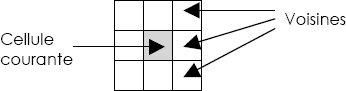
\epsfig {file=img/cellneighboor.png,width=6cm}}
	\caption{Une cellule et ses voisines}
	\label{fig:cellneighboor}
\end{figure}

D'autres variantes de ces r{\^e}gles sont d{\'e}finissables, dans la mesure o{\`u} chaque cellule conna{\^i}t l'{\'e}tat de ses huit voisines. Il suffit de faire varier le nombre de cellules vivantes n{\'e}cessaires pour en faire naitre une nouvelle, la maintenir en vie ou la faire mourir. Il faut pr{\'e}ciser que le jeu de la vie n'est pas vraiment un jeu au sens ludique, puisqu'il ne n{\'e}cessite aucun joueur ; il s'agit d'un automate cellulaire, un mod{\`e}le o{\`u} chaque {\'e}tat conduit m{\'e}caniquement {\`a} l'{\'e}tat suivant {\`a} partir de r{\`e}gles pr{\'e}-{\'e}tablies.~\\

Une {\'e}tude syst{\'e}matique de ce type de mod{\`e}le a {\'e}t{\'e} effectu{\'e}e par Stephen Wolfram au de 1980 {\`a} 2003~\cite{wolframNewKindScience}. 

% \clearpage

\subsection{Mod{\`e}le math{\'e}matique d'{\'e}cologie}
% Stephane Legendre (informaticien {\`a} la base), laboratoire ENS/CNRS sciences du vivant~\\
% Mod{\`e}le et simulation bact{\'e}rien (\textit{Pseudomonas fluorescens})~\\

\begin{minipage}{0.5\linewidth}
Des mod{\`e}les plus complexes ont {\'e}t{\'e} construits, toujours sur ce m{\^e}me principe d'un ensemble de r{\^e}gles math{\'e}matiques ou physiques simpleset d{\'e}finissant le d{\'e}roulement de la simulation et sa param{\`e}trisation~\cite{numericalEcology,spatialAutoCorrelation,speciesAssembl} : par exemple pour {\'e}tudier le gradient d'un produit ou pr{\'e}sence d'un autre organisme sur la survie d'organimses mod{\'e}lis{\'e}s. Chaque <<bact{\'e}rie>> ne peut avoir qu'un nombre limit{\'e} de <<concurrents>> (qualit{\'e} implicite d'un milieu renouvel{\'e}), gradient entre la surface et le fond de la <<boite de Petri>>...
\end{minipage}
\begin{minipage}{0.1\linewidth}\end{minipage}
\begin{minipage}{0.4\linewidth}
Un cycle de calcul dans ce type de mod{\'e}lisation peut se d{\'e}composer de la fa\c{c}on suivante :
\begin{enumerate}
	\item Reproduction
	\item Mutation
	\item Mouvement
	\item Comp{\'e}tition
	\item S{\'e}lection
\end{enumerate}
\end{minipage}~\\

\clearpage

\subsection{Les virus informatiques}

\begin{minipage}{0.6\linewidth}
%% Mutation des virus informatiques - exp{\'e}riences de vie artificielle
Mark A. Ludwig \textit{Mutation d'un virus}
\begin{itemize}
	\item Virus qui favorise l'{\'e}volution
	\item Mutations quasi ``al{\'e}atoires''
	\item Recherche du code des survivants
	\item M{\'e}canismes de reproduction
	\begin{itemize}	
		\item Modules inclus au virus
		\item Manipulation d'un {\'e}l{\'e}ment
	\end{itemize}
\end{itemize}
\end{minipage}
\begin{minipage}{0.1\linewidth}\end{minipage}
\begin{minipage}{0.3\linewidth}
Un m{\^e}me virus peut poss{\'e}der plusieurs fois le m{\^e}me moteur en copie interne : s{\'e}lection d'une partie du code et la copie est ajout{\'e}e {\`a} la fin.~\\
\end{minipage}~\\

\rule{10cm}{0.5mm}~\\

\begin{minipage}{0.6\linewidth}
Il y a dans ces exemples utilisation d'un moteur darwinien de s{\'e}lection g{\'e}n{\'e}tique : connaissant le risque de se faire prendre {\`a} chaque g{\'e}n{\'e}ration (utilisateur, antivirus), donc si le virus en r{\'e}chappe une fois, il faut pouvoir continuer, d'o{\`u} une conservation de son pass{\'e} <<g{\'e}n{\'e}tique>> et de son d{\'e}veloppement. Il y a donc ici une exploitation des informations g{\'e}n{\'e}tiques, associ{\'e} {\`a} un souvenir des mutations et la conservation des propri{\'e}t{\'e}s parentales.
\end{minipage}
\begin{minipage}{0.1\linewidth}\end{minipage}
\begin{minipage}{0.3\linewidth}
Diff{\'e}rents moteurs de fonctionnement
\begin{itemize}
	\item reproduction
	\item mutation
	\item analyse
	\item destruction
	\item contr{\^o}le
	\item m{\'e}moire {\'e}ventuelle
\end{itemize}
\end{minipage}~\\~\\

\subsection{Le jeu \textit{Creatures}}

La premi{\`e}re version grand public du jeu \textit{Creatures} est disponible en 1996 (pour Windows 95 et Mac OS Classic) ; l'objectif principal de ce mod{\`e}le de simulation est la mod{\'e}lisation de comportements adaptatifs en utilisation la vie artificielle~\cite{CliGra99,GraCli97,GraCli98,GrClMa96,GrClMa97}. Il ne s'agit plus vraiment ici d'automates cellulaires, les <<individus>> simul{\'e}s sont appel{\'e}s des \textbf{Norns} (\textit{Cyberlifogenis cutis}), et sont accompagn{\'e}s dans leur environnement virtuels par des Grendels (\textit{Cyberlifogenis vicious}) et des Ettins (\textit{Cyberlifogenis kleptomonicus}).~\\

% \clearpage

La simulation est fortement centr{\'e}e autour du syst{\`e}me nerveux des norns, les neurones sont organis{\'e}s en groupes (lobes, la terminologie biologique est reprise). Diff{\'e}rents param{\`e}tres d{\'e}finissent les changements d'{\'e}tats des neurones, ces param{\`e}tres sont identiques pour les neurones au sein d'un m{\^e}me lobe. Certains param{\`e}tres des neurones sont des r{\`e}gles de calcul de l'{\'e}tat (excitation, repos, relaxation...) ou de connection avec d'autres neurones au sein du m{\^e}me lobe ou vers d'autres lobes. Autour de ce mod{\`e}le de r{\'e}seau neuronal, une biochimie simple est simul{\'e}e et cod{\'e}e g{\'e}n{\'e}tiquement pour permettre une gestion des informations en fonction d'un syst{\`e}me hormonal (endocrinien) et d'un m{\'e}tabolisme basique.~\\

Lors de la cr{\'e}ation des commandes et fonctions associ{\'e}es aux g{\`e}nes il a {\'e}t{\'e} convenu de d{\'e}terminer les variables et les {\'e}carts de valeurs num{\'e}riques possibles. Pour certains types de g{\`e}nes cette valeur d{\'e}termine son (in)activit{\'e} (0 ou 1) et peut d{\'e}pendre de l'{\^a}ge de la vie du norn, d'autres sont fixes pour sa vie (apparence/immunit{\'e} sauf par accident ou de fa\c{c}on volontaire, comprises entre 1 et 26), et donne lieu qu'{\`a} l'expression d'un seul type de caract{\`e}re (ici une lettre qui d{\'e}termine l'identit{\'e} du norn).~\\

Enfin certains g{\`e}nes ont une variable dont le niveau d{\'e}termine l'activit{\'e} du g{\`e}ne (ex : g{\`e}nes des lobes du cerveau, le niveau de la variable d{\'e}termine dans quel domaine il exerce son activit{\'e} : sensoriel, conceptuel, d{\'e}cision, attention...) pour ce dernier type de g{\`e}ne la tol{\'e}rance pour la valeur de la variable est large et les ``cr{\'e}neaux'' o{\`u} l'activit{\'e} est d{\'e}termin{\'e}e sont larges pour {\'e}viter qu'une mutation ponctuelle ne modifie imm{\'e}diatement l'activit{\'e} du g{\`e}ne.~\\

Les mutations s'effectuent surtout lors de la reproduction (<<erreurs de transcriptions>>) et peuvent modifier les valeurs de diff{\'e}rentes fa\c{c}ons : changement de valeur (0/1), incr{\'e}mentation ou d{\'e}cr{\'e}mentation (apparence, immunit{\'e} et lobes), duplication/{\'e}limination du g{\`e}ne. La probabilit{\'e} de mutation est la m{\^e}me pour chaque g{\`e}ne (le processus recommence {\`a} chaque fois). En de rares {\'e}v{\`e}nements, des mutations peuvent se produire suite {\`a} une infection (agents pathog{\`e}nes ou autre) ou l'exposition {\`a} des <<radiations>>.~\\

\subsubsection{G{\'e}n{\'e}tique des norns}

Le g{\'e}nome des norn est haplo{\"i}de (un seul chromosome)~\cite{GraCli97}. Lors de la reproduction, les g{\`e}nes peuvent {\^e}tre dupliqu{\'e}s, mut{\'e}s voire d{\'e}l{\'e}t{\'e}s, avec certaines limitations pour certains g{\`e}nes et v{\'e}rifier la viabilit{\'e} (ou la non-viabilit{\'e}) d'un nouvel individu ; un crossing-over peut {\'e}galement {\^e}tre appliqu{\'e} entre les g{\`e}nes parentaux. Chaque g{\`e}ne poss{\`e}de un en-t{\^e}te pour indiquer s'il peut {\^e}tre mut{\'e}, dupliqu{\'e} ou d{\'e}l{\'e}t{\'e} (chaque crit{\`e}re n'est pas exclusif ou limitatif pour les autres), ainsi que l'activation du g{\`e}ne selon l'{\^a}ge.~\\

% \clearpage

Diff{\'e}rents types de g{\`e}nes sont d{\'e}finis dans \textit{Creatures}~\cite{GraCli97} : 
\begin{itemize}
	\item \textbf{Chemicals // InitialConcentration} ou {\'e}l{\'e}ments chimiques : ce sont des variables d{\'e}finies g{\'e}n{\'e}tiquement indiquant des concentrations de produits dans l'organisme du norn, sans aucune d{\'e}finition pr{\'e}cise des propri{\'e}t{\'e}s des produits. \emph{Chaque g{\`e}ne de ce type indique les num{\'e}ros des produits, leur nom, leur concentration, leur dur{\'e}e de demi-vie... }
	\item \textbf{Emitters} : ces {\'e}l{\'e}ments sont produits par des objets {\'e}metteurs (d{\'e}finis g{\'e}n{\'e}tiquement) et peuvent {\^e}tre reli{\'e}s {\`a} des sorties du r{\'e}seau de neurones. Le changement de valeur de l'{\'e}l{\'e}ment reli{\'e} provoque un changem{\`u}ent de sortie de l'{\'e}metteur. \emph{Les g{\`e}nes de ce type contiennent le ``lieu'' d'{\'e}mission, le num{\'e}ro du produit et le fonctionnement de l'{\'e}metteur. }
	\item \textbf{Receptors} : ces {\'e}l{\'e}ments ont le fonctionnement oppos{\'e} des r{\'e}cepteurs, ce sont des entr{\'e}es du syst{\`e}me nerveux. \emph{Les g{\`e}nes des recepteurs contiennent le num{\'e}ro du produit auquel r{\'e}agir, le niveau {\`a} partir duquel r{\'e}gir et le signal d'entr{\'e}e. }
	\item \textbf{Reactions}~\label{creatures:reactions} : les r{\'e}actions chimiques sont le centre du m{\'e}tabolisme des norns, et peuvent avoir une large palette de comportements :  
	\begin{itemize}
		\item $A + B \rightarrow C + D$ : r{\'e}action chimique standard
		\item $A + B \rightarrow C$ : fusion de r{\'e}actifs
		\item $A \rightarrow \emptyset$ : diminution (l'inverse n'est pas permis)
		\item $A + B \rightarrow A + C$ : catalyse (A est inchang{\'e})
		\item $A + B \rightarrow A$ : diminution catalytique de B
	\end{itemize}
	\emph{Les g{\`e}nes d{\'e}finissant les r{\'e}actions chimiques d{\'e}finissent les c\oe fficients et la vitesse de r{\'e}action. }
	\item \textbf{G{\`e}nes d'apparence et du syst{\`e}me nerveux} (incluant les Stimulus et les Instincts, qui ne seront pas d{\'e}taill{\'e}s ici, mais pour lesquels de nombreuses ressources sont disponibles~\cite{CliGra99,GraCli97,GraCli98,GrClMa96,GrClMa97}.
	\item De plus, des infections bact{\'e}riennes des norns sont possibles, ils disposent d'un syst{\`e}me immunitaire qui r{\'e}agit aux antig{\`e}nes bact{\'e}riens par une production d'anticorps.
\end{itemize}

\subsubsection{Outils autour de \textit{Creatures <<1.0>>}}

Les logiciels inclus {\`a} la simulation peuvent lire et modifier les diff{\'e}rents fichiers de cette mod{\'e}lisation, les afficher et les interpr{\'e}ter pour l'utilisateur. Les fonctionnalit{\'e}s sont les suivantes :
\begin{itemize}
	\item \textbf{CGM (Creatures GenMan) // Genetic Kit} : Analyse du g{\'e}nome d'un norn (g{\`e}ne par g{\`e}ne, affichage de ce {\`a} quoi correspond la variable de chaque g{\`e}ne), croisement entre deux g{\'e}nomes, introduction d'un nouveau norn avec un g{\'e}nome s{\'e}lectionn{\'e} et d'autres param{\`e}tres (stade de la vie, sexe...), 
	\item \textbf{Object injector} : fait introduire des objets, permet la programmation de nouveaux objets (programmation simplifi{\'e}e selon cat{\'e}gorie d'objets), 
	\item \textbf{BORG} : Interaction directe avec le m{\'e}tabolisme interne des norns, s{\'e}lection des objets et organismes non s{\'e}lectionnables autrement au sein de la simulation (plantes, objets d'interactions comme des jouets...). 
\end{itemize}~\\

Chaque objet, pr{\'e}sent dans l'environnement, est caract{\'e}ris{\'e} par :
\begin{itemize}
	\item Des variables (vitales, {\`a} ajouter, {\`a} soustraire selon le programme) suivant une liste normalis{\'e}e. 
	\item Une information g{\'e}n{\'e}tique (ou programme sp{\'e}cifique de l'objet) (le code g{\'e}n{\'e}tique peut {\^e}tre pr{\'e}vu de fa\c{c}on {\`a} autoriser la vie, mais aussi des op{\'e}rations <<simples>> : augmenter une variable, diminuer une variable, faire un d{\'e}placement...). % (necessit{\'e} d'un code tr{\`e}s large, {\'e}tape par {\'e}tape pour certains {\'e}l{\'e}ments comme virus et reproduction : recherche objet {\`a} contaminer ou partenaire de reprodution, copie du code ou croisement des codes...). 
\end{itemize}~\\

\subsubsection{{\'E}volution du jeu : \textit{Creatures}, 2, 3, \textit{Docking Station}}

Des versions ult{\'e}rieures de ce jeu ont permit de faire {\'e}voluer diff{\'e}rents aspects du jeu et du mod{\`e}le sous-jacent. Les {\'e}l{\'e}ments qui ont {\'e}volu{\'e}s sont les graphismes, un syst{\`e}me de feddback (lobe de r{\'e}gulation) dans la version 2, l'annotation du g{\'e}nome et son formalisme avanc{\'e} dans la version 3, avec l'apparition des organes au sein des norns et la liaison des g{\`e}nes avec ces organes. De plus, les r{\^e}gles de calcul du r{\'e}seau de neurones ont {\'e}volu{\'e}es (les \emph{State Variable Rules}) de fa\c{c}on a permettre la construction de r{\^e}gles plus {\'e}labor{\'e}es.~\\

Quelques notes de recherches exp{\'e}rimentales sur le fonctionnement et la documentation de  \textit{Creatures} sont pr{\'e}sent{\'e}es dans ce m{\'e}moire dans leur version originale (en anglais), Ces notes concernent la premi{\`e}re et la seconde version du logiciel et proviennent notamment du \emph{Creatures Developper Ressources}~\cite{CreaturesDeveloperRessources} et du site \emph{geNornIcs}~\cite{genornics}, disponibles respectivement aux adresses suivantes : 
\begin{itemize}
	\item $<$\textit{http://www.double.co.nz/creatures/}$>$~\cite{CreaturesDeveloperRessources}
	\item $<$\textit{http://meliweb.net/creatures/}$>$~\cite{genornics}
\end{itemize}~\\

L'int{\'e}r{\^e}t de cette section est de fournir une documentation existente sur une cr{\'e}ation r{\'e}elle et de finaliser un {\'e}tat de l'art sur ce type de d{\'e}veloppement, au d{\'e}part purement accad{\'e}mique puis commercial dans le cas de \emph{Creatures} ; un tel d{\'e}veloppement pouvant {\^e}tre repris pour mod{\'e}liser un ensemble biologique complexe (organismes dans leur milieu, g{\`e}nes, {\'e}volution...) et permettre {\`a} une communaut{\'e} d'utilisateurs d'{\'e}tudier un tel mod{\`e}le et d'y ajouter diverses cr{\'e}ations, de d{\'e}couvrir diverses mutations voire une {\'e}volution.~\\

\clearpage

\section{Special notes about Genetics of Creatures}

\subsection{Genetics} % CDR -- 

The behavior of a norn and its interaction with the environment within Creatures is controlled by its Digital DNA. This DNA code can be modified using the Creatures Genetics Kit. The Genetics Kit is the official means of editing a norns genome but there are various third party tools available as well. See the links page for other sites that may contain such utilities.~\\

While this documentation concentrates mainly on the Norn brain lobes there are a number of other genes that are modifiable via the Genetics Kit. The online help in the Genetics Kit is not very helpful when it comes to descriptions of the individual fields within each gene dialog box. Follow the links below to get information on the various fields for each gene dialog in the Genetics Kit based upon information I've gathered on the net and experiments I've performed.~\\

% 	\begin{center}
%		\begin{tabular}{p{0.6\textwidth} p{0.4\textwidth} }
\begin{minipage}{0.5\linewidth}
			\subsubsection{Genes}
			\begin{itemize}
				\item Brain Lobe
				\item Chemical Receptor
				\item Chemical Emitter
				\item Chemical Reaction
				\item Chemical Half-Lives
				\item Chemical Initial Concentrations
				\item Stimulus
				\item Genus
				\item Appearance
				\item Pose
				\item Gait
				\item Instinct
				\item Pigment
				\item Pigment Bleed
			\end{itemize}
\end{minipage}
			% &
\begin{minipage}{0.1\linewidth}\end{minipage}
\begin{minipage}{0.4\linewidth}
			\subsubsection{Reference Tables}
			\begin{itemize}
				\item State Variable Rules
				\item Cell List connection~\cite{genornics}
				\item Brain Map and Models~\cite{genornics}
			\end{itemize}
			
			\rule{3cm}{0.25mm}
			
			\rule{3cm}{0.25mm}
			
			\emph{The information presented here was written for Creatures 1 but all the information is still valid for Creatures 2 genetics. I have not yet updated the screenshots of the genetics kit for Creatures 2 but not much new was added that needs explanation.}
\end{minipage}
%			\\
%		\end{tabular}
%	\end{center}
~\\~\\
\rule{10cm}{0.5mm}

% \clearpage

\subsection{Brain Lobes} % CDR -- 

The brain lobe is one of the most complicated portions of norn genetics. The Cyberlife Genetics Kit provides the ability to add, delete or modify brain lobes. The dialog box for modifying brain lobes contains a bewildering number of options. The purpose of this brain lobe discussion is to describe what each of these options does.~\footnotesize{Note 08/10/1999: The information on brain lobes below was created for Creatures 1. All the information is still valid for Creatures 2 genomes, but the screen shots show the Creatures 1 genetics kit.}~\normalsize{}~\\

% \clearpage

The descriptions of the brain lobe settings shown here have mostly been discovered through experimentation. The tutorials available in another section  describes how most of the information was found. The purpose of this section is to provide a single place where all the information gathered through the tutorials and other places can be placed for easy use. It will be updated frequently as I discover new things.

\subsubsection{Overview}

Most standard norns have nine brains lobes. A number of the lobes are 'special' in that they have a particular function hard-coded within the Creatures executable. A limited amount of genetic modification can be done to these lobes as most of their functionality is provided through the Creatures system. The other lobes are completely genetically defined and this is where some of the most interesting modifications to a Norn can be made.~\\

\clearpage

A brain lobe sits within a 64x48 grid of neurones (often referred to here as cells). A lobe has a location within this brain grid described as an (X, Y) coordinate and (width, height). Each lobe therefore has a set size measured in neurones. Each neurone in a lobe has a numeric value associated with it known as the 'state' represented as a number from between 0 and 255 inclusive. The current value of the 'state' of a neuron indicates the level of activity. The value of the neurone 'state' can be set via the Creatures executable directly, CAOS macro code, or via dendritic links from other cells in other brain lobes. In this manner a network of cells and lobes is created that ultimately forms the 'brain' or neural net of the norn.~\\

All neurones within a single lobe behave in a similar manner to perform some function. Each lobe has genetically defined information associated with it that affects the neurones in that lobe. So a brain lobe is really a group of neurones that perform in a similar manner.~\\

%\rule{10cm}{0.5mm}~\\~\\
A detailed description of the genetically defined information associated with each lobe follows. This is the information that was obtained through experimentation. After this a brief description of the functionality of the brain lobes in a standard norn is provided. This document will conclude with some ideas and thoughts on future brain modifications that could be made to improve or modify a norns behavior.

\subsubsection{Brain Lobe Genetics - Genes' Header}

The Cyberlife Genetics Kit has a 'tabbed' dialog box for modifying the genetic information associated with a brain lobe. Each page of the dialog box holds information about the lobe and the breakdown below will be done page by page as defined by the genetics kit.~\\~\\~\\

\textbf{\textit{General Page}}~\\

\begin{minipage}{0.4\linewidth}
\begin{figure}[H]
	\centerline {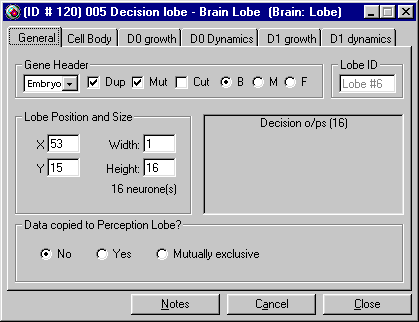
\epsfig {file=img/brain_general.png,width=5cm}} % 14.8cm
	\caption{General Interface for Brain Genetics Design}
	\label{fig:brain_general}
\end{figure}
\end{minipage}
\begin{minipage}{0.1\linewidth}\end{minipage}
\begin{minipage}{0.5\linewidth}
The example dialog given here is from the Decision lobe of a Ron norn. The 'general' page provides the standard gene header information that describes when the gene switches on, how mutations affect it and the required sex of the norn for the gene to switch on. Also included is information on the placement of the lobe within the brain grid, a description of the lobe, a unique numeric identifier for the lobe and an indication as to whether lobe data is copied to the perception lobe.
\end{minipage}~\\

\textbf{\textit{Gene Header}}
\begin{itemize}
	\item[] \emph{Embryo} : This field indicates the age at which the brain lobe gene will switch on. Most brain lobes turn on at the 'Embryo' stage to ensure they operate correctly as soon as the norn is born. I know of no lobes that are turned on at different ages and I don't know if this functionality even works. This has been added to the list of issues to explore.
	\item[] \emph{Dup} : If this flag is checked then the lobe can be duplicated as a genetic mutation. That is, multiple copies of this lobe will be able to exist due to mutation.
	\item[] \emph{Mut} : Sets whether genetic mutations can be applied to the values contained within this brain lobe.
	\item[] \emph{Cut} : If set the brain lobe can be removed during breeding or as the result of mutation. Most brain lobes have this unchecked as a norn without any of the standard lobes would not be able to function.
	\item[] \emph{B/M/F} : Defines the gender that this brain lobe will switch on. This could potentially be used to create norns that have different intelligence levels or behaviour depending on the gender of the norn. I haven't tested if this functionality actually works. This has been added to the list of issues to explore.
\end{itemize}~\\

\clearpage

\textbf{\textit{Lobe Id}}
\begin{itemize}
	\item[] \emph{Lobe \#} : Contains the numeric identifier for the brain lobe. This is assigned automatically by the genetics kit and cannot be changed. The first 8 numbers (0 through to 7) correspond to specific lobes that are hard-coded within the Creatures executable. If you number a lobe with one of these hard coded numbers (using a hex editor or such like) then Creatures may stomp over your neurone values at any time so be warned.
\end{itemize}

% \clearpage
\textbf{\textit{Lobe Position and Size}}
\begin{itemize}
	\item[] \emph{X} : Contains the X coordinate of the lobes location within the brain grid. I don't know what the effect of overlapping brain lobes will be. Added to the issues list.
	\item[] \emph{Y} : Contains the Y coordinate of the lobes location within the brain grid.
	\item[] \emph{Width} : Contains the amount of neurones in the X direction that the lobe uses within the brain grid.
	\item[] \emph{Height} : Contains the amount of neurones in the Y direction that the lobe uses within the brain grid.
\end{itemize}

The total number of neurones contained within the lobe is calculated as (Width * Height).~\\ % and displayed in the dialog box.~\\ % I do not know if the layout of the lobe or location within the brain grid has any affect on the functionality of the lobe. % Added to the issues list.

\textbf{\textit{Description}}

This contains a description of the functionality of the brain lobe and is not editable. I think only the standard brain lobes have descriptions associated with them. All additional lobes get a default like 'Interneurone lobe'.~\\

\textbf{\textit{Data Copied to Perception Lobe}}
\begin{itemize}
	\item[] \emph{No} : None of the information in this brain lobe will be duplicated in the perception lobe (lobe 0).
	\item[] \emph{Yes} : Every neurone within this brain lobe will have its state value duplicated in the perception lobe. See the perception tutorial for details.
\item[] \textit{Mutually Exclusive} : A lobe marked as mutually exclusive affects the way dendrites are formed between the perception lobe and the concept lobe. If a lobe is marked as mutually exclusive then only one cell from this lobe may contribute to the forming of a particular concept in the concept lobe. See the perception tutorial for details. 
\end{itemize}

\subsubsection{Cell Body Page}

\begin{minipage}{0.5\linewidth}
\begin{figure}[H]
	\centerline {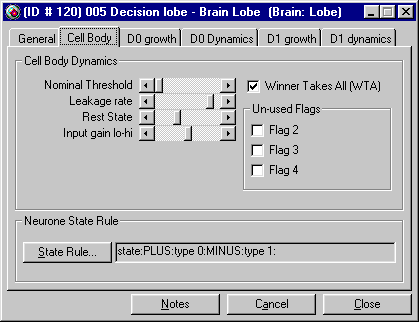
\epsfig {file=img/brain_cellbody.png,width=5cm}} % 14.8cm
	\caption{Cell Body Interface for Brain Genetics Design}
	\label{fig:brain_cellbody}
\end{figure}
\end{minipage}
\begin{minipage}{0.1\linewidth}\end{minipage}
\begin{minipage}{0.4\linewidth}
The 'Cell Body' page provides information associated with each neurone (otherwise known as 'cell') within the brain lobe. It is here that the behaviour of the neurones are defined. Much of the information obtained about this page is from tutorial one and tutorial two.
\end{minipage}~\\

% \clearpage

\textbf{\textit{Cell Body Dynamics}}
\begin{itemize}
	\item[] \emph{Nominal Threshold} : This is a number with a value from 0 through to 255. When the state is set for a neurone it will not fire unless the value of the neurone state is greater than this threshold. The value of the neurone after firing will be state minus threshold.
	\item[] \emph{Leakage Rate} : This defines the speed at which the state will drop from its current value to its rest state. It has values like 'Instantly', '5 Seconds', right through to '52 Years' and is represented by a number from 0 to 255.
	\item[] \emph{Rest State} : This is the resting state of the neurone. That is, if the neurone has not been fired or activated it will sit on the value set here. The value is from 0 through to 255.
	% \item[] \emph{Input gain lo-hi} : I have no idea what this value does. Added to issues list.
	\item[] \emph{Winner Takes All} : If this flag is checked then the lobe is a winner-takes-all lobe. This means that after all the neurone values for the lobe are calculated the highest firing neurone (highest state value) is the only one that fires and all the other neurones have their output value set to zero. An example is the decision lobe where only one decision can be made.
\end{itemize}
\clearpage
% \textbf{\textit{Un-used Flags}} : These flags do not appear to be used in any way.~\\

\textbf{\textit{Neurone State Rule}}

An SVRule is like a miniature program written in a special programming language, which has a number of 'opcodes' or operations that it can perform on various pieces of data. Only eight individual opcodes are allowed in an SVRule making it very small and fast to execute - the SVRule for every cell in the brain must execute 10 times per second! -- \emph{\underline{State Rule}} : The SVRule defined here is used to calculate the new state value of a neurone. The result of the SVRule becomes the state value of the neurone. In this way the state for neurones within lobes can be defined genetically and different calculations can be performed depending upon the task of the lobe. The SVRule possibilities are huge and can be of a great complexity. Remember that SVRules are used in a number of places in a brain lobe but the specific one here is only used to calculate the value of each neurone 'state'. % See the state variable rule page for a description of SVRules in general and what each opcode does.

\subsubsection{D0 Growth Page}

\begin{minipage}{0.6\linewidth}
\begin{figure}[H]
	\centerline {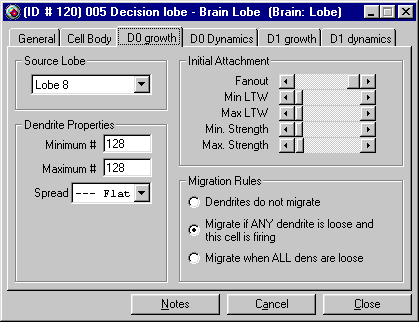
\epsfig {file=img/brain_d0growth.png,width=5cm}} % 14.8cm
	\caption{D0 growth Interface for Brain Genetics Design}
	\label{fig:brain_d0growth}
\end{figure}
\end{minipage}
\begin{minipage}{0.1\linewidth}\end{minipage}
\begin{minipage}{0.4\linewidth}
This is one of the first pages that describes the behaviour of dendrite connections in a lobe. Dendrites are to the brain lobes as wiring is to integrated circuits. They connect the neurones in different lobes and allow information to travel between them. Each brain lobe can have dendrite connections with up to two different source lobes. These are described as 'type0' dendrites and 'type1' dendrites. This page describes the settings for 'type0' dendrites.
\end{minipage}~\\~\\

% Dendrite connections are probably the most complicated part of the norn brain structure and much of what is described here is still being explored by me. If you don't understand any of what follows please email me and I'll make an effort to make it easier to understand.\\

\textbf{\textit{Source Lobe}} : This defines the brain lobe these dendrites are connected to. Data flows from neurones in the source lobe defined here to neurones in this brain lobe. ~\\ % \underline{Brain lobe construction where information comes from.}~\\ % does not define where information goes to but

\textbf{\textit{Dendrite Properties}}
\begin{itemize}
	\item[] \emph{Minimum \#} : Defines the minimum number of dendrites that will be connected between each cell in the current lobe and a source lobe cell.
	\item[] \emph{Maximum \#} : Defines the maximum number of dendrites that will be connected between each cell in the current lobe and a cell in the source. %lobe. 
	\item At birth a norn will have a random brain wiring pattern set up. Each cell will have a number of dendrites ranging between the minimum and maximum number defined here. As dendrites migrate the minimum and maximum numbers are important as they define whether there is room for a new dendrite connection to be made or removed. The decision on how many dendrites to use when creating a lobe depends upon the type of information to obtain from the source lobe and what to do with it.
	\item[] \emph{Spread} : This appears to define the pattern used to define the 'fanning' of the dendrite connection between the current lobe and the source lobe. The options are 'Flat', 'Normal', 'Saw' and 'waS'. If the spread is 'flat' then there will be two dendrites connecting neurone x from the source lobe to neurone x in the destination lobe, then (x+1) to (x+1), etc. With the other settings, a connection from neurone x in the current lobe to neurones x and (x+1) in the source lobe, from neurone (x+1) to neurones (x+1) and (x+2), etc. The exact layout of the dendrites will also depend on the 'fanout' value described later.
\end{itemize}~\\

\textbf{\textit{Initial Attachment}}
\begin{itemize}
	\item[] \emph{Fanout} : When the dendrite wiring for a brain lobe is initially created on birth of a creature, this value defines how each dendrite connection from the current lobe 'fans out' to neurones in the source lobe. The value varies from 0 through to 8.
	\item[] \emph{Min LTW} : A number ranging from 0 through to 255 described as the minimum Long Term Weight. A dendrite has a value known as the long term weight (LTW) and it has a minimum and maximum possible value. It's actual value floats somewhere in between the minimum and maximum. % The function of LTW is described in the dendrite section. These numbers are only used when initially setting the values of the dendrite upon birth. % of a norn.
	\item[] \emph{Max LTW} : The maximum value of the Long Term Weight as a number from 0 through to 255. It must be equal to or greater than the min LTW.~\\
	\item[] \emph{Min Strength} : Each dendrite has a strength value represented as a number from 0 through to 255. The strength represents how 'strong' the link between the source neurone and the current neurone. When the strength is '0' then the dendrite may migrate as the link is not strong. The minimum number defined here is used for the initial wiring of the brain lobe and for initial values after dendrite migration.
	\item[] \emph{Max Strength} : The maximum strength value that can be assigned to a dendrite on initial brain wiring.
\end{itemize}~\\

\textbf{\textit{Migration Rules}}

The radio button settings here define how dendrites will migrate between cells. An example of dendritic migration is the connections between the perception lobe and the concept lobe. The perception lobe is the source lobe and the concept lobe is the destination lobe. There may be several neurones from the source lobe connected to a single cell in the destination lobe. As a norn is punished then the connections on the source lobe neurones will migrate to other source lobe neurones to form more appropriate 'concepts' for the norn to learn and make decisions from. 
\begin{itemize}
	\item[] \emph{Dendrites do not migrate} : With this setting dendrites will not migrate at all and stay with the initial connections made at birth. This is most often used when the maximum and minimum number of dendrites is one with a flat spread. Nothing needs to migrate.
	\item[] \emph{Migrate if ANY dendrite is loose and this cell is firing} : If a neurone in the current lobe has a number of dendrites attached to a source lobe, this setting will cause the dendrites to migrate if any of these dendrites has a strength of zero and the neurone is currently firing. If a dendrite in the neurone is loose (ie. has strength of zero) but the neurone is not firing then no migration will occur. Only one of the dendrites has to be loose for the migration to occur.
	\item[] \emph{Migrate when ALL dendrites are loose} : In this case every dendrite from a given neurone in the current lobe must have a strength of zero for the dendrites to migrate. If only one is zero then no migration will occur.
\end{itemize}

% \clearpage

\subsubsection{D0 Dynamics Page}

\begin{minipage}{0.4\linewidth}
\begin{figure}[H]
	\centerline {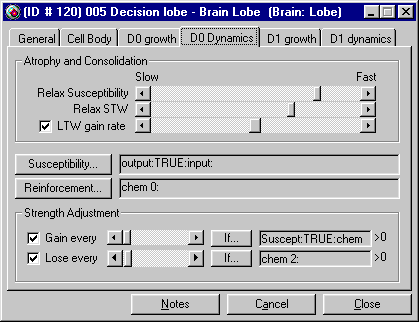
\epsfig {file=img/brain_d0dynamics.png,width=5cm}} % 14.8cm
	\caption{D0 dynamics Interface for Brain Genetics Design}
	\label{fig:brain_d0dynamics}
\end{figure}
\end{minipage}
\begin{minipage}{0.1\linewidth}\end{minipage}
\begin{minipage}{0.5\linewidth}
This is probably the most complicated portion of norn genetics. The definition of the dynamics of the dendrites. The 'D0' page describes the dynamics for the 'type0' dendrites. The dynamics defines how the strength value of a dendrite is adjusted, how the STW and LTW are adjusted, etc.~\\

A number of values are associated with a dendrite. A brief description follows to make it easier to understand what the settings on this page mean. Most of these definitions were obtained from the paper by Steve Grand \textit{et al} obtained from the Cyberlife web site.
\end{minipage}~\\

\begin{itemize}
	\item[] \emph{STW} : Short Term Weight - used to modulate input signals. STW is constantly relaxing towards LTW. It is the STW combined with the input value from the source lobe that is used to calculate the 'dendrite value'. The formula used appears to be: $dendrite value = source cell * ( stw / 255 )$~\\
where 'source cell' is the value of the cell that this dendrite is attached to from the source lobe and 'stw' is the dendrites current short term weight value. \underline{The formula for calculation of STW appears to be: } $stw = ltw + ( susceptibility / 255 ) * reinforcement$. 
	\item[] \emph{LTW} : Long Term Weight - acts as a rest state for STW and provides statistical response to reinforcement. LTW is constantly rising towards STW. LTW and STW move towards each other at different rates (and these rates are defined genetically).
	\item[] \emph{Susceptibility}: Current susceptibility to reinforcement. As can be seen in the STW calculation above, the susceptibility modulates the reinforcement value. So the higher the 'susceptibility' value, the more 'reinforcement' affects the short term weight value. 
	\item[] \emph{Strength} : Controls dendrite migration. Represents how 'strong' the dendrite link is. If strength hits zero then the link is not strong and may migrate.
\end{itemize}
\clearpage

\textbf{\textit{Atrophy and Consolidation}}
\begin{itemize}
	\item[] \emph{Relax Susceptibility} : The is the half-life of the 'susceptibility' of the dendrite. It is a value from 0 through to 255 and defines a time interval in a similar manner to that of 'Leakage Rate' in 'Cell Body Dynamics'. The value shown in the image above is 20 seconds. So when the susceptibility of a dendrite is set via the Susceptibility SVRule this setting describes how quickly it 'relaxes' back to the rest state. The relationship between this value and the susceptibility SVRule is similar to that of 'Leakage Rate' and 'State SVRule' in the 'Cell Body' page.
	\item[] \emph{Relax STW} : This is the half-life or relaxation rate of the Short Term Weight value for the dendrite. The value in the image above represents 5 minutes. Once again it is a number from 0 through to 255 representing a time span. The STW relaxes towards the Long Term Weight (LTW) value of the dendrite. This relax rate sets the speed of that relaxation.
	\item[] \emph{LTW Gain Rate} : If this option is checked then LTW constantly rises towards STW at the rate defined in the slider box. This number is a rate in the same manner as all the other leakage rates (even through the genetics kit does not display it as such). For example, if set to 10 seconds (a value of 40) then the LTW will increment by one every 10 seconds until it reaches its rest state (which is the value of STW).
	\item[] \emph{Susceptibility} : An SVRule that defines how the susceptibility to reinforcement for that dendrite. The higher the value of the result of this svrule, the more effect 'reinforcement' has on the value of STW. The SVRule defined in the image above basically says if there is an output value for the cell (ie. it is firing) then the susceptibility of the dendrite is equal to that of the input value. 
	\item[] \emph{Reinforcement} : This is the SVRule used to compute changes in STW. Typically it is set to the value of some chemical. This chemical is adjusted using the various receptors/emitters available in a norn. The STW is increased based upon the value computed by this SVRule modulated by the value of the susceptibility SVrule. In the example above it means that STW is adjusted when the amount of brain lobe chemical 0 changes in this norn.
\end{itemize}

The relationship between STW, LTW, susceptibility and reinforcement is shown by the following formulae that is used to calculate the values: 
$dendrite value = source cell * ( stw / 255 )$ and $stw = ltw + ( susceptibility / 255 ) * reinforcement$.~\\

\textbf{\textit{Strength Adjustment}}
\begin{itemize}
	\item[] \emph{Gain Every} : If this is checked then the strength value of the dendrite connection will be increased by the value indicated in the slider (from 0 through to 255) if the result of the given SVRule expression is greater than zero. The SVRule given above is 'Suscept:TRUE:chem0:TRUE:STW'. I believe that this expression means that if the susceptibility of the connection is greater than zero and chemical 0 is greater than zero then the value of the expression is STW. So the dendrite will be strengthened if it is susceptible to reinforcement, has chemical 0 and the STW is greater than zero.
	\item[] \emph{Lose Every} : If this is checked then the strength value of the dendrite connection will be decreased by the value indicated in the slider (from 0 through to 255) if the result of the given SVRule expression is greater than zero. The SVRule given above is 'chem 2'. So if the value of chemical 2 is greater than zero then the strength of the dendrite will be reduced.
\end{itemize}

\subsubsection{Dendrite Overview}

This is a brief outline of how dendrite values are calculated mostly obtained from the technical papers available at the cyberlife web site. I'll add to this and hopefully provide some programs that demonstrate how things work to make it easier to understand. The following is quoted from one of the technical papers by Steve Grand \textit{et al}:~\\

% \clearpage

\emph{After disturbance, both the STW and the LTW relax exponentially towards other, with the LTW being the slower. The STW therefore reacts strongly to individual reinforcement episodes, while the LTW effectively computes a moving average of many STW disturbances: if a creature meets with situation X and finds that its chosen course of action was undesirable, then it should immediately be strongly disinclined to repeat the action, especially as many of the incentives to do so may still be present. However, situation X may not always be as bad as first experience suggests, and so the creatures long-term interpretation should be less sweeping}~\\

\clearpage

\emph{Dendritic Migration. The initial wiring is defined at birth according to a small number of genetic rules. Generally, neurones attempt to connect from one lobe to another in a direct spatial mapping, with multiple dendrites fanning out in a specified distribution to either side of the optimum source cell. After birth, however, individual dendrites may migrate and form new connections (always within the same source lobe). Periodically, a Strength value change is computed for each synapse using SVRules, often in response to chemical changes. If the Strength falls to zero, the dendrite disconnects and follows the appropriate rule about how to find a new connection. These migration rules were chosen in order to fulfill the requirements for the initial brain model.}

% \rule{10cm}{0.5mm}~\\

\subsection{Chemical Emitter} % CDR -- 

\subsubsection{Overview}

A chemical emitter gene controls the injection of a particular chemical into the norn based upon data retrieved from some Organ, Tissue or Locus within the norn. The Organ, Tissue or Locus is a data value controlled by the Creatures executable ranging in value from 0 through to 255. It can represent a brain cell, external stimuli or other things selected from the dialog box. Every given time period the Organ, Tissue or Locus is examined and compared against a number of settings defined in this gene. Depending upon the results of this comparison an amount of chemical can be injected into the norn.~\\

% \clearpage

\begin{minipage}{0.5\linewidth}
\subsubsection{Dialog Box}
\begin{figure}[H]
	\centerline {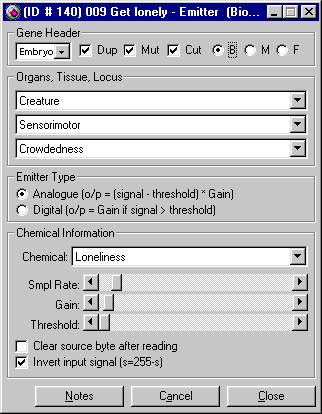
\epsfig {file=img/chemical_emitter.png,width=5.20cm}} % 11.35cm
	\caption{Interface for Chemical Emitter Design}
	\label{fig:chemical_emitter}
\end{figure}
\subsubsection{Breakdown -- \emph{Gene Header}}
\end{minipage}
\begin{minipage}{0.1\linewidth}\end{minipage}
\begin{minipage}{0.45\linewidth}
% \clearpage
\textbf{\textit{Gene Header}}~\\
\begin{itemize}
	\item[] \emph{Embryo} : This field indicates the age at which this gene will switch on. Most genes turn on at the 'Embryo' stage to ensure they operate correctly as soon as the norn is born. 
	\item[] \emph{Dup} : If this flag is checked then the gene can be duplicated as a genetic mutation. That is, multiple copies of this gene will be able to exist due to mutation.
	\item[] \emph{Mut} : Sets whether genetic mutations can be applied to the values contained within this gene.
	\item[] \emph{Cut} : If set the gene can be removed during breeding or as the result of mutation. 
	\item[] \emph{B/M/F} : Defines the gender that this gene will switch on. This is often used to select between genes that involve male or female functionality (eg. hormones).
\end{itemize}
\end{minipage}~\\~\\

% \textbf{\textit{Organs, Tissue, Locus}}~\\

% Defines the area of the norn that will be examined to calculate how much (if any) chemical to inject into the norn. Each of the options is represented by a data value ranging from 0 through to 255. The following table describes each possible option.~\\

%% %% http://www.ukonline.be/programmation/latex/tutoriel/chapitre13/page4.php %% table, rotate, longtable
%		\begin{longtable}{|p{0.15\textwidth}|p{0.20\textwidth}|p{0.65\textwidth}|}
%		\hline \rowcolor[gray]{0.50} \multicolumn{3}{|c|}{Organs, tissues, locus informations and description for Emitters} \\
%		\hline \rowcolor[gray]{0.75} \textbf{Box 1} & \textbf{Box 2} & \textbf{Box 3} \\ \hline
%		\endfirsthead
%		\hline \rowcolor[gray]{0.50} \multicolumn{3}{|c|}{Organs, tissues, locus informations and description for Emitters} \\
%		\hline \rowcolor[gray]{0.75} \textbf{Box 1} & \textbf{Box 2} & \textbf{Box 3} \\ \hline
%		\endhead
%		\hline 
%		\endfoot
%
%		Brain & Any Brain Lobe & \textbf{Lobe Activity} \\
%		\cline{3-3} % \hline
%				&	& \emph{Still to be investigated.} \\
%		\cline{3-3} % \hline
%				&	& \textbf{\# Loose Dens/Cells type 0} \\
%		\cline{3-3} % \hline
%				&	& \emph{Still to be investigated.} \\
%		\cline{3-3} % \hline
%				&	& \textbf{\# Loose Dens/Cells type 1} \\
%		\cline{3-3} % \hline
%				&	& \emph{Still to be investigated.} \\
%		\cline{3-3} % \hline
%				&	& \textbf{Cell(n) Output} \\
%		\cline{3-3} % \hline
%				&	& Represents the output value of the given cell in the brain lobe. See the brain lobe page for details on brain cells. \\
%		\hline \hline
%			Creature	&	Somatic	&	\textbf{Muscle Energy Used} \\
%		\cline{3-3} % \hline
%				&	& \emph{Still to be investigated.} \\
%		\cline{2-3} % \hline
%				&	Circulatory	& \textbf{Floating recip-emit n} \\
%		\cline{3-3} % \hline
%				&	& A floating recip--emit is a place that a receptor can use for storing a data value from 0--255 which an emitter can then use for any purpose. It's a means of linking a receptor directly to an emitter without going through a brain lobe. There are up to eight of these numbered from 0--7 (the 'n'). The life kit norns use this for the hunger/glycogen equation. \\
%		\cline{2-3} % \hline
%				&	Reproductive	& \textbf{I am fertile (egg/sperm ready)} \\
%		\cline{3-3} % \hline
%				&	& This will be a value of 0 until the norn becomes fertile in which case it will be 255. \emph{(Not confirmed, to be investigated).} \\
%		\cline{3-3} % \hline
%				&	& \textbf{I am pregnant (egg\&sperm ready)} \\
%		\cline{3-3} % \hline
%				&	& This will be a value of 0 until the norn becomes pregnant in which case it will be 255. \emph{(Not confirmed, to be investigated).} \\
%		\cline{2-3} % \hline
%				&	Immune	& \textbf{I'm dead (post mortem chemistry)} \\
%		\cline{3-3} % \hline
%				&	& This will be a value of 0 while the norn is alive. When the norn dies it will be 255. \emph{(Not confirmed, to be investigated).} \\
%		\cline{2-3} % \hline
%				&	Sensorimotor	& \textbf{Permanently Active (255)} \\
%		\cline{3-3} % \hline
%				&	& Always produces a value of 255. \emph{(Not confirmed, to be investigated).} \\
%		\cline{3-3} % \hline
%				&	& \textbf{I'm Asleep (255)} \\
%		\cline{3-3} % \hline
%				&	& This will be a value of 0 while the norn is awake. When the norn sleeps it will be 255. \emph{(Not confirmed, to be investigated).} \\
%		\cline{3-3} % \hline
%				&	& \textbf{Air is this cold} \\
%		\cline{3-3} % \hline
%				&	& This is always zero. It is not connected in Creatures 1. \\
%		\cline{3-3} % \hline
%				&	& \textbf{Air is this hot} \\
%		\cline{3-3} % \hline
%				&	& This is always zero. It is not connected in Creatures 1. \\
%		\cline{3-3} % \hline
%				&	& \textbf{Light level} \\
%		\cline{3-3} % \hline
%				&	& A value from 0--255 indicating the light level. \emph{(Not confirmed, to be investigated).} \\
%		\cline{3-3} % \hline
%				&	& \textbf{Crowdedness} \\
%		\cline{3-3} % \hline
%				&	& A value from 0--255 indicating the current crowdedness of the norn. \emph{(Not confirmed, to be investigated).} \\
%		\cline{2-3} % \hline
%				&	Drive Levels	& \textbf{Drive Lobe} \\
%		\cline{3-3} % \hline
%				&	& The current value of the given drive represented as a number from 0--255. \\
%		\hline
%	\caption{Organs, tissues, locus informations and description for Emitters}
%	\label{tab:Emitter_OrganTissuesLocus}\\
%	\end{longtable}

\textbf{\textit{Emitter Type}}
\begin{itemize}
	\item[] \emph{Analogue} : The amount of chemical injected into the norn will be proportional to the signal level received from the locus. The following formula will be applied to know how much chemical to inject: $(signal - threshold) * (gain / 255)$.
	\item[] \emph{Digital} : A constant amount ('gain') of chemical will be injected into the norn when the 'signal' reaches a specified 'threshold'. 
\end{itemize}~\\

\textbf{\textit{Chemical Information}}
\begin{itemize}
	\item[] \emph{Chemical} : Defines the chemical that will be added to the norn.
	\item[] \emph{Smpl Rate} : Sample Rate (inverted) indicates how often the emitter is processed and therefore how often the chemical will be injected. % The higher the value the slower the rate. A rate of zero is instantaneous and a rate of 255 appears to be almost never.
	\item[] \emph{Gain} : Defines how much chemical will be injected. Note that this will increase the amount of chemical into by the given amount, not replace it. See the description of 'Emitter Type' above for the calculation used~\\
	\item[] \emph{Threshold} : The locus must be firing at this level for a chemical injection to occur. In the case of Digital emitters the signal from the locus must be greater than this threshold. For Analogue emitters the signal is reduced by the amount of this threshold. See 'Emitter Type' above for the calculation. 
	\item[] \emph{Clear Source Byte after Reading} : After the emitter is processed the locus value will be reset to zero if this option is selected.
	\item[] \textit{Invert Input Signal} : The signal value used in all calculations in the emitter will be $255-signal$ if this option is selected. This new signal value will then be used for all emitter calculations (including against the threshold).
\end{itemize}

% \clearpage

\subsection{Chemical Receptor} % CDR -- 

\begin{minipage}{0.5\linewidth}
\subsubsection{Overview}
A chemical receptor gene allows an Organ, Tissue or Locus within the norn to be changed based upon the level of a chemical within that norn. The chemical associated with the receptor is constantly monitored to see if it surpasses a given threshold. When that threshold is reached a formula is calculated from the chemical amount and the result is applied to the Organ, Tissue or Locus selected.
\end{minipage}
\begin{minipage}{0.1\linewidth}\end{minipage}
\begin{minipage}{0.5\linewidth}
\subsubsection{Dialog Box}
\begin{figure}[H]
	\centerline {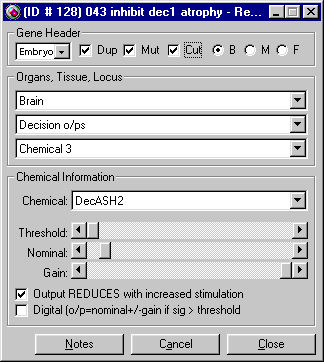
\epsfig {file=img/chemical_receptor.png,width=5.20cm}} % 11.43cm
	\caption{Interface for Chemical Receptor Design}
	\label{fig:chemical_receptor}
\end{figure}
\end{minipage}

\subsubsection{Breakdown}

\textbf{\textit{Gene Header}} : \emph{The gene header is the same for all genes. }~\\

% \textbf{\textit{Organs, Tissue, Locus}}~\\

% Defines the area of the norn that will have the result of the receptor formula applied to it. The result applied is a numeric value ranging from 0 through to 255 and its effect is different for each Locus. The following table describes what I believe to be the effects of each individual locus.~\\

%		\begin{longtable}{|p{0.15\textwidth}|p{0.20\textwidth}|p{0.65\textwidth}|}
%		\hline \rowcolor[gray]{0.50} \multicolumn{3}{|c|}{Organs, tissues, locus informations and description for Receptors} \\
%		\hline \rowcolor[gray]{0.75} \textbf{Box 1} & \textbf{Box 2} & \textbf{Box 3} \\ \hline
%		\endfirsthead
%		\hline \rowcolor[gray]{0.50} \multicolumn{3}{|c|}{Organs, tissues, locus informations and description for Receptors} \\
%		\hline \rowcolor[gray]{0.75} \textbf{Box 1} & \textbf{Box 2} & \textbf{Box 3} \\ \hline
%		\endhead
%		\hline 
%		\endfoot
%		
%			Brain & Any Brain Lobe & \textbf{Threshold} \\
%		\cline{3-3} % \hline
%				&	& Still to be investigated. If it allows adjustment to the threshold value of the given brain cell then it opens up a number of possibilities in brain modifications. The threshold is usually statically defined in the brain lobe gene - allowing it to be updated dynamically in this manner could be interesting. \\
%		\cline{3-3} % \hline
%				&	& \textbf{Leakage} \\
%		\cline{3-3} % \hline
%				&	& Still to be investigated. See the threshold comment above. \\
%		\cline{3-3} % \hline
%				&	& \textbf{Gain} \\
%		\cline{3-3} % \hline
%				&	& \emph{Still to be investigated.} \\
%		\cline{3-3} % \hline
%				&	& \textbf{Den(x) relax susceptibility} \\
%		\cline{3-3} % \hline
%				&	& \emph{Still to be investigated.} The 'x' represents the dendrite type (0 or 1). See the brain lobe section for details on dendrite types. \\
%		\cline{3-3} % \hline
%				&	& \textbf{Den(x) relax STW} \\
%		\cline{3-3} % \hline
%				&	& \emph{Still to be investigated.} \\
%		\cline{3-3} % \hline
%				&	& \textbf{Den(x) relax LTW} \\
%		\cline{3-3} % \hline
%				&	& \emph{Still to be investigated.} \\
%		\cline{3-3} % \hline
%				&	& \textbf{Den(x) strength gain rate} \\
%		\cline{3-3} % \hline
%				&	& \emph{Still to be investigated.} \\
%		\cline{3-3} % \hline
%				&	& \textbf{Den(x) strength loss rate} \\
%		\cline{3-3} % \hline
%				&	& \emph{Still to be investigated.} I believe all these Den(x) parameters allow dynamic changing of the various options available in the dendrite sections of the brain lobes. This could allow some interesting modifications to learning and reinforcement based upon external factors to the norn.\\
%		\cline{3-3} % \hline
%				&	& \textbf{Chemical n} \\
%		\cline{3-3} % \hline
%				&	& Where 'n' is a value from 0 to 3. Still to be investigated but like the above I believe it will change the amount of the particular brain chemical for the given lobe. \\
%		\cline{3-3} % \hline
%				&	& \textbf{Cell(n) State} \\
%		\cline{3-3} % \hline
%				&	& Represents the state value of the given cell in the brain lobe. See the brain lobe page for details on brain cells. \\
%
%		\hline \hline
%			Creature	&	Somatic	& \textbf{Become a child} \\
%		\cline{3-3} % \hline
%				&	& Changes the life stage of the norn to that of 'child'. The current norn genome sets this at a default value until aging chemical hits a certain level then it will drop to zero. From this I assume that a zero value indicates it has reached this particular life stage. To be investigated further. \\
%		\cline{3-3} % \hline
%				&	& \textbf{Become adolescent} \\
%		\cline{3-3} % \hline
%				&	& \emph{See above.} \\
%		\cline{3-3} % \hline
%				&	& \textbf{Become youth} \\
%		\cline{3-3} % \hline
%				&	& \emph{See above.} \\
%		\cline{3-3} % \hline
%				&	& \textbf{Become old} \\
%		\cline{3-3} % \hline
%				&	& \emph{See above.} \\
%		\cline{3-3} % \hline
%				&	& \textbf{Become senile} \\
%		\cline{3-3} % \hline
%				&	& \emph{See above.} \\
%		\cline{3-3} % \hline
%				&	& \textbf{Die of old age} \\
%		\cline{3-3} % \hline
%				&	& \emph{See above.} \\
%		\cline{3-3} % \hline
%				&	& \textbf{Become adolescent} \\
%		\cline{3-3} % \hline
%				&	& \emph{See above.} \\
%		\cline{2-3} % \hline
%				&	Circulatory	& \textbf{Floating recip-emit n} \\
%		\cline{3-3} % \hline
%				&	& A floating recip-emit is a place that a receptor can use for storing a data value from 0-255 which an emitter can then use for any purpose. It's a means of linking a receptor directly to an emitter without going through a brain lobe. There are up to eight of these numbered from 0-7 (the 'n'). The life kit norns use this for the hunger/glycogen equation. See the notes section at the end of this page for a description of this mechanism. \\
%		\cline{2-3} % \hline
%				&	Reproductive	& \textbf{Become fertile if high} \\
%		\cline{3-3} % \hline
%				&	& In the C1 genome this tracks the Oestrogen or Testosterone (Females and Males respectively) chemical exactly. To be investigated (but probably means the obvious). \\
%		\cline{3-3} % \hline
%				&	& \textbf{Receptive to sperm if >0} \\
%		\cline{3-3} % \hline
%				&	& If greater than zero then the norn is receptive to sperm. In the C1 genome it is linked to sex drive for females. From what I understand this is always greater than zero as a result of the receptor in the C1 genome. \emph{To be investigated.} \\
%		\cline{2-3} % \hline
%				&	Immune	& \textbf{Die if non-zero} \\
%		\cline{3-3} % \hline
%				&	& If the value of this is ever non-zero the norn will die. In the various life kit genomes it is linked to the aging chemical. When the chemical is lower than a certain value the norn will die. \\
%		\cline{2-3} % \hline
%				&	Sensorimotor	& \textbf{Involuntary Action n} \\
%		\cline{3-3} % \hline
%				&	& Where 'n' is a number from 0 through to 7. Activates the particular involuntary action. \emph{To be investigated.} \\
%		\cline{3-3} % \hline
%				&	& \textbf{<normal walk gait (do not use)>} \\
%		\cline{3-3} % \hline
%				&	&  \emph{To be investigated.} \\ 
%		\cline{3-3} % \hline
%				&	& \textbf{Special gait n} \\
%		\cline{3-3} % \hline
%				&	&  Where 'n' is a number from 1 through to 7. \emph{To be investigated.} \\
%		\cline{2-3} % \hline
%				&	Drive Levels	& \textbf{Drive Lobe} \\
%		\cline{3-3} % \hline
%				&	& Allows setting of the drive level for a norn. In the C1 genome this is set to match the particular drive chemical exactly. \\
%		\hline
%	\caption{Organs, tissues, locus informations and description for Receptors}
%	\label{tab:Receptor_OrganTissuesLocus}\\
%	\end{longtable}

\textbf{\textit{Chemical Information}}
\begin{itemize}
	\item[] \emph{Chemical} : Defines the particular chemical that will be monitored. %  by the receptor
	\item[] \emph{Threshold} : Defines the level of the chemical that must exist before the given locus is activated. In the case of Digital receptors the amount of chemical must be greater than this threshold before the locus is activated. For Analogue receptors the signal (ie. amount of chemical) is reduced by the amount of this threshold before calculating the amount to stimulate the locus by. See Formula below for the calculation used.
	\item[] \emph{Nominal} : Defines the default or base value used to stimulate the locus. This what the locus will be set to if the amount of chemical is not greater than the threshold. 
	\item[] \emph{Gain} : Defines what the value of the locus will be set to in the case of a digital receptor or as a scaling factor for calculating the amount in an analog receptor. See Formula below for details.
	\item[] \emph{Output REDUCES with increased stimulation} : If this is checked then all adjustments to the base value of the receptor (ie. the Nominal amount) will reduce that base value. If cleared all adjustments will increase the base value.
	\item[] \emph{Digital} : The locus will be set to a constant amount if the chemical amount is greater than a certain threshold if this option is checked. If it is unchecked then the receptor is analogue. This means that the locus will be set to a value in proportion to the amount of chemical. See below for details.
\end{itemize}

\textbf{\textit{Formula}}

\underline{Analogue receptors} formula for calculating the value for the locus:

$Nominal + (((ChemicalAmount - Threshold) * Gain/255) * R)$

Where R is 1 if 'Output Reduces with increased stimulation' is not checked and -1 if it is checked. So the nominal will be reduced or increased based upon this flag.~\\

\underline{Digital receptors} formula for calculating the value for the locus:

$Nominal + ((ChemicalAmount > Threshold ? Gain : 0) * R)$

So if the chemical amount is greater than the threshold then the locus setting will be the Nominal amount increased or decreased by the Gain depending on the setting of 'R'. If it is not greater than the threshold then the locus setting will be equivalent to Nominal.~\\

% \subsubsection{Notes}
% I've found that the norn genome has become much clearer to me now that I understand exactly how the receptor is calculated. And the possibility of dynamically modifying the various settings of the brain lobes leads to some interesting areas as well.~\\
% Using the information above I examined how the new hunger/glycogen reaction works in the life kit norns. Using a receptor the glycogen chemical is attached to floating recep-emitter number 2 (FRE-2). The settings for this emitter make FRE-2 exactly equal to the amount of glycogen chemical. So a value of 100 glycogen will cause a value of 100 FRE-2.~\\
% The hunger emitter gets it's input from FRE-2. It is an analogue emitter with a sample rate of 5, a gain of 2, a threshold of zero and it is inverted.~\\
% This means that approximately every half second or so the hunger chemical is increased by an amount equal to:~\\
% $(255 - GlycogenAmount) * 2/255$~\\
% So high glycogen means that hunger will not be increased. Glycogen has to be lower than about 100 before hunger is adjusted to any great degree. So if you don't want your norns to be hungry, keep their glycogen levels high.~\\

%%%%%%%%%%%%%%%%%%%%%%%%%%%%%%%%%%%%%%%%%%%%%%%%%%%%%%%%%%%%%%%
% % % % % % demi-vie
% \subsection{CDR -- Chemical Half-Life}

% \begin{minipage}{0.5\linewidth}
% \subsubsection{Overview}
% The chemical half-life gene defines the decay rate of all the chemicals inside a norn. Each chemical has a value ranging from 0 through to 255 representing the amount of substance within the norn. The higher the number the more chemical inside the norn.~\\
% To prevent the chemical from staying permanently within the norn you can set a decay rate. This sets a period of time over which the chemical amount will slowly drop down towards zero.
% \end{minipage}
% \begin{minipage}{0.1\linewidth}\end{minipage}
% \begin{minipage}{0.4\linewidth}
% \subsubsection{Dialog Box}
% \begin{figure}[H]
% 	\centerline {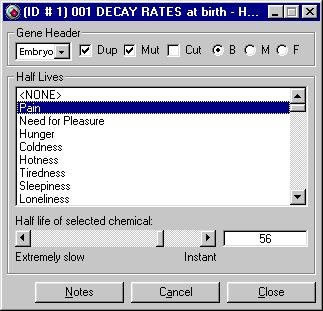
\epsfig {file=img/chemical_halflife.png,width=5.20cm}} % 11.40cm
% 	\caption{Interface for Chemical Half Lives Design}
% 	\label{fig:chemical_halflife}
% \end{figure}
% \end{minipage}
% \subsubsection{Breakdown}
% \textbf{\textit{Gene Header}} : \emph{The gene header is the same for all genes.}~\\
% \textbf{\textit{Half Lives}}~\\
% \begin{itemize}
% \item[] \textit{Chemical}~\\
%     Within this listbox you can select any of the 255 different chemicals that may exist within the Norn. The selected chemical will be the one that the rate of decay can be defined for in the controls below this listbox.
% \item[] \textit{Half Life}~\\
%     This defines the rate at which the selected chemical will decay. It is a number ranging from 0 through to 255. The higher the number the longer it takes for the chemical to drop down to zero. The Genetics Kit only allows certain numbers to be selected and for these numbers it displays an approximate time in seconds.~\\
% This is the time it will take for the chemical to drop from it's value down to zero. The following table shows the number and approximate rate as listed by the genetics kit:
% \end{itemize}
%\begin{longtable}{|p{0.075\textwidth}|p{0.20\textwidth}|p{0.001\textwidth}|p{0.075\textwidth}|p{0.20\textwidth}|}
%	\hline \rowcolor[gray]{0.50} \multicolumn{5}{|c|}{Half lives of chemicals} \\
%	\hline \rowcolor[gray]{0.75} \textbf{Half Life} & \textbf{Approximate Time} & & \textbf{Half Life} & \textbf{Approximate Time} \\ \hline
%	\endfirsthead
%	\hline \rowcolor[gray]{0.50} \multicolumn{5}{|c|}{Half lives of chemicals} \\
%	\hline \rowcolor[gray]{0.75} \textbf{Half Life} & \textbf{Approximate Time} & & \textbf{Half Life} & \textbf{Approximate Time} \\ \hline
%	\endhead
%	\hline 
%	\endfoot
%
%	0 	&	Instantly	 & &	128 &	5 hours \\ \hline
%	8 	&	0.4 seconds	 & &	136 &	10 hours \\ \hline
%	16 	&	1 second	 & &	144 &	20 hours \\ \hline
%	24 	&	3 seconds	 & &	152 &	3 days \\ \hline
%	32 	&	5 seconds	 & &	160 &	6 days \\ \hline
%	40 	&	10 seconds	 & &	168 &	12 days \\ \hline
%	48 	&	20 seconds	 & &	176 &	24 days \\ \hline
%	56 	&	40 seconds	 & &	184 &	48 days \\ \hline
%	64 	&	80 seconds	 & &	192 &	96 days \\ \hline
%	72 	&	2.5 minutes	 & &	200 &	112 days \\ \hline
%	80 	&	5 minutes	 & &	208 &	224 days \\ \hline
%	88 	&	10 minutes	 & &	216 &	448 days \\ \hline
%	96 	&	20 minutes	 & &	224 &	896 days \\ \hline
%	104 &	40 minutes	 & &	232 &	13 years \\ \hline
%	112 &	80 minutes	 & &	240 &	26 years \\ \hline
%	120 &	2.5 hours	 & &	248 &	52 years \\ \hline
%	
%		\hline
%	\caption{Half lives of chemicals}
%	\label{tab:Half_lives_chemicals}\\
%\end{longtable}~\\

%\subsubsection{Notes}
%I'm assuming by the name of the gene that the rate represents a half-life. So it defines the time it takes for the chemical to drop to half of its current value. It seems to work in this manner anyway.~\\
%\rule{10cm}{0.5mm}~\\

% \clearpage

\subsection{Initial Concentrations} % CDR -- 
\begin{minipage}{0.5\linewidth}
\subsubsection{Overview}
This gene controls the amount of chemical that will exist within the norn when it is born (or when the gene is activated?). One gene of this kind exists for each chemical within the norn that requires an initial starting value. I don't know the effects of changing the 'switch on' age. If the age is set to something other than embryo does this mean that an amount of chemical will be injected when the creature reaches that age?~\\
\end{minipage}
\begin{minipage}{0.1\linewidth}\end{minipage}
\begin{minipage}{0.4\linewidth}
\subsubsection{Dialog Box}
\begin{figure}[H]
	\centerline {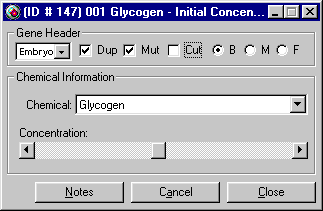
\epsfig {file=img/chemical_initial.png,width=5.20cm}} % 11.40cm
	\caption{Interface for Initial Concentration Design}
	\label{fig:chemical_initial}
\end{figure}
\end{minipage}

\subsubsection{Breakdown}

\textbf{\textit{Gene Header}} : \emph{The gene header is the same for all genes.}~\\

\textbf{\textit{Chemical Information}}
\begin{itemize}
	\item[] \emph{Chemical} : This will be the chemical that will have the initial concentration defined for this gene.
	\item[] \emph{Concentration} : The amount of chemical to be initially injected into the norn. It is a value from 0 through to 255.
\end{itemize}

\rule{10cm}{0.5mm}~\\

\subsection{Creature Instinct} % CDR -- 

\subsubsection{Overview}

An instinct gene provides a way of training the neural net of the norn brain so it will react in certain ways in certain situations. Instinct genes are often used to provide default behavior for things that are very important to the norn. Examples are responding to the verbs typed by the user. These genes do not provide behavior that will always occur. The experiences of the norn during its lifetime can override behavior defined by instincts.~\\

Instincts are processed while a norn is being hatched and while a norn sleeps. It is very important for a norn to get regular sleep so the instincts are constantly reinforced. During this instinct processing time the lobes and neurones define in the gene are set inside the norn brain and the chemical (usually punishment or reward) is processed as if the norn had performed this action.~\\

For example the instinct gene responding to the verb 'come' has the same effect when processed as if the norn had chosen the decision to 'come' when the user typed 'come' and then got a pat from the hand to reward it. This would encourage the norn to do this when awake.

\clearpage

\subsubsection{Dialog Box}

\begin{figure}[H]
	\centerline {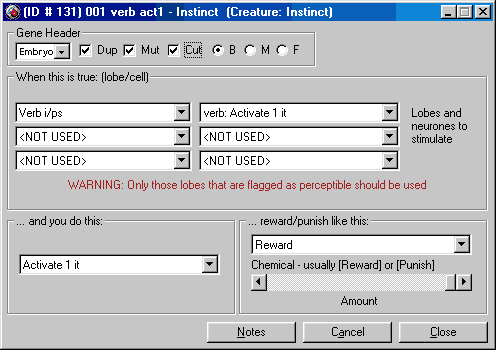
\epsfig {file=img/genes_instinct.png,width=8.75cm}} % 17.498cm
	\caption{Interface for Intincts Design}
	\label{fig:genes_instinct}
\end{figure}

\subsubsection{Breakdown}

\textbf{\textit{Gene Header}} : \emph{The gene header is the same for all genes.}~\\

\textbf{\textit{When this is true: (lobe/cell)}}~\\

Allows selection of the lobes and cells that will be fired within those lobes. This indicates what the norn will need to perceive before it will decide to take the action defined in the 'and you do this' area. A combination of up to three different lobe/cells may be selected. The Genetics Kit gives a warning that only those lobes marked as perceptible should be used. This makes sense as only the perceptible lobes contribute to forming concepts. Any other lobe will cause this instinct to have no real effect.~\\

The lobes and their perceptible settings are:
\begin{longtable}{|p{0.30\textwidth}|p{0.50\textwidth}|}
	\hline \rowcolor[gray]{0.50} \multicolumn{2}{|c|}{Lobes and perceptible settings} \\
	\hline \rowcolor[gray]{0.75} \textbf{Lobe} & \textbf{Perceptible setting} \\ \hline
	\endfirsthead
	\hline \rowcolor[gray]{0.50} \multicolumn{2}{|c|}{Lobes and perceptible settings} \\
	\hline \rowcolor[gray]{0.75} \textbf{Lobe} & \textbf{Perceptible setting} \\ \hline
	\endhead
	\hline 
	\endfoot

		Drive i/ps 			&	Mutually exclusive 	\\ \hline
		Stim source i/ps 	&	No 					\\ \hline
		Verb i/ps 			&	Mutually exclusive 	\\ \hline
		Noun i/ps 			&	No 					\\ \hline
		Gen/sense i/ps 		&	Yes 				\\ \hline
		Decision 			&	No 					\\ \hline
		Attention 			&	Yes 				\\ \hline

	\hline
	\caption{Lobes and perceptible settings}
	\label{tab:Lobes_and_perceptible_settings}\\
\end{longtable}~\\~\\

All lobes with a perceptible setting of 'Yes' or 'Mutually Exclusive' qualify as perceptible lobes so they should be able to be used in instincts.~\\

\textbf{\textit{and you do this...}}~\\
This is the decision that the instinct will reinforce when the above lobe/cell combinations are active. Think of it as 'if the above lobe combinations occur then the norn will be more or less likely to make this decision depending on the reward/punish settings defined below. \emph{Valid settings are any of the 16 possible decisions or verbs that the norn can perform: }
	\begin{center} \begin{scriptsize}
		\begin{tabular}{|p{0.5\textwidth}|p{0.5\textwidth}|}
			\hline
			\begin{enumerate}
				\item[0.] Default (\textbf{Stay})
				\item[1.] Activate 1 it (\textbf{Push})
				\item[2.] Activate 2 it (\textbf{Pull})
				\item[3.] Deactivate it (\textbf{Stop})
				\item[4.] Approach it (\textbf{Come})
				\item[5.] Retreat from it (\textbf{Run})
				\item[6.] Get it (\textbf{Get})
				\item[7.] Drop all (\textbf{Drop})
			\end{enumerate}
			&
			\begin{enumerate}
				\item[8.] Say what you need (\textbf{Think})
				\item[9.] Rest (\textbf{Sleep})
				\item[10.] Travel west (\textbf{Left})
				\item[11.] Travel east (\textbf{Right})
				\item[12.] Decision12
				\item[13.] Decision13
				\item[14.] Decision14
				\item[15.] Decision15
			\end{enumerate} \\ \hline
		\end{tabular}
	\end{scriptsize} \end{center}~\\

\textbf{\textit{reward/punish like this}}~\\
This is where you select the chemical and amount of that chemical that will be injected into the norn when the above settings are made and the instinct processed. Although any of the 256 chemicals can be selected the only two that really make sense are 'Reward' or 'Punish'.~\\

If 'Reward' is selected then the norn will be rewarded and encouraged to perform the action. If 'Punish' is selected then the norn will be discouraged and be less likely to perform the action defined.

\subsubsection{Notes}

Remember that instincts are only processed when a norn is born and while it sleeps. Too many instinct genes could cause a lot more sleep or longer sleep to be required for all the instincts to be processed. It may pay to have the more important instincts to be the lower numbered genes (as it appears to cycle through in gene number order).~\\

Some instinct genes appear to use the Stim source lobe as an input even though it is not a perceptible lobe. I'm in the process of testing whether these instincts actually work as I suspect they may not. It depends whether the instinct processing mechanism still considers it as perceptible as the Stim source lobe feeds into the Attention lobe which is perceptible. Some research is needed here.~\\

Although only 'Reward' and 'Punish' currently make sense for chemicals, others could be useful in genetically modified norns with different brain/chemical structures. There is scope for some interesting experimentation there. Only three lobe/cell combinations can be defined. This appears to match the number of dendrite links between the perception lobe and the concept lobe in a standard hatchery norn. These norns allow up to three perceptions to form a concept.~\\

% If you can provide any additional information to help document this gene please let me know (chris@double.co.nz).~\\

% \rule{10cm}{0.5mm}~\\

\subsection{Creature Stimulus} % CDR -- 
\begin{minipage}{0.5\linewidth}
\subsubsection{Overview}
A stimulus is an event that happens to the norn that it can react to in some manner. The stimulus gene allows the reaction to these stimuli to be defined. This can range from chemicals being injected to cell values in brain lobes being adjusted. There are a number of stimulus responses that are hard coded within the Creatures program. The stimulus genes that are created override these hard coded responses giving a lot of flexibility in determining how the creature will react to the world.~\\
\end{minipage}
\begin{minipage}{0.1\linewidth}\end{minipage}
\begin{minipage}{0.4\linewidth}
\subsubsection{Dialog Box}
\begin{figure}[H]
	\centerline {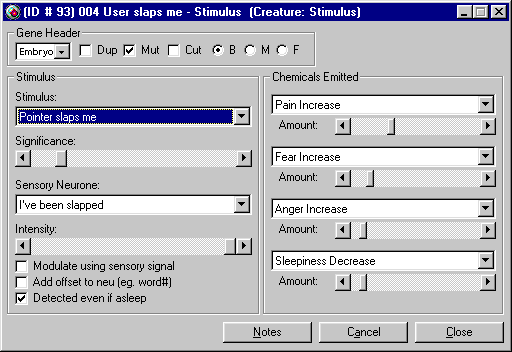
\epsfig {file=img/gene_stimulus.png,width=5cm}} % 18.00cm
	\caption{Interface for Stimulus Design}
	\label{fig:genes_stimulus}
\end{figure}
\end{minipage}~\\

\clearpage

\subsubsection{Breakdown}

\textbf{\textit{Gene Header}} : \emph{The gene header is the same for all genes.}~\\

\textbf{\textit{Stimulus}}
\begin{itemize}
\item[] \emph{Stimulus} : The stimulus that this gene is attached to. When this stimulus occurs then the effects defined by this gene will be applied. The following stimuli are available:
	\begin{center} \begin{scriptsize}
		\begin{tabular}{|p{0.30\textwidth}|p{0.30\textwidth}|p{0.30\textwidth}|}
			\hline
			\begin{itemize}
				\item Disappointment
				\item Pointer pats me
				\item Creature pats me
				\item Pointer slaps me
				\item Creature slaps me
				\item It is approaching
				\item It is retreating
				\item I bump into wall
				\item Object comes into view
			\end{itemize}
			&
			\begin{itemize}
				\item Unrecognised word
				\item Heard user speak
				\item Heard creature speak
				\item I am quiescent (periodic)
				\item I've activated1
				\item I've activated2
				\item I've deactivated
				\item I am approaching (periodic)
				\item I have retreated
			\end{itemize}
			&
			\begin{itemize}
				\item I have got
				\item I have dropped
				\item I've stated need
				\item I am resting (periodic)
				\item I am sleeping (periodic)
				\item I am traveling (periodic)
				\item spare action 1-4
				\item Involuntary action 0-7
			\end{itemize} \\ \hline
		\end{tabular}
	\end{scriptsize} \end{center}~\\
 
\item[] \emph{Significance} : The amount will be increased the neuron relating to the object that caused the stimulus in the Stimulus/Source lobe. This has the effect of making the object appear more interesting and so it is more likely to be looked at. The neuron that gets nudged by this amount appears to differ for each Stimuli (a neuron for each object type in view). 
\item[] \emph{Sensory Neurone} : Identifies a cell in the General Sense lobe which will get adjusted by the value given in the 'Intensity' field described below. This allows setting up what the norn can actually sense from the stimuli going on around it. The following cells are available and map directly to cells in the general sense lobe:
	\begin{center} \begin{scriptsize}
\begin{tabular}{|p{0.30\textwidth}|p{0.30\textwidth}|p{0.30\textwidth}|}
		\hline
			\begin{itemize}
				\item $<$none$>$
				\item I've been patted
				\item I've been slapped
				\item I've bumped a wall
				\item I am near a wall
				\item I am in a vehicle
				\item User has spoken
				\item Creature has spoken
			\end{itemize}
			&
			\begin{itemize}
				\item Own kind has spoken
				\item Audible event
				\item Visible event
				\item It is approaching
				\item It is retreating
				\item It is near to me
				\item It is active
			\end{itemize}
			&
			\begin{itemize}
				\item It is an object
				\item It is a creature
				\item It is my sibling
				\item It is my parent
				\item It is my child
				\item It is opposite sex
				\item spare 2-13
			\end{itemize} \\
		\hline
		\end{tabular}
	\end{scriptsize} \end{center}~\\
 
\item[] \emph{Intensity} : This is the amount by which the particular sensory neurone will be increased by. So if the value here is '50' and the current value of the particular neurone is '25' then when this stimuli occurs the sensory neurone will fire at a value of about '75'.
\item[] \emph{Modulate using sensory signal} : From what I can gather this means that the 'significance' value applied to the stimulus source lobe is first modulated by the value of the neuron associated with the stimulus. I'm not exactly sure what particular value it is modulated by and perhaps it is best explained by describing some of the results I've gotten through experimentation. See the notes section for details. If anyone can provide a clearer explanation I'd appreciate an email.
% \item[] \emph{Add offset to neu (eg. word\#)} : 
\item[] \emph{Detected even if asleep} : If the norn is asleep and this option is unchecked then the stimulus will be ignored and none of the effects will be applied. If it is checked then the gene will be processed even if the norn is sleeping.
\end{itemize}~\\

\textbf{\textit{Chemicals Emitted}}~\\
Up to four chemicals can be selected along with a particular amount of that chemical to be injected. When the stimulus occurs the defined amount of these chemicals will be injected into the norn.

\clearpage

%%%%% \subsection{CDR -- State Variable Rules (SVR)}

\subsection{Brain Lobes -- \textit{Creatures 1}} % CDR -- 

% $<$\textit{http://www.double.co.nz/creatures/brainlobes/lobes.htm}$>$

\subsubsection{Overview}

The norn brain is divided into a number of lobes. In the standard Creatures 1 genome there are nine and in the Creatures 2 genome there are ten.~\\

The brain lobes numbered from 0 through to 8 are hard coded by the Creatures executable to perform a particular function. For example, firing a cell in lobe 6 (decision) causes the creature to perform a particular action. The genetic definition of that lobe then defines what happens as a result of this firing. In the case of the decision lobe it is to manage the learning of whether the decision was a good one or a bad one.~\\

The higher numbered brain lobes are not controlled by the Creatures executable at all. They are controlled completely through genetics. So for these lobes to do anything a system of receptors, emitters and dendrites must be set up to fire cells or act upon cells firing.~\\

The purpose and function of each lobe is outlined below with descriptions.
\begin{itemize}
\item[\textbf{Lobe 0 -- Perception}]
    Copies data from other lobes to form a composite lobe containing all cells that can be used to form concepts.
\item[\textbf{Lobe 1 -- Drive}]
    Holds the current values of the creatures drives.
\item[\textbf{Lobe 2 -- Stimulus source}]
    Stimulating objects near to the creature cause cells in this lobe to fire so the creature can react to them.
\item[\textbf{Lobe 3 -- Verb}]
    Cells in this lobe fire when the user types a verb in the speech box.
\item[\textbf{Lobe 4 -- Noun}]
    Cells in this lobe fire when the user types a noun in the speech box or types 'look' with the hand hovering over an object.
\item[\textbf{Lobe 5 -- General Sensory}]
    Indicates events that the norn can sense. Usually caused by the effects of processing stimulus genes.
\item[\textbf{Lobe 6 -- Decision}]
    An output lobe. By firing a cell in this lobe you cause the creature to perform a particular action.
\item[\textbf{Lobe 7 -- Attention}]
    An output lobe. By firing a cell in this lobe you cause the creature to look at a particular object.
\item[\textbf{Lobe 8 -- Concept}]
    A storehouse of memories and concepts.
\item[\textbf{Lobe 9 -- Regulator}]
    This lobe provides feedback loops for biochemical regulations. % This lobe is not really part of the norn brain/decision mechanism as such. It provides functionality similar to the hunger/glycogen floating receptor emitters used by the norns in the Creatures 1 life kit. Special thanks to Lis Morris for the description of this lobe.
\end{itemize}~\\

While the lobes have individual functionality it is how they work together that results in the norn brain working. There lobes combine to form a couple of main learning systems that are described briefly in the individual lobe descriptions but will be covered in more detail in future updates:
\begin{itemize}
	\item Attention seeking system
	\item Concept learning system
	\item Decision learning system
\end{itemize}~\\


%% \def\captionof#1#2{{\def\@captype{#1}#2}}
%% attention aux flottants dans les flottants !!
\begin{table}[ht]
	\begin{center} \begin{scriptsize}
	\begin{tabular}{|c|c|c|c|c|c|c|}
		\hline
	\rowcolor[gray]{0.75} 
	Number	&	Name	&	X	&	Y	&	Width	&	Height	&	Neurones \\ \hline
	0	&	Perception	&	4	&	13	&	7		&	16		&	112 \\ \hline
	1	&	Drive		&	34	&	30	&	8		&	2		&	16 \\ \hline
	2	&	Source		&	15	&	24	&	8		&	5		&	40 \\ \hline
	3	&	Verb		&	37	&	24	&	8		&	2		&	16 \\ \hline
	4	&	Noun		&	21	&	3	&	20		&	2		&	40 \\ \hline
	5	&	Gen. Sense	&	32	&	34	&	8		&	4		&	32 \\ \hline
	6	&	Decision	&	53	&	15	&	1		&	16		&	16 \\ \hline
	7	&	Attention	&	44	&	30	&	5		&	8		&	40 \\ \hline
	8	&	Concept		&	12	&	6	&	40		&	16		&	640 \\ \hline
	\end{tabular}
	\caption[Norn Lobes for \emph{Creatures 1}]{Norn Lobes for \emph{Creatures 1} \\ \emph{Description of lobes positions and size,  brain is $64*48$. The Regulator lobe, \textnormal{SandraBellum}, is not present~\cite{genornics}. } }
	\end{scriptsize} \end{center}
	\label{tab:nornsLobesPositionsCreatures1}
\end{table}



\begin{table}[ht]
	\begin{center} \begin{scriptsize}
	\begin{tabular}{|c|c|c|c|c|c|c|}
		\hline
	\rowcolor[gray]{0.75} 
	Number	&	Name	&	X	&	Y	&	Width	&	Height	&	Neurones \\ \hline
	0	&	Perception	&	1	&	13	&	7		&	16		&	112 \\ \hline
	1	&	Drive		&	34	&	36	&	6		&	3		&	18 \\ \hline
	2	&	Source		&	15	&	32	&	8		&	5		&	40 \\ \hline
	3	&	Verb		&	37	&	32	&	8		&	2		&	16 \\ \hline
	4	&	Noun		&	21	&	1	&	20		&	2		&	40 \\ \hline
	5	&	Gen. Sense	&	32	&	40	&	8		&	4		&	32 \\ \hline
	6	&	Decision	&	62	&	15	&	1		&	16		&	16 \\ \hline
	7	&	Attention	&	44	&	36	&	5		&	8		&	40 \\ \hline
	8	&	Concept		&	11	&	5	&	40		&	16		&	640 \\ \hline
	9	&	Regulator	&	4	&	40	&	16		&	1		&	16 \\ \hline
	\end{tabular}
	\end{scriptsize} \end{center}
	\caption[Norn Lobes for \emph{Creatures 2}]{Norn Lobes for \emph{Creatures 2} \\ \emph{Description of lobes positions and size,  brain is $64*48$~\cite{genornics}. } }
	\label{tab:nornsLobesPositionsCreatures2}
\end{table}


\begin{minipage}{0.5\textwidth}
\begin{figure}[H]
	\centerline {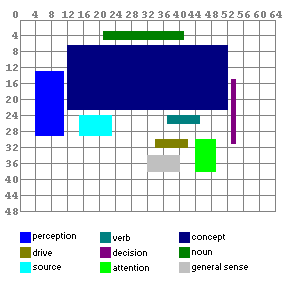
\epsfig {file=img/brainmapCreatures1.png,width=7cm}}
	\caption{Creatures 1 Brain Map~\cite{genornics}}
	\label{fig:Creatures1BrainMap}
\end{figure}
\end{minipage}
\begin{minipage}{0.1\textwidth}\end{minipage}
\begin{minipage}{0.5\textwidth}
\begin{figure}[H]
	\centerline {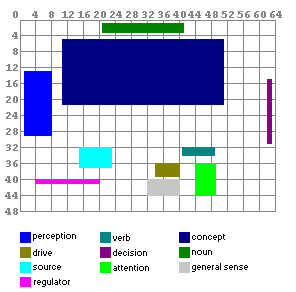
\epsfig {file=img/brainmapCreatures2.png,width=7cm}}
	\caption{Creatures 2 Brain Map~\cite{genornics}}
	\label{fig:Creatures2BrainMap}
\end{figure}
\end{minipage}

% \clearpage

\subsubsection{Lobe 0 -- Perception Lobe}

% \emph{To be completed. \underline{see special section} }

The purpose of the perception lobe appears to be to summarise everything that a norn can 'perceive' into one brain lobe so the norn can eventually store concepts and memories based upon these perceptions (done in the concept lobe). This tutorial attempts to answer the questions about how the perceptible lobes are summarised into the perception lobe and how to work out what each cell of the perception lobe means.~\\

The usual method of passing cell information from one lobe to another is through wiring up dendrites. Using dendrites can only summarise information from two other brain lobes (the D0 and D1 dendrite connections). With the perception lobe there is more than two lobes that need to be summarised so it appears a mechanism specifically for dealing with the perception lobe was built.~\\

Brain lobes are marked as 'Yes', 'No' or 'Mutually Exclusive' to be copied in the Perception lobe. The brain lobes that are marked as 'Yes' or 'Mutually exclusive' in an original norn are:
\begin{longtable}{|p{0.25\textwidth}|p{0.15\textwidth}|p{0.65\textwidth}|}
	\hline \rowcolor[gray]{0.50} \multicolumn{3}{|c|}{Copied Lobes in Perception} \\
	\hline \rowcolor[gray]{0.75} \textbf{Lobe} & \textbf{Size} & \textbf{Data copied to perception lobe?} \\ \hline
	\endfirsthead
	\hline \rowcolor[gray]{0.50} \multicolumn{3}{|c|}{Copied Lobes in Perception} \\
	\hline \rowcolor[gray]{0.75} \textbf{Lobe} & \textbf{Size} & \textbf{Data copied to perception lobe?} \\ \hline
	\endhead
	\hline 
	\endfoot
	Drive lobe		&	16 &	Mutually exclusive \\ \hline
	Verb lobe		&	16 &	Mutually exclusive \\ \hline
	General sense lobe	&	32 &	Yes \\ \hline
	Attention lobe 		&	40 &	Yes \\ \hline
	\caption{Copied Lobes in Perception}
	\label{tab:Copied_Lobes_in_Perception}\\
\end{longtable}

\clearpage

The perception lobe must have a number of cells equal to or greater than the total number of cells in all lobes marked as 'Yes' or 'Mutually exclusive'. The total number of cells in the above lobes equals 104. The size of the perception lobe is 112 so there is a little room to spare there.

\subsubsection{Lobe 1 -- Drive Lobe}

This lobe holds the current state of the creatures drives (such as hunger, pain, etc). It directly maps to the particular drive chemicals that can be viewed using the science kit. Changing the values of the cells directly in this lobe using CAOS is unlikely to have much of an effect on the norn as the cells are directly set by receptors in the genome. This means that whatever values you manipulate with CAOS commands will be immediately overwritten with the current value of the drive chemical. To change drive values it would seem to be best to change the values of the chemicals either directly or through the drive increaser/reducer chemicals. \emph{The size of the lobe was increased in Creatures 2 to cater for the addition of more drives. The cell values are outlined in the following table:}
\begin{longtable}{|p{0.15\textwidth}|p{0.40\textwidth}|p{0.40\textwidth}|}
	\hline \rowcolor[gray]{0.50} \multicolumn{3}{|c|}{Drive Lobe Data Entries \textit{Drives} } \\
	\hline \rowcolor[gray]{0.75} \textbf{Cell} & \textbf{Creatures 1} & \textbf{Creatures 2} \\ \hline
	\endfirsthead
	\hline \rowcolor[gray]{0.50} \multicolumn{3}{|c|}{Drive Lobe Data Entries \textit{Drives} } \\
	\hline \rowcolor[gray]{0.75} \textbf{Cell} & \textbf{Creatures 1} & \textbf{Creatures 2} \\ \hline
	\endhead
	\hline 
	\endfoot

0	&	Pain			&	Pain			 \\ \hline
1	&	Need for Pleasure	&	Need for Pleasure	 \\ \hline
2	&	Hunger			&	Hunger			 \\ \hline
3	&	Coldness		&	Coldness		 \\ \hline
4	&	Hotness			&	Hotness			 \\ \hline
5	&	Tiredness		&	Tiredness		 \\ \hline
6	&	Sleepiness		&	Sleepiness		 \\ \hline
7	&	Loneliness		&	Loneliness		 \\ \hline
8	&	Overcrowdedness		&	Overcrowdedness		 \\ \hline
9	&	Fear			&	Fear			 \\ \hline
10	&	Boredom			&	Boredom	 		 \\ \hline
11	&	Anger			&	Anger	 		 \\ \hline
12	&	Sexdrive		&	Sexdrive		 \\ \hline
13	&	\emph{Not Allocated}	&	Injury	 		 \\ \hline
14	&	\emph{Not Allocated}	&	Suffocation		 \\ \hline
15	&	\emph{Not Allocated}	&	Thirst			 \\ \hline
16	&	\emph{No such cell}	&	Stress			 \\ \hline
17	&	\emph{No such cell}	&	\emph{Not Allocated}	 \\ \hline
	\caption{Drive Lobe Data Entries \textit{Drives} }
	\label{tab:Drive_Lobe_Data_Entries}\\
\end{longtable}

The drive lobe feeds into the Perception lobe and is marked as mutally exclusive. This means that, at most, one cell from the drive lobe will exist in any given concept that the creature forms. So the creature cannot form the concept of 'hot and hungry'. Only 'hot' or 'hungry' or a combination of these drives with some other perception lobe cell. 

\subsubsection{Lobe 2 -- Stimulus Source Lobe}

Cells in this lobe are activated directly by the Creatures executable. The lobe has 40 cells - one for each object classification in Creatures. -- Each cell relates to a particular object classification. The cell fires for a given object if that object is within the creatures line of sight and is stimulating in some manner. Stimulus genes can be used to modify this lobe indirectly to indicate whether the object is more or less stimulating. The higher the cell value in a particular cell, the more stimulating that object currently is.~\\

It is a 'winner takes all' lobe, meaning that the highest firing cell will be the only firing cell. This means that the most stimulating object in the area of the norn will be the only object that will appear to be stimulating to the norn. The State value for all the cells is calculated and the cell with the highest state will be the only one with an output value - indicating that it is firing.~\\

% In Creatures 1 this lobe has no state variable rule indicating that the state values are directly set by the executable or some other means (like cobs or genetics).~\\

% In Creatures 2 there is a state variable rule set to '$random:0:chem 5:PLUS:state:end$'. This means that the state is calculated by getting the previous state value and adding a random number (ranging from 0 through to the value of chemical 5) to it. Brain chemical 5 is set via a receptor gene that reacts to the chemical Triptophan (169). This receptor injects brain chemical 5 at the same level as the Triptophan chemical exists in the norn. Triptophan is described in the strategy guide as causing creatures to see objects that are not really there - a hallucinogenic. This state rule is how it works. If an amount of 100 units of Triptophan exists in the norn then 100 units of brain chemical 5 will exist. This will cause all cells in the stimulus source lobe to have their state calculated as the previous state plus a random number from 0 to 100. So the creature can end up thinking things are there when they are really not.~\\

% \rule{10cm}{0.5mm}~\\~\\

The following table outlines the cell values for this lobe:
\begin{longtable}{|p{0.15\textwidth}|p{0.40\textwidth}|p{0.40\textwidth}|}
	\hline \rowcolor[gray]{0.50} \multicolumn{3}{|c|}{Source Lobe Data Entries} \\
	\hline \rowcolor[gray]{0.75} \textbf{Cell} & \textbf{Creatures 1} & \textbf{Creatures 2} \\ \hline
	\endfirsthead
	\hline \rowcolor[gray]{0.50} \multicolumn{3}{|c|}{Source Lobe Data Entries} \\
	\hline \rowcolor[gray]{0.75} \textbf{Cell} & \textbf{Creatures 1} & \textbf{Creatures 2} \\ \hline
	\endhead
	\hline 
	\endfoot
	
0	&	Current norn		&	Current norn	 \\ \hline
1	&	Hand			&	Hand		 \\ \hline
2	&	Call button		&	Call Button	 \\ \hline
3	&	Water			&	Nature	 	 \\ \hline
4	&	Plant			&	Plant		 \\ \hline
5	&	Egg			&	Egg		 \\ \hline
6	&	Food			&	Food		 \\ \hline
7	&	Drink			&	Drink		 \\ \hline
8	&	Vendor			&	Dispenser	 \\ \hline
9	&	Music			&	Implement	 \\ \hline
10	&	Animal			&	Cliff Edge	 \\ \hline
11	&	Fire			&	Detritus	 \\ \hline
12	&	Shower			&	Medicine	 \\ \hline
13	&	Toy			&	Toy	 	 \\ \hline
14	&	Bigtoy			&	Weather	 	 \\ \hline
15	&	Weed			&	Badplant	 \\ \hline
16	&	Incubator		&	Nest		 \\ \hline
17	&	Blackboard word 33	&	Badbug		 \\ \hline
18	&	Blackboard word 34	&	Bug		 \\ \hline
19	&	Blackboard word 35	&	Badcritter	 \\ \hline
20	&	Blackboard word 36	&	Critter		 \\ \hline
21	&	Blackboard word 37	&	Seed		 \\ \hline
22	&	Blackboard word 38	&	Leaf		 \\ \hline
23	&	Blackboard word 39	&	Root		 \\ \hline
24	&	Blackboard word 40	&	Flower		 \\ \hline
25	&	Blackboard word 41	&	Fruit		 \\ \hline
26	&	Mover			&	Mover		 \\ \hline
27	&	Lift			&	Lift		 \\ \hline
28	&	Computer		&	Computer	 \\ \hline
29	&	Fun			&	Mediabox	 \\ \hline
30	&	Bang			&	Message		 \\ \hline
31	&	Blackboard word 47	&	Leftright	 \\ \hline
32	&	Blackboard word 48	&	Incubator	 \\ \hline
33	&	Blackboard word 49	&	Teleporter	 \\ \hline
34	&	Blackboard word 50	&	Blackboard word 50	 \\ \hline
35	&	Blackboard word 51	&	Machine		 \\ \hline
36	&	Norn			&	Norn		 \\ \hline
37	&	Grendel			&	Grendel		 \\ \hline
38	&	Ettin			&	Ettin		 \\ \hline
39	&	Shee			&	Shee		 \\ \hline

		\hline
	\caption{Source Lobe Data Entries }
	\label{tab:Source_Lobe_Data_Entries}\\
\end{longtable}

The cell numbers appear to relate to the genus numbers for Objects (COB). So an Object with a genus value of 21 sitting near a norn in Creatures 2 will stimulate cell 21 in the norn, making it think a Seed is nearby. 

\clearpage

\subsubsection{Lobe 3 -- Verb Lobe}

The Verb lobe is another lobe that is controlled directly by the Creatures executable. Whenever a verb is entered by the user in the speech box of Creatures then the cell associated with this verb will be fired in this lobe. It's also possible that verbs mentioned by other creatures nearby could fire cells in this lobe but I haven't checked into this yet. -- The following table outlines the cell values for this lobe:
\begin{longtable}{|p{0.15\textwidth}|p{0.40\textwidth}|p{0.40\textwidth}|}
	\hline \rowcolor[gray]{0.50} \multicolumn{3}{|c|}{Verb Lobe Data Entries} \\
	\hline \rowcolor[gray]{0.75} \textbf{Cell} & \textbf{Creatures 1} & \textbf{Creatures 2} \\ \hline
	\endfirsthead
	\hline \rowcolor[gray]{0.50} \multicolumn{3}{|c|}{Verb Lobe Data Entries} \\
	\hline \rowcolor[gray]{0.75} \textbf{Cell} & \textbf{Creatures 1} & \textbf{Creatures 2} \\ \hline
	\endhead
	\hline 
	\endfoot
0	&	Quiescent	&	Quiescent	\\ \hline
1	&	Push		&	Push	 	\\ \hline
2	&	Pull		&	Pull		\\ \hline
3	&	Stop		&	Stop		\\ \hline
4	&	Come		&	Come		\\ \hline
5	&	Run			&	Run			\\ \hline
6	&	Get			&	Get		 	\\ \hline
7	&	Drop		&	Drop		\\ \hline
8	&	Think		&	What		\\ \hline
9	&	Sleep		&	Sleep		\\ \hline
10	&	Left		&	Left		\\ \hline
11	&	Right		&	Right		\\ \hline
12	&	\emph{Not Allocated}	&	Eat		\\ \hline
13	&	\emph{Not Allocated}	&	Hit		\\ \hline
14	&	\emph{Not Allocated}	&	\emph{Not Allocated}	\\ \hline
15	&	\emph{Not Allocated}	&	\emph{Not Allocated}	\\ \hline
	\caption{Verb Lobe Data Entries }
	\label{tab:Verb_Lobe_Data_Entries}
\end{longtable}

The word that was learnt for the particular verb slot is what must be typed in for that cell in this lobe to fire. So if the Norn knows 'Push' as 'foo' then typing 'foo' will fire the particular cell. If a complete command is entered like 'alice eat food' then cell 12 in this lobe (for eat) will fire along with the 'food' cell in the noun lobe.

\subsubsection{Lobe 4 -- Noun Lobe}

Cells in the noun lobe are fired when a noun is entered by the user using the speech box of the Creatures executable. It works the same as the verb lobe described above but it is for the objects rather than the action to be performed on the object. It is another lobe controlled directly by the Creatures executable.~\\

The noun lobe will also fire if the user moves the hand over an object and types the command 'look'. This causes the cell for that particular object to fire in the noun lobe. The result of this is the norn usually ends up looking at the requested object. See the description of the Attention lobe for details on how this works.

\subsubsection{Lobe 5 -- General Sensory Lobe}

The cells in this lobe define what the norn can currently sense in the environment. Where the stimulus source lobe is the objects within the environment this lobe is various environmental factors relating to those objects. For example, cells for detecting that the creatures has just been patted, slapped, fallen, whether nearby creatures are the same sex, same species, the parents of the current creature, etc.~\\

The cells in this lobe can be manipulated using the stimulus genes. When a particular stimulus occurs (either by the Creatures executable or using CAOS in a COB) the stimulus gene is activated. That gene can then cause a general sensory lobe cell to fire at a particular intensity so the norn can react or learn from that stimulus.~\\

% The lobe has a state variable rule of 'state:end' which means that the state is calculated as being the previous state value the leakage rate applied to it. This type of state rule usually indicates that the brain lobe is only modified via genetics rather than the Creatures executable itself.~\\

The lobe is copied to the Perception lobe allowing the cells to be used for forming concepts. This means that a norn can learn whether 'approaching an edge' is good or bad for example.~\\

The following table outlines the cell values for the General Sensory Lobe :
\begin{longtable}{|p{0.15\textwidth}|p{0.40\textwidth}|p{0.40\textwidth}|}
	\hline \rowcolor[gray]{0.50} \multicolumn{3}{|c|}{General Senses Lobe Data Entries} \\
	\hline \rowcolor[gray]{0.75} \textbf{Cell} & \textbf{Creatures 1} & \textbf{Creatures 2} \\ \hline
	\endfirsthead
	\hline \rowcolor[gray]{0.50} \multicolumn{3}{|c|}{General Senses Lobe Data Entries} \\
	\hline \rowcolor[gray]{0.75} \textbf{Cell} & \textbf{Creatures 1} & \textbf{Creatures 2} \\ \hline
	\endhead
	\hline 
	\endfoot
0	&	I've been patted	&	I've been patted	 \\ \hline
1	&	I've been slapped	&	I've been slapped	 \\ \hline
2	&	I've bumped into a wall	&	I've bumped into a wall	 \\ \hline
3	&	I am near a wall	&	I am near a wall	 \\ \hline
4	&	I am in a vehicle	&	I am in a vehicle	 \\ \hline
5	&	User has spoken		&	User has spoken		 \\ \hline
6	&	Creature has spoken	&	Creature has spoken	 \\ \hline
7	&	Own kind has spoken	&	Own kind has spoken	 \\ \hline
8	&	Audible event		&	Audible event		 \\ \hline
9	&	Visible event		&	Visible event		 \\ \hline
10	&	It is approaching	&	It is approaching	 \\ \hline
11	&	It is retreating	&	It is retreating	 \\ \hline
12	&	It is near me		&	It is near me		 \\ \hline
13	&	It is active		&	It is active		 \\ \hline
14	&	It is an object		&	It is an object		 \\ \hline
15	&	It is a creature	&	It is a creature	 \\ \hline
16	&	It is my sibling	&	It is my sibling	 \\ \hline
17	&	It is my parent		&	It is my parent		 \\ \hline
18	&	It is my child		&	It is my child		 \\ \hline
19	&	It is opposite sex	&	It is opposite sex	 \\ \hline
20	&	\emph{Not Allocated}	&	It has pushed me	 \\ \hline
21	&	\emph{Not Allocated}	&	It has hit me		 \\ \hline
22	&	\emph{Not Allocated}	&	\emph{Not Allocated}	 \\ \hline
23	&	\emph{Not Allocated}	&	\emph{Not Allocated}	 \\ \hline
24	&	\emph{Not Allocated}	&	\emph{Not Allocated}	 \\ \hline
25	&	\emph{Not Allocated}	&	\emph{Not Allocated}	 \\ \hline
26	&	\emph{Not Allocated}	&	\emph{Not Allocated}	 \\ \hline
27	&	\emph{Not Allocated}	&	\emph{Not Allocated}	 \\ \hline
28	&	\emph{Not Allocated}	&	Approaching an edge	 \\ \hline
29	&	\emph{Not Allocated}	&	Retreating from an edge	 \\ \hline
30	&	\emph{Not Allocated}	&	Falling through the air	 \\ \hline
31	&	\emph{Not Allocated}	&	Hitting the ground post fall	 \\ \hline
	\caption{General Senses Lobe Data Entries }
	\label{tab:General_Senses_Lobe_Data_Entries}\\
\end{longtable}

\subsubsection{Lobe 6 -- Decision Lobe}

Each cell in the decision lobe relates to a particular action that the norn can perform. These actions are the same as the verbs in the verb lobe. See the table in that lobe for descriptions of the individual cells.~\\

The Verb lobe is an input lobe - it receives input typed in from the user. The decision lobe is an output lobe. By firing a cell in the decision lobe the Creatures executable will be directed to make the norn perform the particular decision related to the cell being fired. By manually firing cells in this lobe you can force a norn to perform certain decisions. This is how the 'shove' mode of the hand works. When you have the hand in 'shove' mode, pressing a norn results in either the 'left' (cell 10) or 'right' (cell 11) cell to be activated. This will usually cause the norn to move left or right.~\\

\clearpage

% ====>> % The decision lobe has a learning mechanism built into it. It will learn what decisions are the best ones to make when certain concepts are present. I call this the decision learning system and it will be described elsewhere as it is quiet detailed.~\\

The decision lobe is connected to the concept lobe using type 0 and type 1 dendrites. 128 dendrites of each type connect to the concept lobe. Each dendrite link is therefore linked to a particular concept. A concept is a combination of perceptable things (eg. hungry and looking at food, tired, sleepy and just been patted by the hand, etc).~\\

The type 0 dendrites link from decision lobe cells to the 128 concept lobe cells indicate that that particular decision is good if those particular concepts are active. This means that if the concepts become active then the norn will be more likely to choose that decision over other decisions.~\\

The type 1 dendrites link from decision lobe cells to the 128 concept lobe cells indicate that that particular decision is bad if those particular concepts are active. This means that if the concepts become active then the norn will be less likely to choose that decision over other decisions.

% See the upcoming description of the decision learning system for more detail.

\subsubsection{Lobe 7 -- Attention Lobe}

Each cell in the attention lobe relates to a particular object classification in the same manner as the Stimulus Source lobe and the Noun lobe. See the table in those lobe descriptions for the meanings of the individual cells.~\\

The Simulus Source and Noun lobes are input lobes - they receive input from the environment. The attention lobe is an output lobe. When a cell fires in the attention lobe then the Creatures executable is told to make the norn look at a particular object. If you manually fire a cell in this lobe you will see the 'Creatures View' in the game change to whatever object corresponds to the cell you fired.~\\

Like the stimulus source lobe, it is a 'winner takes all' lobe. This means that only one cell will actually fire - the cell with the highest state value. This makes sense as the norn can only look at one object at a time. The attention lobe copies its information to the perception lobe enabling the current object being looked at to be used in formating concepts.~\\

A mechanism that I call the attention seeking system exists that makes the norn look at the most stimulating object nearby or an object that the user recently asked the norn to look at (by typing 'look' or entering the name of the object). This system works by using dendrite connections from the attention lobe to the stimulus source and noun lobes.~\\

There is one type 0 dendrite linking each cell in the attention lobe to the equivalent cell in the stimulus source lobe. This means that if a cell fires in the stimulus source lobe the value of the firing can be used in state variable calculations in the attention lobe.~\\

There is one type 1 dendrite linking each cell in the attention lobe to the equivalent cell in the noun lobe. Effectively there is a link passing information from the stimulus source and the noun lobe through to the attention lobe.

% The attention lobe has the following state variable rule: '$state:plus:type0:plus:type1:end$'. This rule is used when calculating the state value of each cell in the attention lobe. So for cell 0 it will take the current state value and add the value of cell 0 from the type 0 dendrites (which will be cell 0 in the stimulus source lobe) and add the value of cell 0 from the type 1 dendrites (cell 0 in the noun lobe). So the calculation is current state plus the sum of whatever stimulation comes from the other two lobes. The cell in the Attention lobe with the highest state then fires at this level (due to it being a winner takes all lobe).~\\

% From this it can be seen that a creature will always look at the most stimulating object, taking into account anything the user has typed as well. It never actually decides what to look at. No learning takes place in the attention seeking system. This is one of the limitations that I see with the current norn brain setup. It can be very hungry but unless it is actually looking at food it will never eat it and it can never decide to look at food - it can only look at it if it happens to be the most stimulating object in the area.~\\

% The original Creatures 1 release in the UK had the following state variable rule in this lobe: '$state:plus:type0:end$'. The noun lobe connection was inadvertantly left out. Usually this would mean the norns would not listen to commands typed by the user. I've heard from sources that the Creatures executable was modified to work around this problem before the game hit the shelves. Newly patched versions of the game don't exhibit this problem.

% The attention lobe copies its information to the perception lobe enabling the current object being looked at to be used in formating concepts.~\\

\subsubsection{Lobe 8 -- Concept Lobe}

% \emph{To be completed. }~\\

By far the largest region of a norn's brain is used to store memories of the events that occur over its lifetime. This region is called Concept Space, and seems to be involved in the collation and organization of a norn's perceptions and experiences. We know that the neurons in this region are very mobile, and are constantly reconnecting themselves to the main sensory lobe in response to new experiences. Artificial stimulation of these neurons can trigger outward behavior, but it is not certain what the relationship is between a given neuron and the behavior it produces. The Concept lobe is the biggest lobe in a Norn's brain. In Creatures 1 it has a size of 640 neurons.~\\

\clearpage

This lobe receives input signals from the different sense lobes (via the perception lobe in C1 and C2). One neuron of this lobe may have between one and three input dendrites. All inputs of a single neuron are calculated together with a logical AND operation. This is why this lobe is also called "Combination lobe" in Creatures 3 -- it simply combines up to three different inputs to one output. Possible meanings may be: "I am hungry AND I see food" or "There is a creature AND it is a Grendel AND it is approaching".~\\

The dendrite's strength is increased by the "reward" chemical and decreased by the "punish" chemical. Dendrites with a strength near zero may migrate to connect to different active input signals, making new random connections possible. The output of the neurons in this lobe is passed to the decision lobe. These dendrites may get positive or negative strength values, so they represent what the creature should or should not do in a certain situation.~\\

\subsubsection{Lobe 9 -- Regulator Lobe}

% Lis Morris, co-creator of the Canny norns, was kind enough to supply the details of the Regulator lobe for me. Thanks Lis!~\\

The regulator lobe (or Sandrabellum named after Sandra Linkletter / slink who created it) is not part of the norn attention, concept, and decision mechanism. It supplies functionality similar to that of the floar receptor/emitters in the receptor and emitter genes but provides a whole lot more flexibility. The following description is almost verbatim from Lis Morris, co-creator of the Canny norns:

\emph{It works like the hunger/glycogen neurones used in the life kit, except the whole lobe is dedicated to these kind of positive and negative feedback loops. Therefore, you always see neurones firing in the sandrabellum, since it simply records the amount of some chemicals in the blood stream (norn stream? they don't really have blood...).}~\\

These are then coupled to an emitter that either emits something useful given the level of chemical, or controls future emission of the precursor of that chemical. Here's a list of all the receptor emitter couplings:
\begin{longtable}{|p{0.32\textwidth}|p{0.32\textwidth}|p{0.32\textwidth}|}
	\hline \rowcolor[gray]{0.50} \multicolumn{3}{|c|}{Regulator Lobe Loopbacks} \\
	\hline \rowcolor[gray]{0.75} \textbf{Receptor} & \textbf{Neurone} & \textbf{Emitter} \\ \hline
	\endfirsthead
	\hline \rowcolor[gray]{0.50} \multicolumn{3}{|c|}{Regulator Lobe Loopbacks} \\
	\hline \rowcolor[gray]{0.75} \textbf{Receptor} & \textbf{Neurone} & \textbf{Emitter} \\ \hline
	\endhead
	\hline 
	\endfoot

lactate		&	0	&	suffocation \\ \hline
\multicolumn{3}{|p{0.90\textwidth}|}{This detects drowning, and causes a choke reflex in the norn. Since my alterations to the gene, it should in fact detect myoglobin, IMO. } \\ \hline
Water		&	1	&	Thirst \\ \hline
\multicolumn{3}{|p{0.90\textwidth}|}{Inverted receptor. nuff said :-) } \\ \hline
Glucose		&	2	&	Insulin, hunger \\ \hline
\multicolumn{3}{|p{0.90\textwidth}|}{Oops, [name removed - you'll have to guess], two emitters on one locus! I think this is why sometimes norns suddenly collapse when their levels of glycogen, muscle tissue and adipose tissue are low...the emitter suddenly switches to producing hunger, not insulin, essentially knackering the glycogen/glucose equilibrium. I'm going to make a new locus for one of these reactions in my next released genome. } \\ \hline
Adrenaline	&	3	&	Stress \\ \hline
\multicolumn{3}{|p{0.90\textwidth}|}{Again, pretty self explanatory } \\ \hline
Cholesterol	&	4	&	Steroidine \\ \hline
\multicolumn{3}{|p{0.90\textwidth}|}{Steroidine is the precursor for cholesterol, and this is a negative feedback loop. } \\ \hline
Testosterone	&	5	&	Inhibin \\ \hline
\multicolumn{3}{|p{0.90\textwidth}|}{Another negative feedback loop. } \\ \hline
Glycogen	&	6	&	Glycogen Synthetase \\ \hline
\multicolumn{3}{|p{0.90\textwidth}|}{Negative feedback loop, stops very high levels of glycogen forming } \\ \hline
Bile acid	&	7	&	Bilin \\ \hline
\multicolumn{3}{|p{0.90\textwidth}|}{Negative feedback, bilin is the precursor of bile acid. } \\ \hline
Adipose tissue	&	8	&	Hunger \\ \hline
\multicolumn{3}{|p{0.90\textwidth}|}{Thin norns get hungry. } \\ \hline
Starch		&	9	&	Fullness \\ \hline
Fat		&	10	&	Fullness \\ \hline
Protein		&	11	&	Fullness \\ \hline
\multicolumn{3}{|p{0.90\textwidth}|}{These cause that slow reduction in hunger often seen after the initial decrease after eating a fatty food, such as zander fish. I was worried it was production of hunger decrease doing this, and confusing the norns, but obviously not... } \\ \hline
Adipose Tissue	&	12	&	Adrenaline \\ \hline
\multicolumn{3}{|p{0.90\textwidth}|}{You're too fat, go and exercise! $<$G$>$ } \\ \hline
ADP		&	13	&	Phosphoglycerokinase \\ \hline
\multicolumn{3}{|p{0.90\textwidth}|}{Inverted receptor, causes formation of more glucose for ATP production when ADP is high. } \\ \hline
Muscle Tissue	&	14	&	180 \\ \hline
\multicolumn{3}{|p{0.90\textwidth}|}{\emph{snipped note about the history of this one -- it's all available on dejanews for those who are curious.}Senses high levels of muscle tissue and metabolises them, and stops catabolisis of muscle tissue when levels are low. } \\ \hline
		\hline
	\caption{Regulator Lobe Loopbacks}
	\label{tab:Regulator_Lobe_Loopbacks}\\
\end{longtable}~\\

\rule{10cm}{0.5mm}~\\

\subsubsection{What are Dendrites?}

Dendrites are the links between cells in different brain lobes. They are the means for transferring information from one lobe to another. To help describe what dendrites do I'll use the example of the Attention lobe in a Ron norn.~\\

The Attention lobe has forty cell locations. One for each category of object available in Creatures. The cell with the highest output value in this lobe will indicate the object that the norn is currently looking at (ie. paying attention to). The values for each cell are obtained from other lobes. The two lobes used as inputs to this lobe are the Stim Source lobe and the Noun lobe. Each of these two lobes also have forty cell locations. When a cell fires in one of these input lobes the result is carried down dendrites to the equivalent cell in the Attention lobe. The value of each cells from the two input lobes are summed and the result stored in the corresponding cell of the attention lobe. For example, if Cell 2 of Stim Source fires at value 50, Cell 3 of Stim Source fires at value 20, Cell 3 of Noun fires at value 40 then the result in the Attention lobe will be Cell 2 firing at value 50 and Cell 3 firing at value 50. How do the values of the cells get transferred to the Attention lobe? By traveling along dendrites. Dendrites are the electrical wiring between lobes.~\\

If you look at the genetics kit dialog box for the Attention lobe you will see 4 tabs related to dendrites. Choose the first one 'D0 growth' and examine the information there. It tells us that the source lobe for these 'D0' (class 0) dendrites is the Stim Source lobe. That is, there is wiring that transfers information from each cell in the Stim Source lobe to cells in the Attention lobe.~\\

The dendrite properties section tells us how many dendrites there are. In this case there is a minimum of '1' and a maximum of '1' spread out using a 'flat' pattern. This means that for each cell in the Stim Source lobe there will be one dendrite connecting it to the equivalent cell in the Attention lobe.~\\

For now we won't worry about the other information. We'll create a norn with two new brain lobes, wire up the two lobes with different dendrite combinations and view the results.~\\

% [...more coming...]

\rule{10cm}{0.5mm}~\\

% I should add that some of the comments above may have changed since Lis wrote it as it was about a month ago before the Canny norn release and some of the indicated problems may be fixed.~\\

% \subsection{CDR -- Brain Lobes in \textit{Creatures 2}}
% The brain structure of the standard Creatures 2 genome does not appear to differ greatly from the Creatures 1 genome. There do appear to have been a lot of additional features added to the brain lobe functionality that could be taken advantage of in future genomes so there is definitely more potential for new brain modifications that could not be done in Creatures 1. On this page I'm outlining what I've discovered to be the differences between the Creatures 1 and Creatures 2 brains and what new features seem to have been added in Creatures 2.~\\
% \subsubsection{Genome Differences}
% The brain layout is much the same as in Creatures 1. There is an additional brain lobe (lobe number 9) called the Sandrabellum or Regulator lobe. The lobe details page explains the functionality of the new lobe. ~\\
% The Stimulus Source lobe has a state variable rule in Creatures 2. It uses new Creatures 2 SVRule opcodes and the effect of this new rule is described in the description of this lobe.~\\
% The Drive lobe has been expanded and is now 18 cells in size. Of this the first 17 are used leaving 1 spare. This is to cater for the new drives in Creatures 2 (Injury, Suffocation, Thirst and Stress).~\\
% The functionality of the remaining lobes is much the same as Creatures 1. The only differences is that some of them uses new state variable rules but the operation of the lobe is exactly the same as Creatures 1.~\\
% \subsubsection{New Features}
% Many new features appear to have been added to the potential brain functionality of Creatures 2. The following is what I've been able to find out using Sandra Linkletters D-DNA analyzer, The Creatures 2 Strategy Guide and examination of the advanced science kit in Creatures 2 \textit{Official Creatures 2: Strategies \& Secrets (Paperback)} by Toby Simpson.~\\
% \textbf{\textit{State Variable Rules}}~\\
% There appear to be some new state variable rule opcodes added. The new opcodes (in addition to those described for Creatures 1 in Tutorial Two) and what I think they mean are:

% \begin{longtable}{|p{0.15\textwidth}|p{0.85\textwidth}|}
% 	\hline \rowcolor[gray]{0.50} \multicolumn{2}{|c|}{SVR changes for \textit{Creatures 2}} \\
% 	\hline \rowcolor[gray]{0.75} \textbf{Opcode} & \textbf{Description} \\ \hline
% 	\endfirsthead
% 	\hline \rowcolor[gray]{0.50} \multicolumn{2}{|c|}{SVR changes for \textit{Creatures 2}} \\
% 	\hline \rowcolor[gray]{0.75} \textbf{Opcode} & \textbf{Description} \\ \hline
% 	\endhead
% 	\hline 
% 	\endfoot
% 
% 32	&	The integer number thirty-two. Can be used for calculations. For example, adding or subtracting one from the current state. \\ \hline
% 128	&	The integer number 128. Can be used for calculations. For example, adding or subtracting one from the current state. \\ \hline
% rnd const	&	\emph{Not yet known. } \\ \hline
% chem4	&	Represents the current amount of chemical 4 in the brain lobe. This appears to be a new chemical as Creatures 1 only had chemicals 0-3. \\ \hline
% chem5	&	Represents the current amount of chemical 5 in the brain lobe. This appears to be a new chemical as Creatures 1 only had chemicals 0-3. \\ \hline
% leak in	&	\emph{Not yet known. } \\ \hline
% leak out	&	\emph{Not yet known. } \\ \hline
% curr src leak in	&	\emph{Not yet known. } \\ \hline
% FALSE	&	If the previous opcode evaluates to FALSE (ie. zero) then execute the remaining opcodes otherwise the value of state is zero and the SVRule completes. Creatures 1 had a TRUE but no false. \\ \hline
% multiply	&	\emph{Not yet known. } \\ \hline
% average	&	\emph{Not yet known. } \\ \hline
% move twrds	&	This opcode takes two arguments and operates on the value of the previous opcode. It will take the value of the previous opcode and move it towards the first argument by the value of $(argument 1 - previous opcode) / (256 / argument 2)$.
% 
% \textit{For example: '$Suscept:move twds:255:64$' will return a value which is susceptibility moved towards 255 by a quarter of the difference. If Suscept was 128 then the calculation would return $128 + (255 - 128) / (256 / 64) = 160$. }
% 
% This opcode allows you to perform a fairly complicated calculation while only taking up a few of the SVRule opcode places. \\ \hline
% random	&	This opcode takes two arguments. It returns a random number between the first argument and the second argument.
% 
% \textit{For example: '$random:0:chem 5:PLUS:state$' adds a random number between 0 and the level of chemical 5 to the current state.} \\ \hline
% 
% 		\hline
% 	\caption{SVR changes for \textit{Creatures 2}}
% 	\label{tab:State_Variable_Rules_C2}\\
% \end{longtable}
% 
% Note that the above are mostly my interpretation of what they do from reading the C2 strategy guide so take with a grain of salt until more official documentation becomes available. The size of the rules have been increased from the original of 8 opcodes in Creatures 1 to a size of 12 opcodes in Creatures 2. This means the rules can now be more complicated. This is good as some of the new opcodes operate on multiple arguments and therefore take up more space. Two completely new state variable rules have been added. These are described in the D-DNA analyser as 'Backward Property Rule' and 'Forward Property Rule'. I don't know how these relate to the the brain at the moment - whether they are dendrite or cell related and what effect they have. Currently the Creatures 2 genome does not use these rules.~\\
% 
% \textbf{\textit{Emitter Loci}}~\\
% 
% Although not directly applicable to the brain model there are new Loci available in Creatures 2 emitters. The values of these Loci can cause chemicals to be emitted using the Emitter gene. The following appear to be some of the interesting new Loci added:
% \begin{itemize}
% 	\item Crowdedness
% 	\item Ambient Radiation
% 	\item Time of day
% 	\item Season
% 	\item Air quality
% 	\item Upwards slope
% 	\item Downwards slope
% 	\item Headwind speed
% 	\item Tailwind speed
% \end{itemize}~\\
% 
% There are others but I haven't looked into them in any great depth.~\\
% 
% \textbf{\textit{Receptor Loci}}~\\
% 
% There are new receptor loci added as well for the new brain chemicals (chem 4 and chem 5) as well as other similar brain related details.~\\
% 
% 
% \subsection{CDR -- some questions and issues}
% 
% $<$\textit{http://www.double.co.nz/creatures/brainlobes/issues.htm}$>$
% 
% \subsection{Brains Lobes in \textit{Creatures 1}} % Tutorial One : 
% 	
% $<$\textit{http://www.double.co.nz/creatures/tutorial1/tutorial1ss.htm}$>$
% 
% \subsection{Tutorial two : More about SVR}
% $<$\textit{http://www.double.co.nz/creatures/tutorial2/tutorial2.htm}$>$
% \subsection{CDR -- Perception Lobe Tutorial}
% The perception lobe works slightly differently to the other brain lobes so I've created this tutorial to demonstrate what makes it special.~\\
% The purpose of the perception lobe appears to be to summarise everything that a norn can 'perceive' into one brain lobe so the norn can eventually store concepts and memories based upon these perceptions (done in the concept lobe). This tutorial attempts to answer the questions about how the perceptible lobes are summarised into the perception lobe and how to work out what each cell of the perception lobe means.~\\
% The usual method of passing cell information from one lobe to another is through wiring up dendrites. Using dendrites you can only summarise information from two other brain lobes (the D0 and D1 dendrite connections). With the perception lobe there is more than two lobes that need to be summarised so it appears a mechanism specifically for dealing with the perception lobe was built.~\\
% In the genetics kit each brain lobe has an option that can be set indicating whether or not the lobes data is copied to the perception lobe.
% \begin{figure}[H]
% 	\centerline {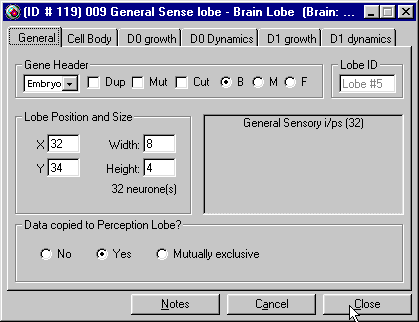
\epsfig {file=img/perception_gensense.png,width=7.39cm}} % 14.78cm
% 	\caption{Interface for Perception Lobe Design -- \textit{copying data} }
% 	\label{fig:perception_gensense}
% \end{figure}
% As can been seen from the above dialog box from the general sense lobe the options for perception are:
% \begin{itemize}
% 	\item No
% 	\item Yes
% 	\item Mutually exclusive
% \end{itemize}~\\
% The brain lobes that are marked as 'Yes' or 'Mutually exclusive' in an original norn are:
% \begin{longtable}{|p{0.25\textwidth}|p{0.15\textwidth}|p{0.65\textwidth}|}
% 	\hline \rowcolor[gray]{0.50} \multicolumn{3}{|c|}{Copied Lobes in Perception} \\
% 	\hline \rowcolor[gray]{0.75} \textbf{Lobe} & \textbf{Size} & \textbf{Data copied to perception lobe?} \\ \hline
% 	\endfirsthead
% 	\hline \rowcolor[gray]{0.50} \multicolumn{3}{|c|}{Copied Lobes in Perception} \\
% 	\hline \rowcolor[gray]{0.75} \textbf{Lobe} & \textbf{Size} & \textbf{Data copied to perception lobe?} \\ \hline
% 	\endhead
% 	\hline 
% 	\endfoot
% 
% 	Drive lobe		&	16 &	Mutually exclusive \\ \hline
% 	Verb lobe		&	16 &	Mutually exclusive \\ \hline
% 	General sense lobe	&	32 &	Yes \\ \hline
% 	Attention lobe 		&	40 &	Yes \\ \hline
% 
% 		\hline
% 	\caption{Copied Lobes in Perception}
% 	\label{tab:Copied_Lobes_in_Perception}\\
% \end{longtable}
% The perception lobe must have a number of cells equal to or greater than the total number of cells in all lobes marked as 'Yes' or 'Mutually exclusive'. The total number of cells in the above lobes equals 104. The size of the perception lobe is 112 so there is a little room to spare there.~\\
% My theory from observation is that starting from the lowest numbered perceptible lobe, the output of each cell of that lobe is copied to the lowest available cell in the perception lobe. So with the perceptible lobes listed above I think the mapping to the perception lobe cells will be:~\\~\\
% \begin{longtable}{|p{0.20\textwidth}|p{0.50\textwidth}|}
% 	\hline \rowcolor[gray]{0.50} \multicolumn{2}{|c|}{Mapping in Perception Lobe Cells} \\
% 	\hline \rowcolor[gray]{0.75} \textbf{Perception cell number} & \textbf{Other lobe cell number} \\ \hline
% 	\endfirsthead
% 	\hline \rowcolor[gray]{0.50} \multicolumn{2}{|c|}{Mapping in Perception Lobe Cells} \\
% 	\hline \rowcolor[gray]{0.75} \textbf{Perception cell number} & \textbf{Other lobe cell number} \\ \hline
% 	\endhead
% 	\hline 
% 	\endfoot
%  	
% 	0--15	&	Drive lobe 0-15 \\ \hline
% 	16--31	&	Verb lobe 0-15 \\ \hline
% 	32--63	&	General sense lobe 0-31 \\ \hline
% 	64--103	&	Attention lobe 0-39 \\ \hline
% 
% 		\hline
% 	\caption{Mapping in Perception Lobe Cells}
% 	\label{tab:Mapping_Perception_Lobe_Cells}\\
% \end{longtable}
% 
% I do not know what the setting 'Mutually exclusive' means. From my tests it appears to do the same as 'Yes' but further experimentation may show otherwise. The following examples will attempt to demonstrate whether my theory about how the perception lobe works and is mapped is correct or not.~\\
% For this example we start with a norn with the normal nine lobes selected in Creatures and we will test the lobes with Perceptible marked as 'Yes'. Run the BrainCellMonitor program, connect to Creatures, and use the 'Add' button to view the following Lobe/Cell/Dendrites:
% \begin{itemize}
% 	\item Lobe 0 Cell 32 Dendrite 0
% 	\item Lobe 0 Cell 63 Dendrite 0
% 	\item Lobe 5 Cell 0 Dendrite 0
% 	\item Lobe 5 Cell 31 Dendrite 0
% \end{itemize}
% 
% \begin{minipage}{0.4\linewidth}
% \begin{figure}[H]
% 	\centerline {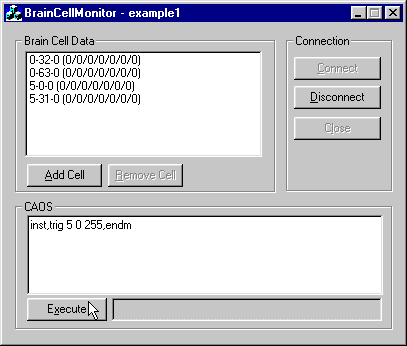
\epsfig {file=img/perception_example1.png,width=5cm}} % 14.36cm
% 	\caption{Interface for Perception Lobe Design -- \textit{how to complete data (1)} }
% 	\label{fig:perception_example1}
% \end{figure}
% \end{minipage}
% \begin{minipage}{0.1\linewidth}\end{minipage}
% \begin{minipage}{0.5\linewidth}
% This will allow us to view the first and last cell in the general sense lobe and compare it against the perceptible cell we think they will be copied to. We will now use CAOS commands to fire particular cells in the general sense lobe (lobe 5) and see if the corresponding cell in the perception lobe (lobe 0) fires with equivalent values.
% \end{minipage}~\\~\\
% 
% Try executing the CAOS command: $inst,trig 5 0 255,endm$. Notice how the perception lobe cell number 32 output number increases and starts to decrease in a similar way to the general sense lobe cell we just fired:
% \begin{figure}[H]
% 	\centerline {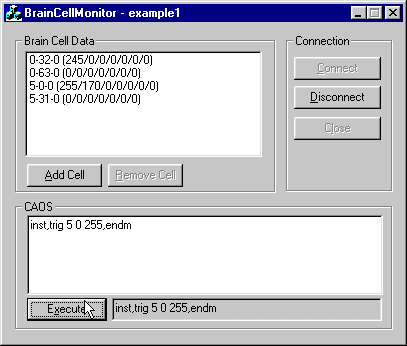
\epsfig {file=img/perception_example2.png,width=7.18cm}} % 14.36cm
% 	\caption{Interface for Perception Lobe Design -- \textit{how to complete data (2)} }
% 	\label{fig:perception_example2}
% \end{figure}
% 
% This seems to imply that our assumed mapping may be correct.~\\
% 
% Try executing the CAOS command: $inst,trig 5 31 255,endm$. Notice how the perception lobe cell number 63output number increases and starts to decrease in a similar way to the general sense lobe cell we just fired. This also seems to confirm our mapping. Try using different cell numbers with lobe 5 and you will see that the mapping we came up with is correct. Now we'll try it with the Attention lobe. Use BrainCellMonitor to view the following cells:
% \begin{itemize}
% 	\item Lobe 0 Cell 64 Dendrite 0
% 	\item Lobe 0 Cell 103 Dendrite 0
% 	\item Lobe 7 Cell 0 Dendrite 0
% 	\item Lobe 7 Cell 39 Dendrite 0
% \end{itemize}
% 
% Try executing the CAOS command: $inst,trig 7 0 255,endm$ and executing the CAOS command: $inst,trig 7 39 255,endm$. Once again you should see the equivalent perception lobes firing.~\\
% 
% You may notice that when doing the General sense example that if you fire both general sense lobes then both perception lobes also fire. But in the Attention example, firing both will only cause one perception lobe cell to fire - why is this? It is because the Attention lobe is marked 'Winner takes all'. This means that only the cell with the highest output actually fires - all the others get automatically set to zero and this data is copied to the perception lobe.~\\
% 
% Well what about the 'Mutually Exclusive' option? Lets try some examples with the Verb lobe which is marked "mutually exclusive". I don't use the Drive lobe just yet as the drives for a norn are constantly changing and can get in the way of our observations. Try viewing the following:
% \begin{itemize}
% 	\item Lobe 0 Cell 16 Dendrite 0
% 	\item Lobe 0 Cell 31 Dendrite 0
% 	\item Lobe 3 Cell 0 Dendrite 0
% 	\item Lobe 3 Cell 15 Dendrite 0
% \end{itemize}~\\
% Try executing the CAOS command: $inst,trig 3 0 255,endm$ and executing the CAOS command: $inst,trig 3 15 255,endm$. Once again you should see the equivalent perception lobes firing. The verb lobe is also marked 'Winner takes all' so you'll see similar effects to that shown in the Attention lobe. You can try examples with the drive lobe as well but as mentioned before the norn drives can get in the way of observation. ~\\
% The Mutually Exclusive option works in the same manner as lobes marked as 'Yes'. The difference between the two options appears when dendrites are linked between the perception lobe and the concept lobe. Usually from 1 to 3 perception cells are linked to a particular concept cell. The perception cells that are linked can change during the lifetime of a norn based on experiences it has encountered. But only one cell from a given Mutually Exclusive lobe can contribute to the forming of a particular concept. Drive is mutually exclusive so we can have a concept of 'hungry' but not 'hungry' and 'tired'. Verb lobe is also mutually exclusive so we can have a concept of being told to 'push' but not being told to 'push' and 'pull'.~\\
% I hope this tutorial/discussion was useful to you in examining the Perception lobe. If you come up with any interesting information I'd love to hear from you. I've updated the BrainActivity program to display the cell details in the perception lobe based on the above observations (as of version 1.3).~\\
% If you've been following this please send feedback to Chris Double (chris@double.co.nz) and let me know what you'd like to see. Thanks!~\\

% \subsection{CDR -- Dendrite Tutorial}
% $<$\textit{http://www.double.co.nz/creatures/tutorial3/tutorial3.htm}$>$~\\
% This tutorial introduces dendrites. It describes what they are and what can be done with them. All the information in this tutorial was discovered using experiments so it may not be completely correct. The information is pretty much a 'brain dump' of what I've encountered while playing around with brain lobes so it may not be organised particularly well. Any corrections, additions or comments are welcome.~\\

\clearpage

\section{Id{\'e}es g{\'e}n{\'e}rales -- <<Discussion>>}

\subsection{D{\'e}finition de r{\^e}gles de bases de conception}

\subsubsection{Quelques indications g{\'e}n{\'e}rales}

% \textbf{<<G{\`e}ne cod{\'e} {\`a} 8 bits : 8 caract{\`e}res (ou autre nombre d{\'e}termin{\'e})>>}~\\
On peut codifier le g{\'e}nome d'un individu <<Agent>> et les informations associ{\'e}es de la fa\c{c}on suivante :
\begin{itemize}
	\item On retient le principe du fichier unique pour chaque agent (identification n{\'e}cessaire). Le g{\'e}nome est d{\'e}crit <<ligne par ligne>>, la liste des variables en t{\^e}te de fichier, et la <<m{\'e}moire>> de l'agent {\`a} la fin (r{\'e}seau de neurones et autres donn{\'e}es).
	\item Un g{\`e}ne est signalis{\'e} par son identification (\textit{header}), et ses param{\`e}tres. Un sch{\'e}ma bien d{\'e}fini est utile pour la lecture du g{\'e}nome (d{\'e}but, en-t{\^e}te, corps, fin) : l'en-t{\^e}te (\textit{header}) concerne notamment l'utilisation de <<drapeaux>> pour indiquer les possibilit{\'e}s de mutation / duplication / d{\'e}l{\'e}tion, et {\'e}galement l'activation du g{\`e}ne, l'{\^a}ge d'int{\'e}r{\^e}t du g{\`e}ne, la liaison au sexe...
	\item Une annotation compl{\'e}mentaire au g{\`e}ne. Cette information est signalis{\'e}e de fa\c{c}on diff{\'e}rente du code du g{\`e}ne. La comparaison genes--exons et annotations--introns peut {\^e}tre interessante. 
	\item Les variables de l'agent peuvent {\^e}tre enregistr{\'e}es de fa\c{c}on similaire, les informations enregistr{\'e}es pour le cerveau de l'agent peuvent {\^e}tre enregistr{\'e}es de cette fa\c{c}on, entrainant une certaine souplesse
	\item Un s{\'e}parateur de un ou plusieurs caract{\`e}res dont l'occurence est nulle ailleurs dans le fichier : fin de ligne, tabulation...
	\item La lecture du g{\'e}nome est effectu{\'e}e au d{\'e}but de la simulation (chargement en m{\'e}moire) pour permettre une execution it{\'e}rative. 
\end{itemize}~\\

L'utilit{\'e} du s{\'e}parateur est d'{\'e}viter le chevauchement des informations ou un mauvais fonctionnement du programme. En effet, l'ouverture de fichiers <<gen>> de \textit{Creatures} montre que la structure g{\'e}n{\'e}tique des norns est {\'e}tablie selon ce sch{\'e}ma : une succession de \emph{genexxxxxxxxgend} contigu{\" e}s. Ceci est une reprise et inspiration directe du syst{\`e}me utilis{\'e} dans \textit{Creatures}. Ce syst{\`e}me semble efficace mais peut entra{\^\i}ner un programme long {\`a} executer lors la lecture du fichier et le chargement d'un individu.~\\

Une id{\'e}e est d'attribuer {\`a} chaque g{\`e}ne une fonction pr{\'e}cise, et de permettre un codage qui peut {\^e}tre affect{\'e} par des changements. Chaque individu est enregistr{\'e} avec l'ensemble de son information g{\'e}n{\'e}tique (IG) : le <<d{\'e}codage>> du g{\`e}ne permet son chargement en m{\'e}moire.  Un ensemble de variables est disponible, notamment lors de l'<<execution>> des g{\`e}nes (sous forme de m{\'e}thodes informatiques). Un m{\'e}canisme pour les mutations, duplications et d{\'e}l{\'e}tions est {\`a} pr{\'e}voir.~\\

% \rule{10cm}{0.5mm}~\\

\subsubsection{Encodage de l'Information G{\'e}n{\'e}tique}

% \emph{Code des triplets des caract{\`e}res de code de l'ADN / ARN}~\\
\begin{table}[ht]
	\begin{center}
		\begin{tabular}{|c c c c c c c c c c c c c c c c|}
		\hline
			aaa&aag&aat&aac&gaa&gag&gat&gac&taa&tag&tat&tac&caa&cag&cat&cac\\
			aga&agg&agt&agc&gga&ggg&ggt&ggc&tga&tgg&tgt&tgc&cga&cgg&cgt&cgc\\
			ata&atg&att&atc&gta&gtg&gtt&gtc&tta&ttg&ttt&ttc&cta&ctg&ctt&ctc\\
			aca&acg&act&acc&gca&gcg&gct&gtc&tca&tcg&tct&tcc&cca&ccg&cct&ccc\\
		\hline
		\end{tabular}
	\end{center}
	\caption{Tableau des 64 triplets standards du code g{\'e}n{\'e}tique}
	\label{tab:InformationGenetiqueStandardTriplets}
\end{table}

Il est n{\'e}cessaire d'{\'e}tablir comme constituant du <<g{\'e}nome>> de l'agent un code avec plusieurs caract{\`e}res, pour l'enregistrement en dehors du programme ou pour tout travail sur les g{\`e}nes ou les g{\'e}nomes entiers (comparaison, croisement, mutation, duplication, d{\'e}l{\'e}tion, {\'e}changes...).  L'id{\'e}e de base dans ce cadre est l'utilisation du symbole {\`a} une lettre des acides amin{\'e}s) : leur nombre d{\'e}pend du nombre de commandes distinctes utilisables dans un g{\`e}ne, une m{\^e}me information pouvant {\^e}tre utilis{\'e}e plusieurs fois. Il faut d{\'e}terminer les informations possibles et leur code d'appel (passage du <<triplet de nucl{\'e}otides>> {\`a} l'<<Acide Amin{\'e}>>), selon les crit{\`e}res de s{\'e}lection : information la plus simple et la plus g{\'e}n{\'e}rale possible, une information unitaire pouvant {\^e}tre facilement utilisable.~\\

Plusieurs {\'e}tapes de construction du code de l'Information G{\'e}n{\'e}tique (IG), associ{\'e} {\`a} une utilisation du dogme central de la biologie (transcription puis traduction $ADN \rightarrow ARN \rightarrow AA$) : 
\begin{enumerate}
	\item Coder g{\`e}ne par g{\`e}nes suivant le mod{\`e}le de \emph{Creatures} : 
	\begin{itemize}
		\item D{\'e}terminer le code ou la fonction g{\'e}n{\'e}rique pour chaque type de g{\`e}ne. 
		\item Codage des g{\`e}nes avec indication du type de g{\`e}ne et des param{\`e}tres n{\'e}cessaires. 
		\item {\'E}tablir un fichier g{\'e}n{\'e}tique exemple avec un g{\`e}ne par ligne. 
		\item Tester le mod{\`e}le
	\end{itemize}
	\item Passer en code <<ADN / ARN / AA>> en conservant un g{\`e}ne par ligne (directement codant), un <<Acide Amin{\'e}>> correspond {\`a} un caract{\`e}re unique {\`a} transcrire dans l'ordre.  
	\item Conserver le code de l'{\'e}tape pr{\'e}c{\'e}dente (toujours un g{\`e}ne par ligne) en ajoutant un syst{\`e}me de promoteur et des signaux de fin de g{\`e}ne. 
	\item \textit{Ins{\'e}rer des introns (parties non codantes, annotations) avec de des signaux <<d'{\'e}pissage>> (pr{\'e}voir {\'e}ventuellement l'{\'e}pissage alternatif). }
	\item Regrouper les g{\`e}nes en <<chromosomes>> (un par ligne) et tester avec du code sans signification entre g{\`e}nes (id{\'e}alement proche des <<introns>>). 
	\item \textit{<<Petits ARN>> et interf{\'e}rence : cr{\'e}er des g{\`e}nes qui interviennent au niveau de la traduction ou de l'activit{\'e} des g{\`e}nes. }
\end{enumerate}~\\

% \rule{10cm}{0.5mm}~\\

\textbf{Construction avec les bases ``a,c,t,g''} (ou autres lettres comme ``u,b,v,p'')~\\
Il faut d{\'e}terminer les g{\`e}nes de base n{\'e}cessaires pour un <<organisme exp{\'e}rimental>> : m{\'e}tabolisme, nutrition, croissance, reproduction... et utilisation des 64 combinaisons pour les triplets, il est possible d'utiliser des quadruplets (256 combinaisons).~\\

\textbf{Protocole de fabrication de cette fonctionnalit{\'e} de codage en bases}
\begin{enumerate}
	\item {\'E}tablir un algorithme pour chaque type g{\`e}ne de mani{\`e}re {\`a} ce qu'il soit le plus simple possible mais aussi optimal (nombre de variables, nombre de commandes, rapidit{\'e} d'ex{\'e}cution...). 
	\item Obtenir des informations unitaires : caract{\`e}re, lettre ou chiffre. 
	\item Transcrire cette information dans un code en triplet ou quadruplet. 
	\item Observer les r{\'e}sultats {\`a} l'utilisation : g{\`e}ne par g{\`e}ne, fonctionnement d'un organisme, cons{\'e}quences des mutations. % (s{\'e}lection <<naturelle>>, blocage du programme)...
	\item {\'E}ventuellement : am{\'e}liorer les algorithmes, cr{\'e}er de nouveaux g{\`e}nes ou en combiner pour obtenir un comportement global. 
\end{enumerate}~\\

% \rule{10cm}{0.5mm}~\\
% \textbf{Programmation des routines g{\'e}n{\'e}tiques}~\\
Les param{\`e}tres n{\'e}cessaires pour les g{\`e}nes sont relativement r{\'e}duits : on peut se contenter d'informations num{\'e}riques, mais il faut {\'e}galement pouvoir enregistrer les donn{\'e}es d'annotation. Les chiffres de 0 {\`a} 9 avec des caract{\`e}res de d{\'e}but et de fin de g{\`e}ne sont suffisants (12 caract{\`e}res) mais il faut {\'e}galement pr{\'e}voir des caract{\`e}res alphab{\'e}tiques (26 caract{\`e}res, plus des caract{\`e}res permettant de s{\'e}parer les annotations du reste, quitte {\`a} utiliser leur r{\'e}p{\'e}tition.~\\

Ces caract{\`e}res {\'e}tant utilisables {\'e}galement pour enregistrer la m{\'e}moire des individus ainsi programm{\'e}s, aucun autre jeu de caract{\`e}res n'est n{\'e}cessaire {\`a} ce stade. En utilisant une certaine redondance dans le code on peut ainsi compl{\'e}ter et arriver {\`a} une biblioth{\`e}que de 64 caract{\`e}res utilisant des triplets, un tel <<g{\'e}nome>> est facilement lisible par un automate utilisant une table de hashage (structure en arbre de lecture), la longueur du g{\'e}nome importe peu, sauf pour la longueur du chargement en m{\'e}moire.~\\

Il est n{\'e}cessaire de cr{\'e}er des \emph{programmes de tests ind{\'e}pendants} pour la mise en place et le test des g{\`e}nes (cerveau/lobes avec entr{\'e}es et sorties ; recepteurs/drivers/emetteurs avec affichage r{\'e}gulier des variables ; ...). Les individus de d{\'e}part sont pr{\'e}-{\'e}tablis pour des tests (et {\'e}ventuellement pour la suite). ~\\

\clearpage

\textbf{Enregistrement des individus}
\begin{itemize}
	\item Enregistrement sp{\'e}cifique au logiciel (sauvegarde en cours). 
	\item {\`A} la demande pendant le d{\'e}roulement de l'application (export)
	\item Sauvegarde ext{\'e}rieures avec utilisation du format GenBank ?? EMBL ?? FASTA ?? 
\end{itemize}~\\

\begin{table}[H]
\fbox{%
\begin{minipage}{0.9\textwidth}

\begin{enumerate}
	\item \scriptsize{\texttt{\underline{Bact{\'e}ries avec un chromosome comportant 4 groupes de g{\`e}nes principaux}}}
	\begin{enumerate}
		\item \scriptsize{\texttt{Nutrition (recherche d'{\'e}nergie : crit{\`e}res nutritifs des {\'e}l{\'e}ments fix{\'e}s au d{\'e}part)}}
		\item \scriptsize{\texttt{Assimilation (transformer l'{\'e}nergie en vue d'une utilisation ou d'un stockage {\'e}ventuel)}}
		\item \scriptsize{\texttt{Croissance (d{\'e}veloppement, mouvement...)}}
		\item \scriptsize{\texttt{Reproduction (et mutations vari{\'e}es plus ou moins rares, croisements si reproduction sexu{\'e}e ou {\'e}changes de g{\`e}nes : ponts cellulaires et virus)}}
	\end{enumerate}
	\item \scriptsize{\texttt{Mort par sureffectifs, disparition des moins adapt{\'e}s...}}
	\item \scriptsize{\texttt{Mutation est substitution, deletion ou addition d'une base (si codage en bases).}}
	\item \scriptsize{\texttt{Lecture de l'ADN : de M (m{\'e}thionine) {\`a} $\ast$ (stop) ou une suite de caract{\`e}res identiques.}}
\end{enumerate}

\end{minipage}%
}
\caption{Exp{\'e}rimentation de base avec une bact{\'e}rie de test. }
\label{fig:BacteriaExperiment}
\end{table}

Rien ne doit {\^e}tre modifi{\'e} dans le programme au cours de son execution par un utilisateur : toute demande sauvegarde se fait en externe ({\`a} moins d'une fonctionnalit{\'e} pr{\'e}cise de r{\'e}-initialisation), il est utile dans ce cadre de disposer d'un outil d'import / export dans la simulation.~\\

Un tel outil (int{\'e}gr{\'e} ou non au logiciel) peut permettre l'analyse et la manipulation des g{\'e}nomes des individus (agents, organismes) int{\'e}gr{\'e}s au mod{\`e}le. De plus, l'id{\'e}e est de pouvoir cr{\'e}er de nouveaux individus avec un outil facile {\`a} manipuler et permettant des croisements ou une observation directe des individus. 

\subsubsection{Utilisation du <<multithreading>>}

Ceci est pr{\'e}vu pour la fin mais ne doit pas {\^e}tre oubli{\'e} lors du d{\'e}veloppement du logiciel ; le choix a port{\'e} sur une mod{\'e}lisation synchrone plut{\^o}t que asynchrone, associ{\'e} {\`a} une gestion de la priorit{\'e} des processus (\textit{Thread}).
\begin{itemize}
	\item all{\'e}ger le programme avec un cycle d'execution it{\'e}rable, 
	\item utilisation de fonctions ind{\'e}pendantes avec conservation et modification en m{\'e}moire vive.
\end{itemize}

\subsection{Id{\'e}es d'int{\'e}gration dans le mod{\`e}le}

\subsubsection{Agents infectieux : bact{\'e}ries, virus et plasmides}

Le principe est ici de d{\'e}finir des parasites pouvant s'auto-r{\'e}pliquer et s'auto-modifier dans un organisme / individu / agent h{\^o}te et entrainant {\'e}ventuellement des perturbations dans celui-ci. Un tel parasite entra{\^\i}ne la production d'Antig{\`e}nes (Ag) n{\'e}cessaires pour les production de synth{\`e}ses bact{\'e}riennes ou virales ; ceci est contr{\'e} par des Anticorps (Ac) de l'h{\^o}te. Il y a insertion d'un code parasite dans le g{\'e}nome h{\^o}te, ce qui entra{\^\i}ne une biochimie particuli{\`e}re, voire des comportements particuliers (production de particules virales par exemple).~\\

\textbf{Propri{\'e}t{\'e}s des plasmides bact{\'e}riens}~\\
\begin{tabular}{|p{8cm}|p{8cm}|}
\hline
 R{\'e}plication autonome (dans l'h{\^o}te).			& Incompatibilit{\'e} des plasmides apparent{\'e}s. 		\\
 Fertilit{\'e} (autotransfert d'un h{\^o}te {\`a} l'autre).	& Mobilisation (utilise h{\^o}te pour transmission).		\\
 Modification (g{\`e}nes en + ou en -).				& Production de toxines. 					\\
 Fusion des r{\'e}plicons.					& R{\'e}sistance/sensibilit{\'e} ({\`a} certains facteurs). 	\\
 Mutag{\`e}ne/antimutag{\`e}ne.					& Caract{\`e}res m{\'e}taboliques. 				\\
 Facteurs adh{\'e}rence/pathog{\'e}nicit{\'e}. 			& Recombinaison/transposition des g{\`e}nes.		 	\\
 Capacit{\'e} d'induction de tumeurs.				& 								\\
 \hline
\end{tabular}~\\

\clearpage

Ces {\'e}l{\'e}ments g{\'e}n{\'e}tiques ne font strictement pas partie du g{\'e}nome de l'agent (un chromosome <<{\`a} part>> suppl{\'e}mentaire) mais peuvent {\'e}ventuellement y {\^e}tre int{\'e}gr{\'e}s de fa\c{c}on d{\'e}finitive (dans la mod{\'e}lisation) comme des g{\`e}nes d'agents infectieux (bact{\'e}ries, virus ou plasmides). 
\begin{itemize}
	\item Informations pour le tranfert avec plus ou moins d'autres g{\`e}nes. 
	\item Transmission du donneur (\textit{F+}) au receveur (\textit{F-}), ce dernier ne poss{\'e}dant pas le <<plasmide>>, qui peut {\^e}tre perdu ou {\'e}limin{\'e}. 
	\item Transmit aussi lors de la scissiparit{\'e} des individus (reproduction asexu{\'e}e). 
	\item Influence sur la s{\'e}lection des individus (caract{\`e}res m{\'e}taboliques, sensibilit{\'e} / r{\'e}sistance). 
	\item \textit{HFr} = comme les \textit{F+}, mais au lieu du simple plasmide, c'est l'information g{\'e}n{\'e}tique compl{\`e}te qui est copi{\'e}e chez le receveur (copie totale ou fragmentaire, le receveur ne devient pas forc{\'e}ment donneur). 
\end{itemize}

\subsubsection{Syst{\`e}me immunitaire}

Le syst{\`e}me immunitaire chez les organismes {\'e}volu{\'e}s utilise le syst{\`e}me des Anticorps (Ac) compos{\'e}s de parties fixes de  parties variables (code de reconnaissance sp{\'e}cifiques) ; sp{\'e}cifit{\'e} de r{\'e}action avec des Antig{\`e}nes (Ag) d'origine ext{\'e}rieure. Le Syst{\`e}me Immunitaire (SI) est un programme de reconnaissance g{\'e}n{\'e}ral qui agit si un Ag n'est pas dans la base de l'individu, est inconnu, ou reconnu comme <<{\'e}tranger>> (d{\'e}j{\`a} rencontr{\'e} auparavant).~\\

De fa\c{c}on g{\'e}n{\'e}rale dans le mod{\`e}le cr{\'e}{\'e} ici, il s'agit plus simplement d'utiliser certaines variables comme n{\'e}cessaires au d{\'e}veloppement des agents infectieux et d{\'e}clencheurs des comportements infectieux (Antig{\`e}nes qui provoquent la production de nouveaux objets comme des particules virales). Pour contrer ces r{\'e}actions, l'organisme h{\^o}te poss{\`e}de des r{\'e}actions biochimiques (associ{\'e}es {\`a} des variables Anticorps) qui font diminuer la quantit{\'e} d'antig{\`e}nes pr{\'e}sents afin d'{\'e}viter les r{\'e}actions li{\'e}es au m{\'e}tabolisme import{\'e} par le parasite. 

\subsubsection{{\'E}tude {\'e}volutive}

L'id{\'e}e est d'effectuer une {\'e}tude {\'e}volutive au sein d'une telle simulation et de travailler {\`a} partir d'une taxonomie (classification selon Phylum, Classe, Ordre, Famille, Genre, Esp{\`e}ce, Vari{\'e}t{\'e}). L'{\'e}tude s'effectuant au d{\'e}part par phylum et par esp{\`e}ces directement mod{\'e}lis{\'e}es. Une d{\'e}finition des phylum de d{\'e}part est la suivante :~\\
\begin{minipage}{8cm}
\begin{itemize}
	\item \emph{Silicobacter} : <<bact{\'e}ries>>
	\item \emph{Silicoviridae} : <<virus>>
	\item \emph{Silicoviriditae} : <<plantes>>
	\item \emph{Silicoanimae} : <<animaux>>
\end{itemize}
\end{minipage}\hfill\begin{minipage}{10cm}
Un cinqui{\`e}me phylum \emph{Silicodaemon} est pr{\'e}vu pour d{\'e}finir les agents programm{\'e}s dans l'environnement mais non susceptible d'{\'e}volution, pour assurer un renouvellement de l'environnement. L'objectif est de d{\'e}finir des esp{\`e}ces de d{\'e}part dans les cinq phylum et {\'e}tudier l'{\'e}volution obtenue. 
\end{minipage}~\\

Les outils classiques de comparaison de s{\'e}quence seront ensuite utilis{\'e}s pour classer les esp{\`e}ces et s{\'e}quences obtenues suite {\`a} l'{\'e}volution (dot-plot, algorithmes SW et NW, phylog{\'e}nie, FASTA, BLAST...). 

\subsubsection{G{\`e}nes particuliers}

Une id{\'e}e concerne l'utilisation de g{\`e}nes <<sp{\'e}ciaux>> utilisant les d{\'e}finition pr{\'e}-{\'e}tablies mais amenant des comportements particuliers et ayant un impact au niveau {\'e}volutif (autres que ceux des agents infectieux). Quelques id{\'e}es glan{\'e}es ici~\cite{BearDarwin01,BearDarwin03} et l{\`a}~\cite{DiasporaKubeMc} {\`a} propos de g{\`e}nes th{\'e}oriques connus pour leur <<performance>>, enregistr{\'e}s, encod{\'e}s dans les g{\'e}nomes et plus ou moins activ{\'e}s (selon stress ou autre activit{\'e} particuli{\`e}re). Il peut s'agir de g{\`e}nes naturellement pr{\'e}sent dans les g{\'e}nomes ou de g{\`e}nes viraux plus ou moins actifs provoquant des comportements particuliers ou des remaniements de g{\'e}nome. 
\begin{itemize}
	\item Des \textbf{{\'e}l{\'e}ments transposables}~\cite{LeRiBi03,RiBiGo02,RiMaGo02} : transposons, r{\'e}trotransposons et {\'e}l{\'e}ments viraux analogues... Ces {\'e}l{\'e}ments peuvent amener {\`a} un remaniement du g{\'e}nome <<h{\^o}te>>.
	\item \textbf{\emph{Req Queen} (RQ)} : engendre des ph{\'e}nom{\`e}nes de Mutation / Duplication / D{\'e}l{\'e}tion des g{\`e}nes lors de la vie d'un individu et non plus seulement lors de la reproduction, remanie l'ordre des g{\`e}nes, voire provoque la fusion entre deux individus de la m{\^e}me esp{\`e}ces ou d'esp{\`e}ces diff{\'e}rentes. 
	\item \textbf{Chi (A/B/C)}~\cite{DiasporaKubeMc} : marqueur d'une capacit{\'e} particuli{\`e}re, qui provoque un comportement inn{\'e} (r{\'e}seau de neurone ou lobe fig{\'e}). 
	\item \textbf{SHEVA}~\cite{BearDarwin01,BearDarwin03} : comme les g{\`e}nes RQ mais SHEVA provoque l'apparition d'un virus qui am{\`e}ne le ph{\'e}nom{\`e}ne {\`a} s'exprimer chez d'autres individus, via une transmission virale et / ou des ph{\'e}romones. 
\end{itemize}

\clearpage

\subsubsection{Reproduction asexu{\'e}, sexu{\'e}e...}

On peut distinguer deux grands modes de reproduction, sexu{\'e}e et asexu{\'e}e. L'id{\'e}e est de reprendre le principe biologique de reproduction : le cycle de vie cellulaire (pour la reproduction asexu{\'e}e) et de pr{\'e}paration hormonale (seuil de fertilit{\'e}, cycle de fertilit{\'e}).
\begin{itemize}
	\item \underline{Reproduction asexu{\'e}e}~\\
		Copie du g{\'e}nome et apparition d'un organisme identiques (<<scissiparit{\'e}>>) {\`a} quelques modifications pr{\`e}s (mutation, duplication, d{\'e}l{\'e}tion) avec remise {\`a} z{\'e}ro du niveau hormonal si il y a utilisation d'un cycle hormonal (une ou plusieurs hormones). 
	\item \underline{Reproduction sexu{\'e}e}~\\
		Au moins deux sexes, \emph{parth{\'e}nog{\'e}n{\`e}se possible}, \textbf{fabrication de gam{\`e}tes lors de l'atteinte de seuil(s) hormonaux (stimulus)} : 
		\begin{itemize}
			\item \textbf{\textit{m{\^a}le}} avec seuil hormonal d{\'e}clenchant la fertilit{\'e} (<<testot{\'e}rone>>).
			\item \textbf{\textit{femelle}}, cycle hormonal (<<\oe strog{\`e}ne>>, <<progest{\'e}rone>>...). 
			\item autres sexes, plut{\^o}t hypoth{\`e}se d'un syst{\`e}me de cycle. 
		\end{itemize}
		Si il y a contact de gam{\`a}tes ou lors de phases communes de fertilit{\'e}, ceci provoque la r{\'e}alisation du croisement entre les gam{\`e}tes de diff{\'e}rents individus de sexes diff{\'e}rents et un changement de production des hormones cycliques (pour l'individu porteur / producteur de l'\oe uf. \emph{Si le nombre de g{\`e}nes ou la taille du g{\'e}nome est significativement diff{\'e}rent(e), plusieurs possibilit{\'e}s sont admises : }
		\begin{itemize}
			\item arr{\^e}t car esp{\`e}ces diff{\'e}rentes (on consid{\`e}re une esp{\`e}ce poss{\`e}de un nombre de g{\`e}nes d{\'e}finit avec une tol{\'e}rance) ; 
			\item fusion des gam{\`e}tes (et cr{\'e}ation d'une <<nouvelle esp{\`e}ce>>). 
		\end{itemize}
		Le croisement des g{\'e}nomes des parents s'effectue via l'association des gam{\`e}tes cr{\'e}{\'e}s (choix al{\'e}atoire des g{\`e}nes, crossing-over si polyplo{\"\i}die) quelques modifications peuvent intervenir (mutation, duplication, d{\'e}l{\'e}tion).
	\item Les particularit{\'e}s du nouvel individu sont li{\'e}es {\`a} son patrimoine g{\'e}n{\'e}tique, {\`a} ce niveau, il y a n{\'e}cessit{\'e} de cr{\'e}er un \textbf{identifiant unique} qui peut {\^e}tre cod{\'e} g{\'e}n{\'e}tiquement...
\end{itemize}~\\

Un questionnement {\`a} ce niveau est la conception d'esp{\`e}ces \textbf{ovipares ou vivipares}, notamment pour les esp{\`e}ces sexu{\'e}es. Il est s{\^u}rement plus simple de <<provoquer>> la cr{\'e}ation d'un \oe uf et de permettre son {\'e}volution en individu {\`a} diff{\'e}rents stades (\oe uf, embryon / larve...) ; il suffit de pr{\'e}voir pr{\'e}voir un emplacement de stockage des gam{\`e}tes dans les individus (tous sexes confondus) et {\'e}ventuellement pour le croisement des gam{\`e}tes.~\\

Une autre questionnement concerne la plo{\"i}die des organismes mod{\'e}lis{\'e}s, au d{\'e}part mod{\'e}liser des organismes haplo{\"i}des posera moins de probl{\`e}mes pour la reproduction tant asexu{\'e}e que sexu{\'e}e (copie du g{\'e}nome, crossing-over).  La complexit{\'e} de l'utilisation de la polyplo{\"i}die intervient dans la reproduction sexu{\'e}e (n{\'e}cessit{\'e} des gam{\`e}tes), la parth{\'e}nog{\'e}n{\`e}se peut {\^e}tre utile {\`a} ce stade pour tester une reproduction sans croisement.~\\

Le \textbf{but des modifications telles que mutations / duplications / d{\'e}l{\'e}tions} est d'{\'e}viter l'uniformisation de l'Information G{\'e}n{\'e}tique (IG) et s'effectue sur chacun des g{\`a}nes (ou sur l'ensemble du g{\'e}nome avec des indels). Il se pose {\'e}galement la question de l'activation / inactivation des g{\`e}nes dans le g{\'e}nome d'un individu d'o{\`u} l'int{\'e}r{\^e}t de l'en-t{\^e}te dans l'encodage des g{\`e}nes.~\\

% \rule{10cm}{0.5mm}~\\
% \clearpage

\subsubsection{Parth{\'e}nog{\'e}n{\`e}se -- \emph{Extraits de Wikipedia}~\cite{WikiPathenoGenese}}

La parth{\'e}nogen{\`e}se (ou parth{\'e}nog{\'e}n{\`e}se) est la multiplication {\`a} partir d'un gam{\`e}te femelle non f{\'e}cond{\'e}. Ce ph{\'e}nom{\`e}ne s'observe naturellement chez certaines esp{\`e}ces v{\'e}g{\'e}tales et animales, mais peut {\'e}galement {\^e}tre provoqu{\'e} artificiellement. La parth{\'e}nogen{\`e}se est une reproduction monoparentale. Cette reproduction a un avantage s{\'e}lectif car elle produit un grand nombre d'individus sans la pr{\'e}sence de l'organisme m{\^a}le. Ce ph{\'e}nom{\`e}ne donne :
\begin{itemize}
	\item parth{\'e}nogen{\`e}se th{\'e}lytoque : uniquement des femelles,
	\item parth{\'e}nogen{\`e}se arrh{\'e}notoque : uniquement des m{\^a}les,
	\item parth{\'e}nogen{\`e}se deut{\'e}rotoque / amphot{\'e}rotoque : m{\^a}les et femelles.
\end{itemize}
\clearpage

Selon les hypoth{\`e}ses actuelles la multiplication asexu{\'e}e peut avoir des avantages {\`a} court terme quand la croissance d{\'e}mographique est rapide ou quand l'environnement est stable. Au contraire la reproduction offre {\`a} long terme un net avantage en permettant une adaptation plus rapide {\`a} des environnements changeants. Les lign{\'e}es se reproduisant par multiplication asexu{\'e}e peuvent accro{\^\i}tre leur nombre rapidement parce que, comme les individus sont toujours femelles, chacun peut produire des \oe ufs qui {\'e}cloront. Dans les populations s{\'e}par{\'e}es en sexes certains individus sont m{\^a}les et ne peuvent donc pas avoir de prog{\'e}niture. Autant dire que dans des conditions id{\'e}ales une lign{\'e}e asexu{\'e}e aura en gros un taux de croissance d{\'e}mographique double par rapport {\`a} une population compos{\'e}e pour moiti{\'e} de m{\^a}les, c'est ce qu'on appelle le d{\'e}savantage reproductif et plus couramment le <<two-fold cost of sex>>. Les organismes qui peuvent se reproduire par parth{\'e}nogen{\`e}se sont aussi plus capables de coloniser des habitats isol{\'e}s comme les {\^\i}les oc{\'e}aniques, puisqu'il suffit qu'un seul exemplaire de l'esp{\`e}ce (n{\'e}cessairement femelle) atteigne l'habitat pour commencer {\`a} le peupler.~\\

Une autre cons{\'e}quence de la reproduction asexu{\'e}e, qui peut avoir autant d'avantages que d'inconv{\'e}nients, c'est que la prog{\'e}niture est g{\'e}n{\'e}tiquement identique ou presque identique {\`a} son parent (sauf en cas de mutation). Cette similarit{\'e} g{\'e}n{\'e}tique peut {\^e}tre favorable si le g{\'e}notype convient exactement {\`a} un environnement stable, mais elle est d{\'e}savantageuse si l'environnement change. Par exemple, s'il appara{\^\i}t un nouveau pr{\'e}dateur, un nouvel environnement, ou un nouvel agent pathog{\`e}ne auquel un individu est mal adapt{\'e}, sa lign{\'e}e parth{\'e}nog{\'e}n{\'e}tique sera tout aussi vuln{\'e}rable que lui. Par contre, une lign{\'e}e produite par reproduction sexu{\'e}e a de meilleures possibilit{\'e}s d'adaptation gr{\^a}ce {\`a} la recombinaison g{\'e}n{\'e}tique par laquelle chaque individu pr{\'e}sente un g{\'e}notype original.

% \rule{10cm}{0.5mm}~\\
% \clearpage

\subsubsection{Biochimie et voies m{\'e}taboliques}

Une id{\'e}e majeure de la construction de ce syst{\`e}me de mod{\'e}lisation est d'int{\'e}grer un syst{\`e}me biochimique aux organismes mod{\'e}lis{\'e}s, avec un ensemble de donn{\'e}es sur la chimie des agents, ainsi que des g{\`e}nes codant l'utilisation de ces {\'e}l{\'e}ments chimiques. L'ensemble des {\'e}l{\'e}ments chimiques utilis{\'e}s dans le mod{\`e}le sont simplement rassembl{\'e}s dans une m{\^e}me table, avec un ensemble de r{\^e}gles d'utilisation.~\\

De fa\c{c}on compl{\'e}mentaire aux {\'e}l{\'e}ments simples (liste issue de la table de Mendele{\"i}ev), ce tableau est pr{\'e}vu pour comprendre {\'e}galement les compos{\'e}s chimiques (mol{\'e}cules, compos{\'e}s de mol{\'e}cules...) ainsi que diff{\'e}rents <<drapeaux>> utiles pour mod{\'e}liser un organisme. L'objectif est de reprendre le mod{\`e}le connu de diff{\'e}rentes voies m{\'e}taboliques des organismes procaryotes et eucaryotes, dans leurs diff{\'e}rentes {\'e}tapes : glycolyse, b{\'e}ta-oxydation des acides gras (h{\'e}lice de Lynen), cycle de lacide citrique (Cycle de Krebs)... Chaque enzyme impliqu{\'e}e (catalysant une r{\'e}action chimique) {\'e}tant reprise dans un mod{\`e}le biochimique encod{\'e} g{\'e}n{\'e}tiquement dans le mod{\`e}le, dans chacun des organismes.~\\

\begin{minipage}[c]{10cm}
\textbf{M{\'e}tabolisme des sucres -- \emph{Glycolyse}}. 
\begin{enumerate}
	\item Activation des hexoses (phosphatation du glucose). 
	\item Isom{\'e}risation (Fructore 1,6 phosphate). 
	\item Trioses hosphates. 
	\item R{\'e}cup{\'e}ration de l'{\'e}nergie (glycerate, pyruvate...). 
\end{enumerate}~\\
\textbf{M{\'e}tabolisme des acides gras~\\ \emph{H{\'e}lice de Lynen}}
\begin{enumerate}
	\item Activation de l'Acide Gras (Acyl-CoA {\`a} \emph{n} carbones). 
	\item D{\'e}shydrog{\'e}nation Acyl-CoA. 
	\item Hydratation double liaison. 
	\item D{\'e}shydrog{\'e}nation. 
	\item Coupure (ac{\'e}tylCoA + AcylCoA {\`a} \emph{n-2} carbones). 
	\item Retour autant que n{\'e}cessaire au deuxi{\`e}me point. 
\end{enumerate}
\end{minipage}\hfill
\begin{minipage}[c]{8cm}
\textbf{M{\'e}tabolisme {\'e}nerg{\'e}tique~\\ \emph{Cycle de Krebs}}
\begin{enumerate}
	\item 
	\item 
	\item 
	\item 
	\item 
	\item 
	\item 
	\item 
	\item 
\end{enumerate}~\\~\\~\\
\end{minipage}

\clearpage

\begin{figure}[H]
	\centerline {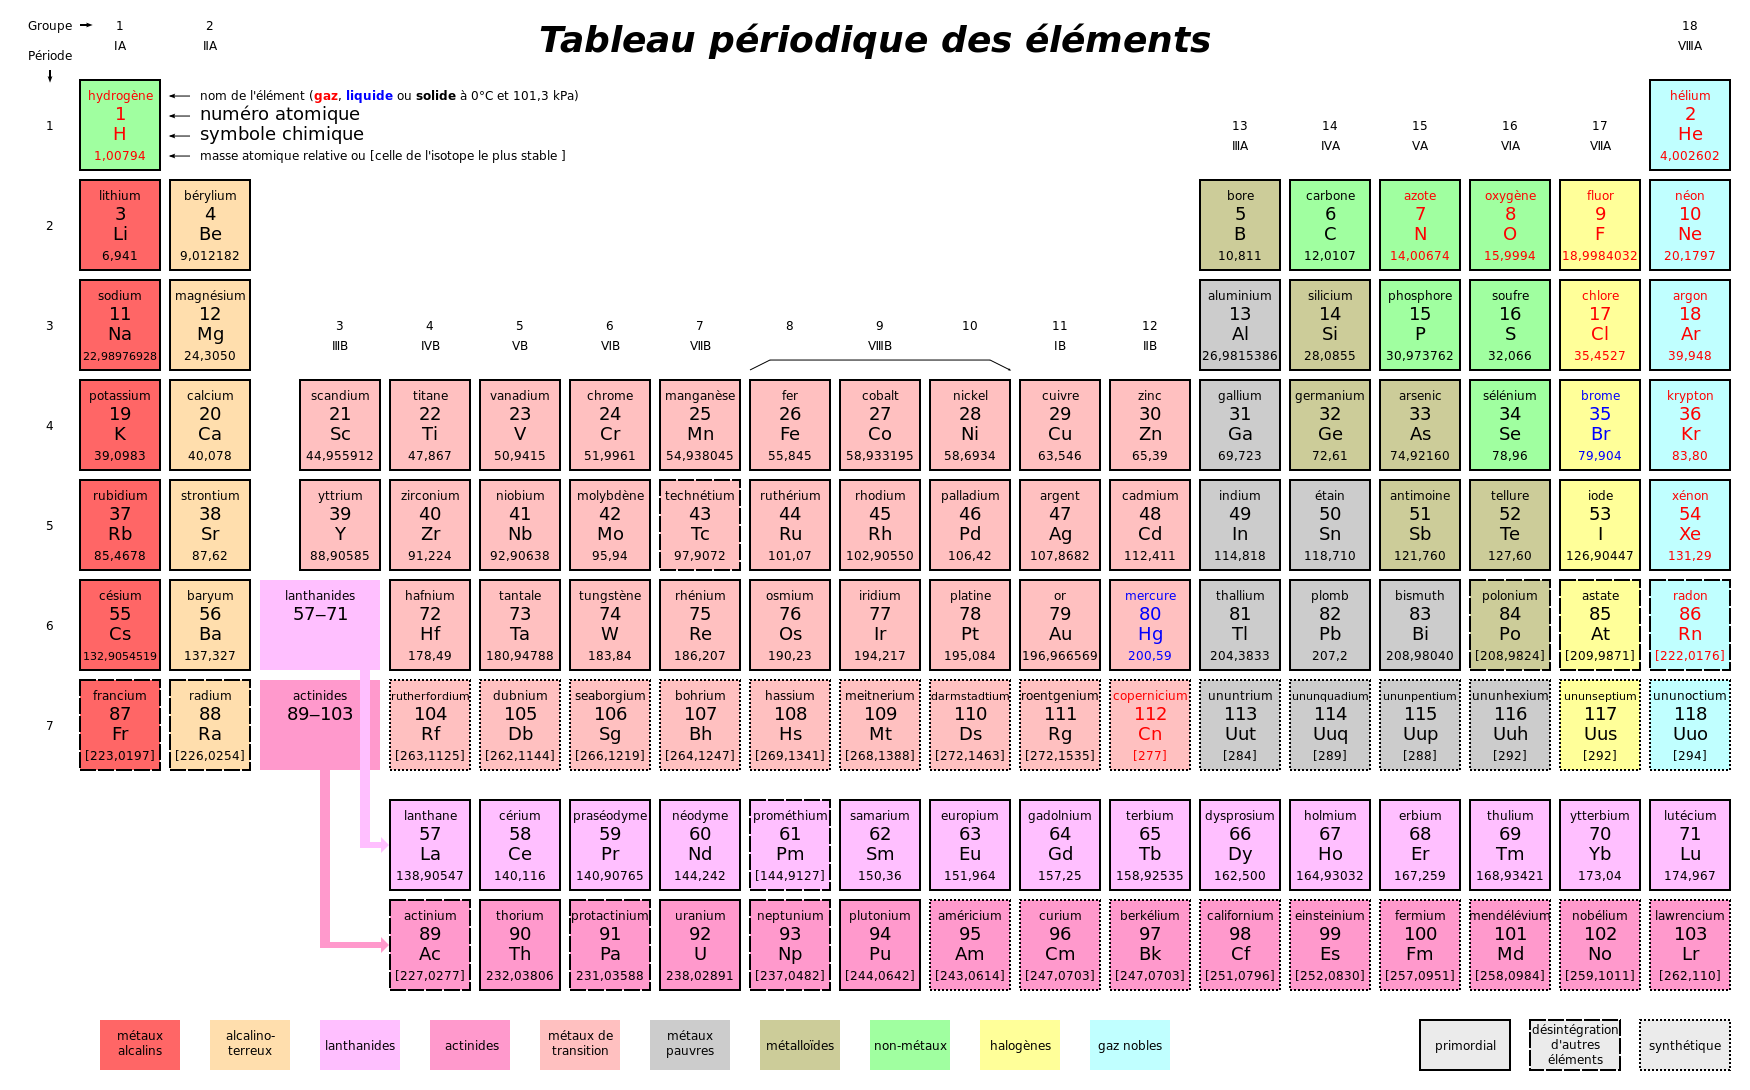
\epsfig {file=img/mendeleievTable.png,width=18cm}}
	\caption{Tableau de Mendele{\"i}ev. }
	\label{fig:mendeleievTable}
\end{figure}

\begin{figure}[H]
	\centerline {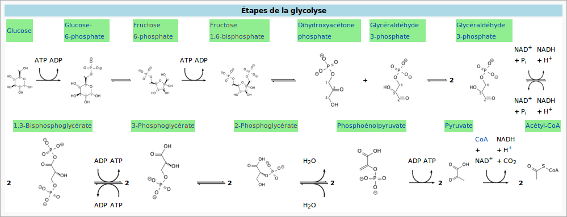
\epsfig {file=img/glycolyse.png,width=18cm}}
	\caption{{\'E}tapes de la glycolyse. }
	\label{fig:glycolyse}
\end{figure}

% \begin{table}[h]
% 	\centering
% \rowcolors{2}{verylightgrey}{white}
\begin{longtable}{|p{0.10\textwidth}|p{0.20\textwidth}|c|p{0.20\textwidth}|p{0.20\textwidth}|c|p{0.20\textwidth}|}
\hline
	\rowcolor{verylightgrey} Nombre de carbones	& Nom usuel		& Nom IUPAC 		& Nomenclature \mbox{physiologique}	& Formule chimique semi-d{\'e}velopp{\'e}e \\
\hline
\endfirsthead
\hline
	\rowcolor{verylightgrey} Nombre de carbones	& Nom usuel		& Nom IUPAC 		& Nomenclature \mbox{physiologique}	& Formule chimique semi-d{\'e}velopp{\'e}e \\
\hline
\endhead
	\hline
	\multicolumn{5}{c}{ ...Suite page suivante... } \\
	\endfoot
	\hline
	\endlastfoot
	1			& acide formique	& acide m{\'e}thano{\"i}que 	& C1:0 				& HCOOH \\
	2			& acide ac{\'e}tique 	& acide {\'e}thano{\"i}que 	& C2:0 				& H3C-COOH \\
	3			& acide propionique 	& acide propano{\"i}que 	& C3:0 				& H3C-CH2-COOH \\
	4			& acide butyrique 	& acide butano{\"i}que 		& C4:0 				& H3C-(CH2)2-COOH \\
	5			& acide val{\'e}rique 	& acide pentano{\"i}que 	& C5:0 				& H3C-(CH2)3-COOH \\
	6			& acide capro{\"i}que 	& acide hexano{\"i}que 		& C6:0 				& H3C-(CH2)4-COOH \\
	7			& acide {\'e}nanthique 	& acide heptano{\"i}que 	& C7:0 				& H3C-(CH2)5-COOH \\
	8			& acide caprylique 	& acide octano{\"i}que 		& C8:0 				& H3C-(CH2)6-COOH \\
	9			& acide p{\'e}largonique& acide nonano{\"i}que 		& C9:0 				& H3C-(CH2)7-COOH \\
	10			& acide caprique 	& acide d{\'e}cano{\"i}que 	& C10:0 			& H3C-(CH2)8-COOH \\
	11			& acide und{\'e}cylique & acide und{\'e}cano{\"i}que 	& C11:0 			& H3C-(CH2)9-COOH \\
	12			& acide laurique 	& acide dod{\'e}cano{\"i}que 	& C12:0 			& H3C-(CH2)10-COOH \\
	13			& acide trid{\'e}cylique& acide trid{\'e}cano{\"i}que 	& C13:0 			& H3C-(CH2)11-COOH \\
	14			& acide myristique 	& acide t{\'e}trad{\'e}cano{\"i}que 	& C14:0 		& H3C-(CH2)12-COOH \\
	15			& acide pentad{\'e}cylique 	& acide pentad{\'e}cano{\"i}que 	& C15:0 	& H3C-(CH2)13-COOH \\
	16			& acide palmitique 	& acide hexad{\'e}cano{\"i}que 	& C16:0 			& H3C-(CH2)14-COOH \\
	17			& acide margarique 	& acide heptad{\'e}cano{\"i}que 	& C17:0 		& H3C-(CH2)15-COOH \\
	18			& acide st{\'e}arique 	& acide octod{\'e}cano{\"i}que 	& C18:0 			& H3C-(CH2)16-COOH \\
	19			& acide nonad{\'e}cylique 	& acide nonad{\'e}cano{\"i}que 	& C19:0 		& H3C-(CH2)17-COOH \\
	20			& acide arachidique 	& acide eicosano{\"i}que 	& C20:0 			& H3C-(CH2)18-COOH \\
	21			& - 			& acide h{\'e}n{\'e}icosano{\"i}que 	& C21:0 		& H3C-(CH2)19-COOH \\
	22			& acide b{\'e}h{\'e}nique 	& acide docosano{\"i}que & C22:0 			& H3C-(CH2)20-COOH \\
	23			& - 			& acide tricosano{\"i}que 	& C23:0 			& H3C-(CH2)21-COOH \\
	24			& acide lignoc{\'e}rique& acide t{\'e}tracosano{\"i}que & C24:0 			& H3C-(CH2)22-COOH \\
	25			& - 			& acide pentacosano{\"i}que 	& C25:0 			& H3C-(CH2)23-COOH \\
	26			& acide c{\'e}rotique 	& acide hexacosano{\"i}que 	& C26:0 			& H3C-(CH2)24-COOH \\
	27			& - 			& acide heptacosano{\"i}que 	& C27:0 			& H3C-(CH2)25-COOH \\
	28			& acide montanique 	& acide octacosano{\"i}que 	& C28:0 			& H3C-(CH2)26-COOH \\
	29			& - 			& acide nonacosano{\"i}que 	& C29:0 			& H3C-(CH2)27-COOH \\
	30			& acide m{\'e}lissique 	& acide triacontano{\"i}que 	& C30:0 			& H3C-(CH2)28-COOH \\
	31			& - 			& acide hentriacontano{\"i}que	& C31:0 			& H3C-(CH2)29-COOH \\
	32			& acide lac{\'e}ro{\"i}que 	& acide dotriacontano{\"i}que 	& C32:0 		& H3C-(CH2)30-COOH \\
\hline
	\caption[Nomenclatures des acides gras satur{\'e}s lin{\'e}aires de 1 {\`a} 32 carbones]
		{Nomenclatures des acides gras satur{\'e}s lin{\'e}aires de 1 {\`a} 32 carbones}
	\label{tab:NomenclatureAcidesGrasSatures}
\end{longtable}
% \rowcolors{2}{white}{white}
% \end{table}

\begin{figure}[H]
	\centerline {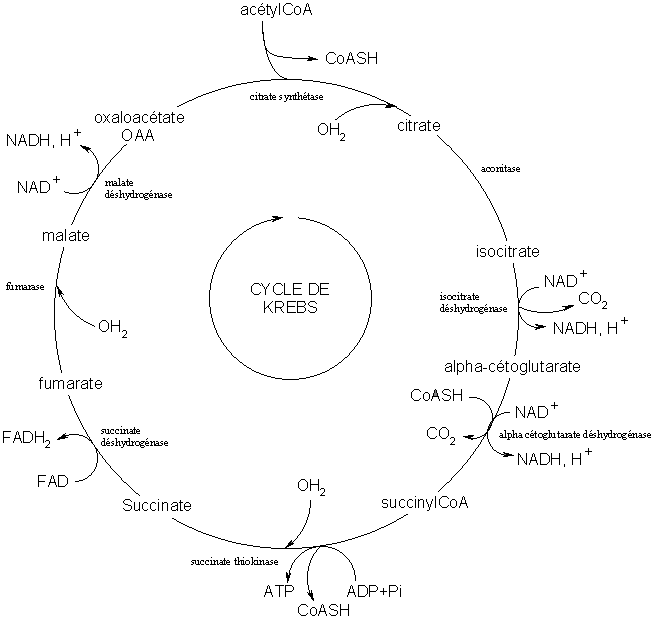
\epsfig {file=img/CycleDeKrebs.png,width=10cm}}
	\caption{Sch{\'e}ma de d{\'e}roulement du cycle de Krebs. }
	\label{fig:cycleDeKrebs}
\end{figure}

\clearpage

\subsection{Mise en place de la programmation}

\subsubsection{Repr{\'e}sentation objet}

\begin{itemize}
	\item Discretisation de l'espace avec des variables d{\'e}finissant des esp{\`e}ces chimiques suivant une nomenclature pr{\'e}-{\'e}tablie (tableau d'ensemble des atomes et mol{\'e}cules). 
	\item D{\'e}finition g{\'e}n{\'e}rique des agents, et {\'e}tablissement {\'e}ventuel de cat{\'e}gories (esp{\`e}ces vivantes et familles, {\'e}l{\'e}ments d'interaction...) avec pour les {\'e}l{\'e}ments vivants ou d{\'e}riv{\'e}s (animaux, plantes, fruits...) une d{\'e}finition d'exp{\`e}ces chimiques ainsi qu'un g{\'e}nome. 
	\item Typage fort des g{\`e}nes (classes de g{\`e}nes, param{\`e}tres, m{\'e}thode d'execution). 
	\item Interactions normalis{\'e}es avec l'environnement (m{\'e}thodes et fonctions de transfert). 
\end{itemize}

\subsubsection{<<Chimie>> -- m{\'e}tabolisme et g{\'e}n{\'e}tique}

\begin{itemize}
	\item \textbf{\emph{Chemicals}}~\\
Ceci d{\'e}signe les variables d'un objet et concerne (avec les g{\`e}nes) les agents actifs comme un organisme ou un {\'e}l{\'e}ment qui en est issu (fruit par exemple). 
	\item \textbf{\emph{Initial Concentration}}~\\
Ce type de g{\`e}ne existe pour initialiser les variables chimiques d'un individu (agent, organisme, \oe uf). 
	\item \textbf{\emph{Biochemical Reaction}}~\\
Les g{\`e}nes de ce type permettent les r{\'e}actions chimiques d'un organisme. 
	\item \textbf{\emph{Emitter}} et \textbf{\emph{Receptor}}~\\
Les g{\`e}nes de ce type permettent l'{\'e}mission et la r{\'e}ception d'{\'e}l{\'e}ments chimiques (ph{\'e}romones). 
	\item \textbf{\emph{Stimulus}, \emph{Decision}, \emph{Brain}, \emph{Lobe}, \emph{Instincts}...}~\\
Il s'agit de g{\`e}nes d'interactions avec l'environnement (\emph{Stimulus}, \emph{Decision}) et de construction de r{\'e}seaux neuronaux d'apprentissage (\emph{Brain}, \emph{Lobe}), dont certains sont pr{\'e}-{\'e}tablis (\emph{Instincts}). 
\end{itemize}

\subsubsection{Interactions entre l'individu et son environnement}

cL'id{\'e}e d'un syst{\`e}me nerveux, minimaliste ou plus {\'e}labor{\'e}, est int{\'e}ressante {\`a} plusieurs titres, notamment pour la mise en place d'un syst{\`e}me de d{\'e}tection (stimulus, sens de perception) ou d'attention et d'action sur des objets. 
	\begin{itemize}
		\item \textbf{\emph{Emetteurs / r{\'e}cepteurs internes et externes}}~\\
Une variation des g{\`e}nes d'{\'e}mission et de r{\'e}ception est possible pour interagir de fa\c{c}on <<chimique>> avec l'environnement, de la m{\^e}me fa\c{c}on que des g{\`e}nes internes le font avec un syst{\`e}me de gestion de la biochimie interne (un syst{\`e}me nerveux). Un exemple de ce type de g{\`e}ne d'action externe est l'{\'e}mission et la d{\'e}tecion de ph{\'e}romones, pour les variants internes il s'agit de boucles d'interactions (variations chimiques plus {\'e}labor{\'e}es que les r{\'e}actions biochimiques). 
		\item \textbf{\emph{Stimuli et d{\'e}cision}}~\\
D{\'e}tection d'{\'e}l{\'e}ments ext{\'e}rieurs {\`a} l'individu (agents dans le m{\^e}me \emph{Container}) et stimulation {\`a} partir de ces {\'e}l{\'e}ments ou de d{\'e}cision d'action sur ces {\'e}l{\'e}ments (r{\'e}cup{\'e}rer, d{\'e}poser, manger, d{\'e}placement...) ; ces g{\`e}nes interc-viennent {\'e}galement sur le syst{\`e}me nerveux. 
		\item \textbf{\emph{Instincts}}~\\
Ce type de g{\`e}nes a pour objectif de cr{\'e}er des connections entre neurones {\`a} partir d'un sch{\'e}ma pr{\'e}-{\'e}tabli et cod{\'e} g{\'e}n{\'e}tiquement, afin de permettre une r{\'e}action directe du syst{\`e}me nerveux d{\`e}s le d{\'e}but (prise de d{\'e}cision suite {\`a} un stimulus). Ceci n'emp{\^e}che pas l'apprentissage de nouveaux sch{\'e}mas lors de la vie de l'individu, ce qui peut servir pour constater l'effet Baldwin~\cite{baldwin1896}. 
		\item \textbf{\emph{Cerveau et lobes}}~\\
L'int{\'e}r{\^e}t de ces types de g{\`e}ne est de r{\'e}server un espace {\`a} un r{\'e}seau de neurones et aux r{\^e}gles qui r{\'e}gissent les neurones (de fa\c{c}on group{\'e}e) afin de cr{\'e}er un ensemble homog{\`e}ne au niveau impl{\'e}mentation, mais potentiellement tr{\`e}s h{\'e}t{\'e}rog{\`e}ne dans ses fonctionnalit{\'e}s. 
	\end{itemize}


\clearpage

\subsubsection{Types d'agents : automates, plantes, bact{\'e}ries, fourmis...}

\begin{itemize}
	\item \underline{\textbf{Automates}} : m{\'e}tabolisme, it{\'e}rations, m{\'e}moire
	\begin{itemize}
		\item \textbf{autoreproducteurs} (copie {\`a} la mutation pr{\`e}s)
		\item \textbf{croiseur/sexu{\'e}} : combine son code avec celui d'un autre (gam{\`e}tes, \oe ufs, copie partielle du g{\'e}nome)
	\end{itemize}

	\item \underline{\textbf{Plantes}} : produisent des fruits, si les fruits ne sont pas consomm{\'e}s, apr{\`e}s un certain d{\'e}lai, une nouvelle plante appara{\^\i}t (dans un premier temps, les plantes ne produisent que des fruits non reproductifs). 

	\item \underline{\textbf{Fourmili{\`e}re}} : reine, \oe ufs, ouvriers, guerriers, reproducteurs ; {\'e}volution des individus ou pr{\'e}-d{\'e}termin{\'e}s ? Ph{\'e}romones (nourriture, contr{\^o}le reproductif...). 
	\begin{itemize}
		\item \textbf{Reine} : ID de la colonie, poss{\`e}de ensemble du g{\'e}nome, produits \oe ufs <<partiels>> selon besoins (nourriture, d{\'e}fense, attaque, colonisation...), 
		\item \textbf{\OE uf} cr{\'e}{\'e} avec une partie d{\'e}termin{\'e}e du g{\'e}nome : donne individu dot{\'e} de fonctions pr{\'e}cises et dot{\'e} d'une vie plus courte. 
		\item \textbf{Ouvrier} : recherche objet (oeuf, nourriture), transport et rassemblement des objets pr{\`e}s de la reine (localisation en m{\'e}moire), laisse des marques (m{\^e}me ID que la reine). 
		\item \textbf{Guerrier} : demande ID, d{\'e}truit agents ayant ID diff{\'e}rent, laisse des marques (m{\^e}me ID que la reine). 
		\item \textbf{Reproducteurs} : voyageur longue distance, m{\^a}le ou femelle (selon moiti{\'e} du g{\'e}nome), s'apparie avec un autre pour donner code entier de nouvelle reine (nouveau ID, mutations, erreurs de coupage de g{\'e}nome, duplication ou d{\'e}l{\'e}tion de g{\`e}ne...). 
	\end{itemize}

	\item \underline{\textbf{R{\'e}seau de fourmilli{\`e}res / mites}} : sur le m{\^e}me principe que la fourmilli{\`e}re pr{\'e}c{\'e}dente, mais les \oe ufs produits donnent des individus qui passent par tous les stades (et finissent par cr{\'e}er de nouvelles colonies).~\\
\end{itemize}

\subsubsection{Codes de transcription, traduction...}

De la m{\^e}me fa\c{c}on que le code g{\'e}n{\'e}tique de traduction antre les acides nucl{\'e}iques et les prot{\'e}ines (un code g{\'e}n{\'e}tique standard et ses variantes selon les Phylum, et Divisions), il est int{\'e}ressant {\`a} plusieurs titres d'encoder <<g{\'e}n{\'e}tiquement>> l'execution des diverses fonctionnalit{\'e}s des Agents (surtout les Organismes). \underline{Le premier int{\'e}r{\^e}t} est que cela permet de d{\'e}finir des fonctions g{\'e}n{\'e}riques pour chacun des types de g{\`e}nes pr{\'e}d{\'e}finis, auquel cas seuls le type de g{\`e}ne et les param{\`e}tres correspondants sont {\`a} encoder (codage param{\'e}trique), la fonction d'un g{\`e}ne {\'e}tant directement executable. \underline{Un autre int{\'e}r{\^e}t} est de transcrire le code {\`a} executer, qui est dynamiquement traduit et {\'e}valu{\'e}, voire compil{\'e} et execut{\'e} si ce code est valable (encodage complet).~\\

De la m{\^e}me fa\c{c}on que le code g{\'e}n{\'e}tique en biologie est redondant, un tel codage informatique peut permettre de r{\'e}duire les effets des mutations, mais un int{\'e}r{\^e}t est d'{\'e}tudier l'impact des mutations et de la s{\'e}lection (tri global et notation par rang des individus de fa\c{c}on aveugle, selon la traduction et l'execution de leur g{\'e}nome). Une telle comparaison entre un g{\'e}nome biologique et un code de programme informatique permettrais de faire {\'e}voluer un code informatique de la m{\^e}me fa\c{c}on qu'une esp{\`e}ce {\'e}volue, non pas dans une recherche de perfection, mais d'optimum dans un environnement donn{\'e} : les outils et m{\'e}thodes  de comparaison et de classification (homologie, phylog{\'e}nie...) peuvent se r{\'e}v{\'e}ler utiles ici {\`a} plusieurs titres pour analyser cette {\'e}volution : FASTA, BLAST, UPGMA, Neighboor-Joining....~\\

Un tel mod{\`e}le de d{\'e}veloppement de simulation, proche des algorithmes g{\'e}n{\'e}tiques, permettrait ainsi d'{\'e}valuer non seulement des mod{\`e}les et simulations biologiques, mais aussi des mod{\`e}les informatiques de programmation (algorithmes, analyses, traitement et {\'e}changes de donn{\'e}es...) dans des contextes donn{\'e}s, selon l'environnement cr{\'e}{\'e} (syst{\`e}me d'exploitation, r{\'e}seau, tests de compatibilit{\'e}s entre programmes) compl{\'e}mentaire des outils existants. 

\clearpage

\section{D{\'e}veloppement}

% \subsubsection{Interface graphique}

% Affichage / vue des cases du monde par un graphisme de 5x5 pixels pour chaque case (une ligne indiquant le type pr{\'e}sent : plante, fruit, fourmis, ph{\'e}romones... ; et la largeur indiquant la quantit{\'e} : 0, 1 {\`a} 5 et plus). Un controleur est pr{\'e}sent pour capturer des {\'e}v{\`e}nements : contr{\^o}le de la mod{\'e}lisation par exemple...

\subsection{Variables, types de g{\`e}nes... Notes d'impl{\'e}mentation. }

\subsubsection{\emph{Chemicals} -- Variables}

Le choix a port{\'e} sur l'int{\'e}gration d'un ensemble de 1000 variables enti{\`e}res, num{\'e}rot{\'e}es de 000 {\`a} 999, accessibles facilement, pour les g{\`e}nes amen{\'e}s {\`a} consulter ou {\`a} modifier ces variables. Les valeurs de ces variables sont initialis{\'e}es {\`a} 0 et sont pr{\'e}vues pour une valeur maximale de 999, ceci dans un soucis de future compatibilit{\'e} lors des enregistrements et de rechargement.

\subsubsection{\emph{GeneHeader} -- En-t{\^e}te}

% longueur :  13 [4 + (3*3)]
Un type g{\'e}n{\'e}rique de g{\`e}nes a {\'e}t{\'e} impl{\'e}ment{\'e}, dont tous les autres g{\`e}nes vont h{\'e}riter, et qui comporte les {\'e}l{\'e}ments d'en-t{\^e}te pour tous les types de g{\`e}nes. Cet en-t{\^e}te comporte des indications sur les possibilit{\'e}s du g{\`e}ne {\`a} muter, {\^e}tre dupliqu{\'e} ou {\`a} {\^e}tre d{\'e}l{\'e}t{\'e}. De plus, des indicateurs fournissent {\'e}galement des informations sur l'activit{\'e} du g{\`e}ne, l'{\^a}ge minimal et l'{\^a}ge maximal d'activation du g{\`e}ne, ainsi que le sexe d'activation (avec une valeur par d{\'e}faut pour activer le g{\`e}ne quelque soit le sexe de l'individu).

\subsubsection{\emph{InitialConcentration} -- Concentrations initiales}

% longueur : 6 [(2*3)]
Le d{\'e}veloppement de ce type de g{\`e}nes est simple, seuls deux param{\`e}tres sont n{\'e}cessaires : la variable {\`a} modifier et la valeur qui doit lui {\^e}tre attribu{\'e}e. Le soucis de compatibilit{\'e} est le m{\^e}me que pour les variables, les param{\`e}tres de ce type de g{\`e}ne vont de 000 {\`a} 999.

\subsubsection{\emph{BiochemicalReaction} -- R{\'e}actions Biochimiques}

% longueur : 27 [(9*3)]
Pour ce type de g{\`e}nes, neuf variables sont n{\'e}cessaires pour indiquer l'ensemble de la r{\'e}action biochimique cod{\'e}e par ce g{\`e}ne. Les param{\`e}tres (dont les valeurs vont de 000 {\`a} 999) sont indiqu{\'e}es avec l'{\'e}quation de la figure~\ref{fig:BiochemicalReactionDescription}. Les r{\'e}actions possibles sont celles du g{\`e}ne correspondant dans \emph{Creatures} et  d{\'e}crites {\`a} la page~\pageref{creatures:reactions}.

\begin{figure}[H]
\begin{center}
\fbox{%
	\begin{minipage}{0.75\linewidth}
		$\mathtt{a * A + b * B \longrightarrow c * C + d * D}$ ; Vitesse de r{\'e}action : $\mathtt{KM}$~\\
		\begin{itemize}
			\item[]	[a-d] $\rightarrow$ [A-D]coef : Coefficient pour le r{\'e}actif [A-D]
			\item[]	[A-D] $\rightarrow$ [A-D]chem : Num{\'e}ro de variable du r{\'e}actif [A-D]
			\item[]	KM $\rightarrow$ KM\_Vmax : Coefficient de vitesse
		\end{itemize}
	\end{minipage}%
}
	\caption[Formule descriptive du g{\`e}ne \emph{BiochemicalReaction}]
	{ Formule descriptive du g{\`e}ne \emph{BiochemicalReaction}~\\
	  \emph{[a-d] indique a, b, c ou d avec respectivement [A-D] indiquant A, B, C ou D.} }
	\label{fig:BiochemicalReactionDescription}
\end{center}
\end{figure}

\subsubsection{\emph{BrainGene} -- Cerveau}

% longueur : 8 [(4*2)] %% WAS %% % longueur : 9 [(3*3)]
Le seul int{\'e}r{\^e}t de ce type g{\`e}ne est de d{\'e}crire la hauteur (\textit{height}), la largeur (\textit{width}) et la profondeur (\textit{depth}) r{\'e}serv{\'e}s aux neurones du syst{\`e}me nerveux. Seules la hauteur et la largeur sont pour l'instant utilis{\'e}es. Tous ces param{\`e}tres sont compris entre 00 et 99. Ce type de g{\`e}ne implique une r{\'e}servation d'espace m{\'e}moire (et de pr{\'e}vision de temps de calcul li{\'e} au r{\'e}seau de neurones) qui est le principal facteur limitant de la simulation, li{\'e} aux calculs n{\'e}cessaires pour les {\'e}tats neuronaux

\subsubsection{\emph{BrainLobeGene} -- Lobes du cerveau}

% longueur : 36 [(11*3)+3]
Ce type de g{\`e}ne d{\'e}crit la position (coordonn{\'e}es x et y), la hauteur et la largeur des lobes au sein du cerveau (si celui-ci est pr{\'e}alablement d{\'e}finit avec un g{\`e}ne correspondant) et ont des valeurs entre 000 et 999. D'autres param{\`e}tres sont {\'e}galement dans ce type de g{\`e}ne et concernent les propri{\'e}t{\'e}s des neurones contenus dans ce lobe, le niveau de repos, le niveau d'activation, la valeur de diminution, le nombre minimal et le nombre maximal de dendrite, la proximit{\'e} des connnexions {\'e}tablies, la possibilit{\'e} de reproduction des neurones et l'indication si le lobe contient un seul neurone actif ou non (comportment WTA).~\\

Les neurones sont totalement configurables dans leur comportement au sein des lobes de fa\c{c}on isol{\'e}e ou globalement (lobes d'un seul neurone, comportment WTA du lobe, nombre de connexions...). L'int{\'e}r{\^e}t est de pouvoir grouper les neurones selon l'int{\'e}r{\^e}t de leur activit{\'e} et de la gestion des entr{\'e}es et des sorties du cerveau, associ{\'e}s {\`a} des g{\`e}nes {\'e}metteurs-r{\'e}cepteurs ou de stimulus. 

\subsubsection{\emph{EmitterReceptor} -- {\'E}metteurs et r{\'e}cepteurs}

% longueur : 15 [(3*3) + (2*2) + 2]
L'int{\'e}r{\^e}t de ce type de g{\`e}ne est l'interaction des variables chimiques avec le syst{\`e}me nerveux d'un organisme donn{\'e}, soit pour indiquer l'atteinte d'un seuil chimique (r{\'e}cepteur) soit pour {\'e}mettre une esp{\`e}ce chimique {\`a} la demande ({\'e}metteur). Ceci s'effectue prioritairement sur les variables chimiques internes {\`a} l'organisme ; ensuite l'int{\'e}r{\^e}t des ph{\'e}romones sur leur d{\'e}p{\^o}t et leur d{\'e}tection a amen{\'e} {\`a} {\'e}largir leur effet aux variables de l'environnement courant ({\'e}metteurs et r{\'e}cepteurs externes dans ce cas). Les variables de ce type de g{\`e}ne sont le num{\'e}ro de la variable concern{\'e}e, le niveau d'activation (du neurone ou de la variable chimique), la valeur {\`a} ajouter ({\`a} la variable ou {\`a} l'{\'e}tat du neurone), la position du neurone, un indicateur <<{\'e}metteur ou r{\'e}cepteur>> et un indicateur pour en conna{\^\i}tre l'internalit{\'e}.~\\

Les {\'e}metteurs et les r{\'e}cepteurs peuvent {\^e}tre amen{\'e}s {\`a} avoir un r{\^o}le mineur dans le fonctionnement du syst{\`e}me nerveux, en-dehors des signaux li{\'e}s {\`a} la pr{\'e}sence de ph{\'e}romones (contact avec les variables ext{\'e}rieures locales). Une application interne du syst{\`e}me nerveux est l'intervention de boucles de r{\'e}tro-action (\emph{loopback}) dans l'organisme concern{\'e} pour provoquer certaines r{\'e}actions chimiques ou certains comportements complexes. 

\subsubsection{\emph{StimulusDecision} -- Perception et d{\'e}cision}

% longueur : 20 [2 + (6*3)]
Ce type de g{\`e}ne est proche du type \emph{EmitterReceptor} sur le principe de base : il s'agit de recevoir des donn{\'e}es et de les int{\'e}grer aux variables ou d'accomplir des actions en fonctions des variables. Les param{\`e}tres de ce type de g{\`e}ne sont : l'indicateur d'entr{\'e}e ou de sortie (perception ou d{\'e}cision), un indicateur de variable ou d'objet (liste pr{\'e}-{\'e}tablie), le num{\'e}ro de variable ou d'objet source (de 000 {\`a} 999), le seuil d'activation, un attribut (direction, type d'objet, {\'e}tat), la variable destination, la valeur {\`a} ajouter dans cette variable et l'action {\`a} effectuer.~\\

Un parcours global de ce type de g{\`e}ne est n{\'e}cessairement reli{\'e} {\`a} une m{\'e}moire (une partie des variables), pour la partie de \emph{prise en compte des d{\'e}cisions} dont la prise en compte est d{\'e}coupl{\'e}e de la g{\'e}n{\'e}tique, mais aussi pour la r{\'e}ception des stimulus. Cette m{\'e}moire indique les actions {\`a} accomplir avec {\'e}ventuellement certains param{\`e}tres associ{\'e}s (direction, objet) et est d{\'e}crite page~\pageref{tab:NomenclatureStimuliDecision}.~\\

L'int{\'e}r{\^e}t d'un typage fort et d'une nomenclature des objets et des directions dans l'environnement est n{\'e}cessaire {\`a} ce niveau, ceci permet notamment la d{\'e}tection de ph{\'e}romone dans des cases voisines. Ce type de g{\`e}ne n'est pas obligatoirement li{\'e} {\`a} un syst{\`e}me nerveux, mais peut l'{\^e}tre via les g{\`e}nes \emph{EmitterReceptor}. Dans ce cas, un lobe d'attention et de d{\'e}cision utilise la fonctionnalit{\'e} \emph{WTA} des lobes pour assurer un r{\'e}sultat d'attention ou d'action unique. 

\subsubsection{\emph{Instinct} -- R{\'e}seaux neuronaux pr{\'e}-{\'e}tablis}

% longueur : 18 [(6*3)]
L'objectif de ce type de g{\`e}nes est d'{\'e}tablir des connexions entre neurones au sein du syst{\`e}me nerveux des individus. Pour que ces connexions s'{\'e}tablissent {\`a} certains stades de la vie de l'individu et pour {\'e}viter une concurrence {\'e}ventuelle avec d'autres constructions neuronales au cours de la vie de l'individu, ce type de g{\`e}ne d{\'e}pend d'une variable chimique d{\'e}finie qui diminue {\`a} l'usage. Les variables de ce type de g{\`e}nes sont : la variable utilis{\'e}e, la quantit{\'e} utilis{\'e}e, les coordonn{\'e}es du neurone de d{\'e}part, les coordonn{\'e}es du neurone d'arriv{\'e}e et le poid de la connexion. Si la connexion existe d{\'e}j{\`a} et que la variable chimique est encore pr{\'e}sente, la connexion est simplement renforc{\'e}e.~\\

L'int{\'e}r{\^e}t principal de la pr{\'e}sence de ce type de g{\`e}ne est de construire certains comportements quelque soit la complexit{\'e} du syst{\`e}me nerveux de l'organsime : le nombre de g{\`e}nes de ce type est bien s{\^u}r d{\'e}pendant de la complexit{\'e} des comportments {\`a} obtenir et des concepts au sein du r{\'e}seau de neurones et des connexions {\`a} construire entre neurones. 

\clearpage

L'utilisation d'une variable chimique d{\'e}termin{\'e}e pour le fonctionnement de ce g{\`e}ne entra{\^\i}ne une d{\'e}pendance {\`a} la pr{\'e}sence du compos{\'e}, de pr{\'e}f{\'e}rence par l'utilisation d'un g{\`e}ne \emph{InitialConcentration} pour un d{\'e}veloppement des connexion dans les premiers stades de la vie de l'individu ; {\'e}ventuellement, cela peut intervenir au cours de la vie de l'individu par l'apparition du compos{\'e} suite un g{\`e}ne \emph{BiochemicalReaction}ou un g{\`e}ne \emph{EmitterReceptor})...


\subsection{Liste normalis{\'e}e des <<{\'e}l{\'e}ments chimiques>>}

Par convention, le premier {\'e}l{\'e}ment de cette liste normalis{\'e}e (tableau~\ref{tab:NomenclatureBiochimie}) {\`a} la position \emph{000} est \emph{<NONE00>}, tous les autres {\'e}l{\'e}ments <<non attribu{\'e}s>> sont nomm{\'e}s de la m{\^e}me fa\c{c}on entre chaque groupe d'{\'e}l{\'e}ments d{\'e}finis. Les {\'e}l{\'e}ments \emph{001} {\`a} \emph{118} symbolisent directement la chimie de base, sans prendre en compte les isotopes {\'e}ventuels. Les {\'e}l{\'e}ments {\`a} partir de \emph{151} symbolisent des mol{\'e}cules de biochimie classique (acides amin{\'e}s, nucl{\'e}otides, acides gras, sucres...) ; puis {\`a} partir de \emph{600}, les hormones, et {\`a} partir de \emph{651}, les ph{\'e}romones. \textit{Les {\'e}l{\'e}ments {\`a} partir de \emph{800} sont utilis{\'e}s par le r{\'e}seau neuronal et seront d{\'e}taill{\'e} dans le tableau~\ref{tab:NomenclatureStimuliDecision}. }

%% 
\def\titreNormalise{Nomenclature des variables de chimie et biochimie}
%% 

\begin{scriptsize}
\begin{longtable}{|>{\columncolor{verylightgray}}p{0.04\textwidth}|p{0.16\textwidth}|>{\columncolor{verylightgray}}p{0.04\textwidth}|p{0.16\textwidth}|>{\columncolor{verylightgray}}p{0.04\textwidth}|p{0.16\textwidth}|>{\columncolor{verylightgray}}p{0.04\textwidth}|p{0.16\textwidth}|}
	\hline \rowcolor[gray]{0.50} \multicolumn{8}{|c|}{\titreNormalise} \\ \hline
	\endfirsthead
	\hline \rowcolor[gray]{0.50} \multicolumn{8}{|c|}{\titreNormalise (suite)} \\ \hline
	\endhead
	\hline \multicolumn{8}{|c|}{... Suite page suivante ...} \\ \hline
	\endfoot
	\hline
	\endlastfoot
	% \centering
%%%%% \rowcolor{--} ne marche pas sur les multicolumn !!
	\multicolumn{8}{|>{\columncolor{lightgray}}c|}{Liste des atomes (table p{\'e}riodique des {\'e}l{\'e}ments)} \\ \hline
	% \rowcolor{white}
	001 & H	Hydrogen			& 031 & Ga	Gallium			& 061 & Pm	Promethium		& 091 & Pa	Proctatinium	\\ \hline
	002 & He	Helium			& 032 & Ge	Germanium		& 062 & Sm	Samarium		& 092 & U	Uranium 		\\ \hline
	003 & Li	Lithium			& 033 & As	Arsenic			& 063 & Eu	Europium		& 093 &  Np	Neptunium		\\ \hline
	004 & Be	Beryllium		& 034 & Se	Selenium		& 064 & Gd	Gadolnium		& 094 & Pu	Plutonium 		\\ \hline
	005 & B	Bore				& 035 & Br	Brome			& 065 & Tb	Terbium			& 095 & Am	Americanium 	\\ \hline
	006 & C	Carbon				& 036 & Kr	Krypton			& 066 & Dy	Dysprosium		& 096 & Cm	Curium 			\\ \hline
	007 & N	Azote				& 037 & Rb	Rubidium		& 067 & Ho	Holmium			& 097 & Bk	Berkelium 		\\ \hline
	008 & O	Oxygen				& 038 & Sr	Strontium		& 068 & Er	Erbium			& 098 & Cf	Californium 	\\ \hline
	009 & F	Fluor				& 039 & Y	Yttirum			& 069 & Tm	Thulium			& 099 & Es	Einsteinium 	\\ \hline
	010 & Ne	Neon			& 040 & Zr	Zirconium		& 070 & Yb	Ytterbium		& 100 & Fm	Fermium 		\\ \hline
	011 & Na	Sodium			& 041 & Nb	Niobium			& 071 & Lu	Lut{\'e}cium	& 101 & Md	Mendelevium 	\\ \hline
	012 & Mg	Magnesium		& 042 & Mo	Molybdene		& 072 & Hf	Hafnium			& 102 & No	Nobelium 		\\ \hline
	013 & Al	Aluminium		& 043 & Tc	Technetium		& 073 & Ta	Tantale			& 103 & Lr	Lawrencium 		\\ \hline
	014 & Si	Silicium		& 044 & Ru	Ruthenium		& 074 & W	Tungst{\`e}ne	& 104 & Rf	Rutherfordium 	\\ \hline
	015 & P	Phosphor			& 045 & Rh	Rhodium			& 075 & Re	Rhenium 		& 105 & Db	Dubnium 		\\ \hline
	016 & S	Soufre				& 046 & Pd	Palladium		& 076 & Os	Osmium 			& 106 & Sg	Seaborgium 		\\ \hline
	017 & Cl	Chlore			& 047 & Ag	Argent			& 077 & Ir	Iridium 		& 107 & Bh	Bohrium 		\\ \hline
	018 & Ar	Argon			& 048 & Cd	Cadmium			& 078 & Pt	Platinium 		& 108 & Hs	Hassium 		\\ \hline
	019 & K	Potassium			& 049 & In	Indium			& 079 & Au	Auri -- Or 		& 109 & Mt	Meitnerium 		\\ \hline
	020 & Ca	Calcium			& 050 & Sn	Sin (Etain)		& 080 & Hg	Mercure 		& 110 & Ds	Darmstatdium 	\\ \hline
	021 & Sc	Scandium		& 051 & Sb	Stibium 		& 081 & Tl	Thallium		& 111 & Rg	Roentgenium 	\\ \hline
	022 & Ti	Titanium		& 052 & Te	Tellurium		& 082 & Pb	Plomb			& 112 & Cn	Copernicium 	\\ \hline
	023 & V	Vanadium			& 053 & I	Iodine (Iode)	& 083 & Bi	Bismuth			& 113 & Uut	Uut 			\\ \hline
	024 & Cr	Chrome			& 054 & Xe	Xenon			& 084 & Po	Polonium		& 114 & Uuq	Uuq 			\\ \hline
	025 & Mn	Manganese		& 055 & Cs	Caesium			& 085 & At	Astate			& 115 & Uup	Uup 			\\ \hline
	026 & Fe	Fer				& 056 & Ba	Barium			& 086 & Rn	Radon			& 116 & Uuh	Uuh 			\\ \hline
	027 & Co	Cobalt			& 057 & La	Lanthane		& 087 & Fr	Francium		& 117 & Uus	Uus 			\\ \hline
	028 & Ni	Nickel			& 058 & Ce	Cerium			& 088 & Ra	Radium			& 118 & Uuo	Uuo 			\\ \hline
	029 & Cu	Cuivre			& 059 & Pr	Praseodyne		& 089 & Ac	Actinium		& 119 & \emph{<NONE01>}		\\ \hline
	030 & Zn	Zinc			& 060 & Nd	Neodyme			& 090 & Th	Thorium			& 120 & \emph{<NONE02>} 	\\ \hline
	\hline
	\pagebreak[3]
	\multicolumn{8}{|>{\columncolor{lightgray}}c|}{Hormones (600 et plus) et Ph{\'e}romones (650 et plus)} \\ \hline
	% \rowcolor{white}
	\textbf{600} & Hormone00	& 605 & Hormone05		& \textbf{650} & Pheromone00 	& 655 & Pheromone05 \\ \hline
	601 & Progesterone			& 606 & Hormone06		& 651 & Pheromone01 			& 656 & Pheromone06 \\ \hline
	602 & Oestrogene			& 607 & Hormone07		& 652 & Pheromone02 			& 657 & Pheromone07 \\ \hline
	603 & Testosterone			& 608 & Hormone08		& 653 & Pheromone03 			& 658 & Pheromone08 \\ \hline
	604 & Hormone04				& 609 & Hormone09		& 654 & Pheromone04 			& 659 & Pheromone09 \\ \hline
	\hline
	\pagebreak[3]
	\multicolumn{8}{|>{\columncolor{lightgray}}c|}{Mol{\'e}cules biochimiques complexes ({\`a} partir de 151)} \\ \hline
	% \rowcolor{white}
	150 & \emph{<NONE31>}		& 183 & H$_2$O				& 216 & AAE	Glutamate			& 249 & Acide Pelargonique			\\ \hline
	151 & \textbf{ATP}			& 184 & Hydroxyd (OH$^-$)	& 217 & AAQ	Glutamine			& 250 & Acide Caprique				\\ \hline
	152 & ADP					& 185 & \textbf{AcetylCoA}	& 218 & AAG	Glycine				& 251 & Acide Undecylique			\\ \hline
	153 & AMP					& 186 & OxaloAcetate		& 219 & AAH	Histidine			& 252 & Acide Laurique				\\ \hline
	154 & CTP					& 187 & \textbf{Citrate}	& 220 & AAI	IsoLeucine 			& 253 & Acide Tridecylique			\\ \hline
	155 & CDP					& 188 & CoASH				& 221 & AAL	Leucine				& 254 & Acide Myristique			\\ \hline
	156 & CMP					& 189 & cis-Aconitate		& 222 & AAK	Lysine 				& 255 & Acide Pentadecyl.			\\ \hline
	157 & GTP					& 190 & iso-Citrate			& 223 & AAM	Methionine			& 256 & Acide Palmitique			\\ \hline
	158 & GDP					& 191 & Oxalosuccinate		& 224 & AAF	PhenylAlanine 		& 257 & Acide Margarique			\\ \hline
	159 & GMP					& 192 & alpha-Cetoglutarate	& 225 & AAP	Proline				& 258 & Acide Stearique				\\ \hline
	160 & TTP					& 193 & SuccinylCoA			& 226 & AAO	Pyrolysine			& 259 & Acide Nonadecyl.			\\ \hline
	161 & TDP					& 194 & Succinate			& 227 & AAU	SelenoCyst.			& 260 & Acide Arachidique			\\ \hline
	162 & TMP					& 195 & Fumarate			& 228 & AAS	Serine 				& 261 & Acide h{\'e}n{\'e}icosan.	\\ \hline
	163 & UTP					& 196 & Malate				& 229 & AAT	Threonine			& 262 & Acide B{\'e}h{\'e}nique		\\ \hline
	164 & UDP					& 197 & CyclicElement02		& 230 & AAW	Tryptophane			& 263 & Acide tricosanoique			\\ \hline
	165 & UMP					& 198 & CyclicElement01		& 231 & AAY	Tyrosine			& 264 & Acide Lignocerique			\\ \hline
	166 & NAD					& 199 & \textbf{Pyruvate}	& 232 & AAV	Valine 				& 265 & Acide pentacosan.			\\ \hline
	167 & NADH,H$^+$			& 200 & \textbf{Adenine}	& 233 & \emph{AminoAcid00}		& 266 & Acide C{\'e}rotique			\\ \hline
	168 & FAD					& 201 & Cytosine			& 234 & \emph{AminoAcid01}		& 267 & Acide heptacosan.			\\ \hline
	169 & FADH2					& 202 & Guanine				& 235 & \emph{AminoAcid02}		& 268 & Acide Montanique			\\ \hline
	170 & Glucose				& 203 & Thymin				& 236 & \emph{AminoAcid03}		& 269 & Acide nonacosan.			\\ \hline
	171 & Fructose				& 204 & Uracil				& 237 & \emph{AminoAcid04}		& 270 & Acide Melissique			\\ \hline
	172 & Glucose-6-P			& 205 & \emph{BasicMole00}	& 238 & \emph{AminoAcid05}		& 271 & Acide hentriaco.			\\ \hline
	173 & Fructose-6-P			& 206 & \emph{BasicMole01}	& 239 & \emph{AminoAcid06}		& 272 & Acide Laceroique			\\ \hline
	174 & Fructose-1,6-biP.		& 207 & \emph{BasicMole02}	& 240 & \emph{AminoAcid07}		& 273 & \emph{FattyAcid00} (33c)	\\ \hline
	175 & DHAP					& 208 & \emph{BasicMole03}	& 241 & \textbf{Acide Formique}	& 274 & \emph{FattyAcid01} (34c)	\\ \hline
	176 & PGAL					& 209 & \emph{BasicMole04}	& 242 & Acide Ac{\'e}tique		& 275 & \emph{FattyAcid02} (35c)	\\ \hline
	177 & BisphosphoGlycerate	& 210 & \emph{BasicMole05}	& 243 & Acide Propionique	 	& 276 & \emph{FattyAcid03} (36c)	\\ \hline
	178 & 3-PhosphoGlycerate	& 211 & AAA	Alanine			& 244 & Acide Butyrique		 	& 277 & \emph{FattyAcid04} (37c)	\\ \hline
	179 & 2-PhosphoGlycerate	& 212 & AAR	Arginine		& 245 & Acide Valerique		 	& 278 & \emph{FattyAcid05} (38c)	\\ \hline
	180 & phosphoenolPyruvate	& 213 & AAN	Asparagine		& 246 & Acide Caproique		 	& 279 & \emph{FattyAcid06} (39c)	\\ \hline
	181 & O$_2$					& 214 & AAD	Aspartate		& 247 & Acide Enanthique		& 280 & \emph{FattyAcid07} (40c)	\\ \hline
	182 & CO$_2$				& 215 & AAC	Cysteine		& 248 & Acide Pelargonique		& 281 & \emph{<NONE00>}				\\ \hline
	\caption[Nomenclature des variables de chimie et biochimie]
		{Nomenclature des variables de chimie et biochimie \emph{} }
	\label{tab:NomenclatureBiochimie}
\end{longtable}
\end{scriptsize}
~\\
% \clearpage
% \subsection{Encodage des identifications : objets, environnement...}


\begin{table}[ht]
	\scriptsize
	\centering 
\begin{tabular}{|>{\columncolor{verylightgray}}p{0.05\textwidth}|p{0.20\textwidth}||>{\columncolor{verylightgray}}p{0.05\textwidth}|p{0.20\textwidth}||>{\columncolor{verylightgray}}p{0.05\textwidth}|p{0.20\textwidth}|}
\hline
%%%%% \rowcolor{--} ne marche pas sur les multicolumn !!
	\multicolumn{6}{|>{\columncolor{lightgray}}c|}{Encodage des directions (800 -- 829)} \\ \hline
	% \rowcolor{white}
			800 & (local) 	(LLL)	&	810 & Up (UUU)		&	820 & Down (DDD) 	\\ \hline
			801 & NorthWest (LNW)	&	811 & (UNW)			&	821 & (DNW)  		\\ \hline
			802 & North 	(LNN)	&	812 & (UNN)			&	822 & (DNN)  		\\ \hline
			803 & NorthEast (LNE)	&	813 & (UNE)			&	823 & (DNE)  		\\ \hline
			804 & East 	(LEE)		&	814 & (UEE)			&	824 & (DEE)  		\\ \hline
			805 & SouthEast (LSE)	&	815 & (USE)			&	825 & (DSE)  		\\ \hline
			806 & South	(LSS)		&	816 & (USS)			&	826 & (DSS)  		\\ \hline
			807 & SouthWest (LSW)	&	817 & (USW)			&	827 & (DSW)  		\\ \hline
			808 & West	(LWW)		&	818 & (UWW)			&	828 & (DWW)  		\\ \hline
	% 		809 & (free)			&	819 & (free)		&	829 & (free)  		\\ \hline
	\hline
	\multicolumn{6}{|>{\columncolor{lightgray}}c|}{Encodage des stimuli et d{\'e}cisions (851 -- 880)} \\ \hline
	% \rowcolor{white}
			851 & Stay 			&	861 & Rest			&	871 & Mate		\\ \hline
			852 & Push(x)		&	862 & Sleep			&	872 & (free)	\\ \hline
			853 & Pull(x)		&	863 & Eat			&	873 & (free)	\\ \hline
			854 & Stop 			&	864 & Death			&	874 & (free)	\\ \hline
			855 & Move to(x)	&	865 & Emit(x)		&	875 & (free)	\\ \hline
			856 & Move away		&	866 & Receive(x)	&	876 & (free)	\\ \hline
			857 & Get(x)		&	867 & Has(x)		&	877 & (free)	\\ \hline
			858 & Drop(x)		&	868 & Is(x)			&	878 & (free)	\\ \hline
			859 & Think(x)		&	869 & MakeGamet		&	879 & (free)	\\ \hline
			860 & Slap(x)		&	870 & LayEgg		&	880 & (free)	\\ \hline
	\hline
	\multicolumn{6}{|>{\columncolor{lightgray}}c|}{Encodage des objets et des {\'e}tats} \\ \hline
	% \rowcolor{white}
			900 & Current		&	920 & Gamet		&	940 & Gender (sex)	\\ \hline
			901 & Small elt		&	921 & Egg		&	941 & Aging			\\ \hline
			902 & Midd elt		&	922 & Embryo	&	942 & TypeOf		\\ \hline
			903 & Big elt		&	923 & Larva		&	943 & Movable		\\ \hline
			904 & Food 			&	924 & Child		&	944 & Eatable		\\ \hline
			905 & Drink			&	925 & ``Teen''	&	945 & Fertile		\\ \hline
			906 & Vehicle		&	926 & Adult		&	946 & Pregnant		\\ \hline
			907 & Automaton		&	927 & Senior	&	947 & (free)		\\ \hline
			908 & Computer		&	928 & Dead		&	948 & (free)		\\ \hline
			909 & Laptop		&	929 & (free)	&	949 & (free)		\\ \hline
			910 & Phone			&	930 & (free)	&	950 & (free)		\\ \hline
			911 & Cell Phone	&	931 & (free)	&	951 & (free)		\\ \hline
			912 & Ant			&	932 & (free)	&	952 & (free)		\\ \hline
			913 & (free)		&	933 & (free)	&	953 & (free)		\\ \hline
			914 & (free)		&	934 & (free)	&	954 & (free)		\\ \hline
			915 & (free)		&	935 & Daemon	&	955 & (free)		\\ \hline
			916 & (free)		&	936 & Bacta		&	956 & (free)		\\ \hline
			917 & (free)		&	937 & Plant		&	957 & (free)		\\ \hline
			918 & (free)		&	938 & Anima		&	958 & (free)		\\ \hline
			919 & (free)		&	939 & Virus		&	959 & (free)		\\ \hline
			\hline
		\end{tabular}
	\caption[Nomenclature pour les Stimuli et D{\'e}cisions]
		{ Nomenclature pour les Stimuli et D{\'e}cisions~\\
Cette partie de la nomenclature concerne une utilisation (interne ou externe) par les g{\`e}nes de type \emph{StimulusDecision} et \emph{EmitterReceptor}. \emph{Seules les 9 premi{\`e}res directions sont utilis{\'e}es. L'action 864 entra{\^\i}ne la mort de l'agent courant, les {\'e}tats {\`a} partir de 940 le d{\'e}crivent. }}
	\label{tab:NomenclatureStimuliDecision}
\end{table}

% Certains {\'e}tats (940 et plus) sont utiles de fa\c{c}on g{\'e}n{\'e}rale pour un agent donn{\'e}. 

% \subsection{Sorties du syst{\`e}me nerveux : attention, decision, direction...}

\clearpage

\subsection{Encodage g{\'e}n{\'e}tique}

\subsubsection{G{\`e}nes <<param{\`e}tres>> -- \emph{GeneGattaca}}

Dans ce cas les g{\`e}nes sont des fonctions pr{\'e}-encod{\'e}es comme dans \textit{Creatures}, avec des param{\`e}tres susceptibles de varier ; les variables sont num{\'e}rot{\'e}es de 000 {\`a} 999 ; les g{\`e}nes sont fortement typ{\'e}s (regroup{\'e}s sous le terme \emph{GeneGattaca}). L'{\'e}criture des g{\`e}nes est d{\'e}finie par l'ordre des param{\`e}tres et utilisera le code d{\'e}crit dans le tableau~\ref{tab:InformationGenetiqueTripletsParametres} lors de sauvegarde externes. Ces g{\`e}nes sont d{\'e}finis comme commen\c{c}ant avec ``M'' et finissant avec ``*''. Afin de permettre une lisibilit{\'e} humaine, l'id{\'e}e de base est de les encoder ligne par ligne.~\\

Lors d'un chargement dans le mod{\`e}le, les g{\`e}nes cr{\'e}{\'e}s avec le codage param{\'e}trique sont traduits et reconnus en fonction de leur longueur (nombre de caract{\`e}res n{\'e}cessaires pour les param{\`e}tres), puis sont charg{\'e}s en m{\'e}moire. 

\begin{table}[h]
	\begin{tabular}{p{0.40\textwidth} p{0.60\textwidth}} % \begin{center} % ||
	\begin{tabular}{p{0.40\textwidth}}
		% \begin{small}
		\emph{Les  param{\`e}tres des g{\`e}nes sont cod{\'e}s selon les modes suivants : les \textbf{\emph{bool{\'e}ens}} sont des chiffres soient pairs (\textbf{true} -- vrai) soient impairs (\textbf{false} -- faux), les \textbf{\emph{valeurs num{\'e}riques}} sont rep{\'e}r{\'e}es et regroup{\'e}es lin{\'e}rairement selon le nombre de chiffres n{\'e}cessaires et traduits pour dans le sens de lecture (de gauche {\`a} droite) par des puissances d{\'e}croissantes de dix, jusqu'{\`a} l'unit{\'e}. Dans le cas d'un param{\`e}tre d{\'e}finis par un nombre {\`a} trois chiffres, le premier chiffre lu est celui des centaines, puis le second celui des dizaines, et enfin celui des unit{\'e}s.}~\newline

\emph{Le code est redondant pour les chiffres  car ce les plus utilis{\'e}s dans les param{\`e}tres, les lettres sont l{\`a} pour construire les annotations avec les s{\'e}parateurs $:$ et $'$.}
		%\end{small}
		\\
	\end{tabular} 
	&
	\begin{tabular}{|>{\columncolor{verylightgray} }c|>{\columncolor{white}}p{0.05\textwidth}||>{\columncolor{verylightgray} }c|>{\columncolor{white}}p{0.05\textwidth}||>{\columncolor{verylightgray} }c|>{\columncolor{white}}p{0.05\textwidth}||>{\columncolor{verylightgray}
}c|>{\columncolor{white}}p{0.05\textwidth}|}
		\hline
aaa	& a	& caa	& q	& taa	& 2	& gaa	& 7 \\ \hline %  & & 
aac	& b	& cac	& r	& tac	& 2	& gac	& 7 \\ \hline
aat	& c	& cat	& s	& tat	& 2	& gat	& 8 \\ \hline
aag	& d	& cag	& t	& tag	& 3	& gag	& 8 \\ \hline
aca	& e	& cca	& u	& tca	& 3	& gca	& 8 \\ \hline
acc	& f	& ccc	& v	& tcc	& 3	& gcc	& 9 \\ \hline
act	& g	& cct	& w	& tct	& 4	& gct	& 9 \\ \hline
acg	& h	& ccg	& x	& tcg	& 4	& gcg	& 9 \\ \hline
ata	& i	& cta	& y	& tta	& 4	& gta	& $:$ \\ \hline
atc	& j	& ctc	& z	& ttc	& 5	& gtc	& $:$ \\ \hline
att	& k	& ctt	& 0	& ttt	& 5	& gtt	& $'$ \\ \hline
atg	& l	& ctg	& 0	& ttg	& 5	& gtg	& $'$ \\ \hline
aga	& m	& cga	& 0	& tga	& 6	& gga	& $M$ \\ \hline
agc	& n	& cgc	& 1	& tgc	& 6	& ggc	& $M$ \\ \hline
agt	& o	& cgt	& 1	& tgt	& 6	& ggt	& $*$ \\ \hline
agg	& p	& cgg	& 1	& tgg	& 7	& ggg	& $*$ \\ \hline 
\hline \hline
\multicolumn{8}{|c|}{ \emph{$M$ indique les codons start et $*$ les codons stop. }} \\ \hline
		\end{tabular} \\
	\end{tabular} % \end{center}
	\caption[Les 64 triplets du codage param{\'e}trique \emph{GeneGattaca}]{Les 64 triplets du codage param{\'e}trique \emph{GeneGattaca}}%~\newline \emph{--}}
	\label{tab:InformationGenetiqueTripletsParametres}
\end{table}

\begin{tabular}{p{0.40\textwidth} p{0.30\textwidth} p{0.30\textwidth}}
	\begin{tabular}{p{0.40\textwidth}}
		L'en-t{\^e}te des g{\`e}nes (\textbf{\emph{header}}) est d{\'e}fini pour l'ensemble des types de g{\`e}nes avec les param{\`e}tres suivants (15 caract{\`e}res) : \\
	\end{tabular} &

	\begin{tabular}{p{0.30\textwidth}}
		\begin{itemize}
			\item mutate (bool{\'e}en)
			\item duplicate (bool{\'e}en)
			\item delete (bool{\'e}en)
			\item activ (bool{\'e}en)
		\end{itemize} \\
	\end{tabular} &
	
	\begin{tabular}{p{0.30\textwidth}}
		\begin{itemize}
			\item ageMin (000 {\`a} 999)
			\item ageMax (000 {\`a} 999)
			\item sex (000 {\`a} 9999)
			\item mutRate (00 {\`a} 99)
		\end{itemize}\\
	\end{tabular} \\
\end{tabular}

Les types de g{\`e}nes cr{\'e}{\'e}s avec ce code (\emph{GeneGattaca}) sont d{\'e}crits, avec leurs param{\`e}tres et valeurs possibles, dans le tableau~\ref{tab:briefDescriptionGeneTypes}. Un attribut compl{\'e}mentaire (\textit{more}) a {\'e}t{\'e} ajout{\'e} au \emph{BrainGene} pour {\'e}viter une confusion avec \emph{InitialConcentration} dans la longueur du g{\`e}ne d{\'e}crit.~\\

D'autres types de g{\`e}nes peuvent {\^e}tre d{\'e}velopp{\'e}s au-del{\`a} de cette base de g{\`e}nes param{\'e}triques, comme les g{\`e}nes de transposition ou les g{\`e}nes viraux. L'id{\'e}e initiale de ces g{\`e}nes est de provoquer des comportements particuliers au niveau des g{\'e}nomes et de la biochimie des organismes mod{\'e}lis{\'e}s. Dans le cas des transposons, il suffit de d{\'e}placer des g{\`e}nes au sein du g{\'e}nome d'un organisme : l'ordre d'execution des g{\`e}nes dans le mod{\`e}le peut avoir un avantage {\'e}volutif. Concernant les g{\`e}nes viraux, l'objectif est le d{\'e}tournement du m{\'e}tabolisme h{\^o}te pour produire de nouvelles particules virales. \emph{\textbf{Dans ces deux cas, g{\`e}nes viraux et transposons, en plus des g{\`e}nes d{\'e}j{\`a} {\'e}tablis, un seul type de g{\`e}ne param{\'e}trique est {\`a} ajouter : des g{\`e}nes de modification du g{\'e}nome au niveau des g{\`e}nes (insertion, d{\'e}l{\'e}tion, r{\'e}arrangement).}}~\\

\clearpage

\begin{table}[h]
	\begin{center} \begin{scriptsize}
	\begin{tabular}{|p{0.25\textwidth}|c|p{0.25\textwidth}|p{0.25\textwidth}|}
\hline
	\rowcolor{lightgray} Type	& Longueur	& Param{\`e}tre	& Valeurs \\ \hline
	InitialConcentration		&	6 (2*3)		&	variable	& [000-999] \\
	\cline{3-4} % \hline
								&				&	value		& [000-999] \\
	\hline \hline
	BiochemicalReaction			&	27 (9*3)	&	Achem		& [000-999] \\
	\cline{3-4} % \hline
								&				&	Acoef		& [000-999] \\
	\cline{3-4} % \hline
								&				&	Bchem		& [000-999] \\
	\cline{3-4} % \hline
								&				&	Bcoef		& [000-999] \\
	\cline{3-4} % \hline
								&				&	Cchem		& [000-999] \\
	\cline{3-4} % \hline
								&				&	Ccoef		& [000-999] \\
	\cline{3-4} % \hline
								&				&	Dchem		& [000-999] \\
	\cline{3-4} % \hline
								&				&	Dcoef		& [000-999] \\
	\cline{3-4} % \hline
								&				&	KM			& [000-999] \\
	\hline \hline
	BrainGene					&	8 (4*2)		&	height		& [00-99] \\
	\cline{3-4} % \hline
								&				&	width		& [00-99] \\
	\cline{3-4} % \hline
								&				&	\textit{depth}	& [00-99] \\
	\cline{3-4} % \hline
								&				&	\textit{more}	& [00-99] \\
	\hline \hline
	BrainLobeGene				& 32 (7*3+4*2+3)&	rest		& [000-999] \\
	\cline{3-4} % \hline
								&				&	threshold	& [000-999] \\
	\cline{3-4} % \hline
								&				&	descent		& [000-999] \\
	\cline{3-4} % \hline
								&				&	dendr\_min	& [000-999] \\
	\cline{3-4} % \hline
								&				&	dendr\_max	& [000-999] \\
	\cline{3-4} % \hline
								&				&	proximity	& [000-999] \\
	\cline{3-4} % \hline
								&				&	reproduction& boolean \\
	\cline{3-4} % \hline
								&				&	repro\_num	& [000-999] \\
	\cline{3-4} % \hline
								&				&	WTA			& boolean \\
	\cline{3-4} % \hline
								&				&	height		& [00-99] \\
	\cline{3-4} % \hline
								&				&	width		& [00-99] \\
	\cline{3-4} % \hline
								&				&	posx		& [00-99] \\
	\cline{3-4} % \hline
								&				&	posy		& [00-99] \\
	\cline{3-4} % \hline
								&				&	replace		& boolean \\
	\hline \hline
	EmitterReceptor				& 15 (3*3+2*2+2)&	variable	& [000-999] \\
	\cline{3-4} % \hline
								&				&	threshold	& [000-999] \\
	\cline{3-4} % \hline
								&				&	put			& [000-999] \\
	\cline{3-4} % \hline
								&				&	posx		& [00-99] \\
	\cline{3-4} % \hline
								&				&	posy		& [00-99] \\
	\cline{3-4} % \hline
								&				&	receptor	& boolean \\
	\cline{3-4} % \hline
								&				&	internal	& boolean	\\
	\hline \hline
	StimulusDecision			&	20 (2+6*3)	&	perception	& boolean \\
	\cline{3-4} % \hline
								&				&	object		& boolean \\
	\cline{3-4} % \hline
								&				&	indicator	& [000-999] \\
	\cline{3-4} % \hline
								&				&	threshold	& [000-999] \\
	\cline{3-4} % \hline
								&				&	attribute	& [000-999] \\
	\cline{3-4} % \hline
								&				&	variable	& [000-999] \\
	\cline{3-4} % \hline
								&				&	value		& [000-999] \\
	\cline{3-4} % \hline
								&				&	script		& [000-999] \\
	\hline \hline
	Instinct					&	17 (3*3+4*2)&	variable	& [000-999] \\
	\cline{3-4} % \hline
								&				&	quantity	& [000-999] \\
	\cline{3-4} % \hline
								&				&	unposx		& [00-99] \\
	\cline{3-4} % \hline
								&				&	unposy		& [00-99] \\
	\cline{3-4} % \hline
								&				&	deposx		& [00-99] \\
	\cline{3-4} % \hline
								&				&	deposy		& [00-99] \\
	\cline{3-4} % \hline
								&				&	weight		& [000-999] \\
	\hline \hline
% \hline
	\end{tabular}
	\end{scriptsize} \end{center}
	\caption[Description br{\`e}ve des types de g{\`e}nes param{\'e}triques]
		{Description br{\`e}ve des types de g{\`e}nes param{\'e}triques~\\
		\emph{Les valeurs possibles des attributs sont soit des bool{\'e}ens, soit des entiers entre 0 et 99 (li{\'e} au r{\'e}seau de neurones) ou entre 0 et 999 (li{\'e} aux variables). }}
	\label{tab:briefDescriptionGeneTypes}
\end{table}


\subsubsection{G{\`e}nes <<encodage complet>>}

La traduction donne un code executable du type Java ou C/C++ ({\`a} tester avant d'executer, ceci favorise et provoque une s{\'e}lection sur l'ensemble du code). Le choix de certains {\'e}l{\'e}ments de programmation dans le codage a {\'e}t{\'e} fait pour {\'e}viter une trop grande variation unitaire en leur sein lors de mutations. Un g{\`e}ne de contr{\^o}le <<Hello world>> est possible (et n'induit pas de crit{\`e}re de s{\'e}lection {\`a}-priori).~\\

Voir le tableau~\ref{tab:InformationGenetiqueTripletsComplete} : \emph{Redondance minimale des caract{\`e}res alphab{\'e}tiques (majuscule et minuscule), ainsi que des op{\'e}rateurs et parenth{\`e}ses. Un peu plus de redondance pour les codons de <<code source>> et des codons stop {\'e}ventuels de signal de fin du g{\`e}ne. $\backslash$n pour les retour-chariot ; $\backslash$t pour les tabulations et $\backslash$s pour les espaces simples. }

% \clearpage

\begin{landscape}
% \rowcolors{2}{verylightgrey}{white}
% \rowcolors{1}{white}
\begin{table}[ht]
	\begin{center}
		\begin{tabular}{|>{\columncolor{verylightgray} }c|c||>{\columncolor{verylightgray} }c|c||>{\columncolor{verylightgray} 
}c|c||>{\columncolor{verylightgray} }c|c||>{\columncolor{verylightgray} 
}c|c||>{\columncolor{verylightgray} }c|c||>{\columncolor{verylightgray} 
}c|c||>{\columncolor{verylightgray} }c|c|}
		\hline
uuuu	& a	& uvuu	& q	& buuu	& G	& bvuu	& W	& vuuu	& 6	& vvuu	& ?	& puuu	& class	& pvuu	& double	\\ \hline
uuub	& a	& uvub	& q	& buub	& G	& bvub	& W	& vuub	& 6	& vvub	& ?	& puub	& class	& pvub	& double	\\ \hline
uuuv	& b	& uvuv	& r	& buuv	& H	& bvuv	& X	& vuuv	& 6	& vvuv	& :	& puuv	& class	& pvuv	& double	\\ \hline
uuup	& b	& uvup	& r	& buup	& H	& bvup	& X	& vuup	& 6	& vvup	& :	& puup	& class	& pvup	& double	\\ \hline
uubu	& c	& uvbu	& s	& bubu	& I	& bvbu	& Y	& vubu	& 7	& vvbu	& $++$	& pubu	& interface	& pvbu	& true	\\ \hline
uubb	& c	& uvbb	& s	& bubb	& I	& bvbb	& Y	& vubb	& 7	& vvbb	& $++$	& pubb	& interface	& pvbb	& true	\\ \hline
uubv	& d	& uvbv	& t	& bubv	& J	& bvbv	& Z	& vubv	& 7	& vvbv	& $--$	& pubv	& interface	& pvbv	& true	\\ \hline
uubp	& d	& uvbp	& t	& bubp	& J	& bvbp	& Z	& vubp	& 7	& vvbp	& $--$	& pubp	& interface	& pvbp	& true	\\ \hline
uuvu	& e	& uvvu	& u	& buvu	& K	& bvvu	& 0	& vuvu	& 8	& vvvu	& ;	& puvu	& static	& pvvu	& false	\\ \hline
uuvb	& e	& uvvb	& u	& buvb	& K	& bvvb	& 0	& vuvb	& 8	& vvvb	& ;	& puvb	& static	& pvvb	& false	\\ \hline
uuvv	& f	& uvvv	& v	& buvv	& L	& bvvv	& 0	& vuvv	& 8	& vvvv	& $\backslash$n	& puvv	& static	& pvvv	& false	\\ \hline
uuvp	& f	& uvvp	& v	& buvp	& L	& bvvp	& 0	& vuvp	& 8	& vvvp	& $\backslash$n	& puvp	& static	& pvvp	& false	\\ \hline
uupu	& g	& uvpu	& w	& bupu	& M	& bvpu	& 1	& vupu	& 9	& vvpu	& $\backslash$t	& pupu	& final	& pvpu	& if	\\ \hline
uupb	& g	& uvpb	& w	& bupb	& M	& bvpb	& 1	& vupb	& 9	& vvpb	& $\backslash$t	& pupb	& final	& pvpb	& if	\\ \hline
uupv	& h	& uvpv	& x	& bupv	& N	& bvpv	& 1	& vupv	& 9	& vvpv	& $\backslash$s	& pupv	& final	& pvpv	& else	\\ \hline
uupp	& h	& uvpp	& x	& bupp	& N	& bvpp	& 1	& vupp	& 9	& vvpp	& $\backslash$s	& pupp	& final	& pvpp	& else	\\ \hline
ubuu	& i	& upuu	& y	& bbuu	& O	& bpuu	& 2	& vbuu	& =	& vpuu	& (	& pbuu	& private	& ppuu	& while	\\ \hline
ubub	& i	& upub	& y	& bbub	& O	& bpub	& 2	& vbub	& =	& vpub	& (	& pbub	& private	& ppub	& while	\\ \hline
ubuv	& j	& upuv	& z	& bbuv	& P	& bpuv	& 2	& vbuv	& !	& vpuv	& )	& pbuv	& private	& ppuv	& while	\\ \hline
ubup	& j	& upup	& z	& bbup	& P	& bpup	& 2	& vbup	& !	& vpup	& )	& pbup	& private	& ppup	& while	\\ \hline
ubbu	& k	& upbu	& A	& bbbu	& Q	& bpbu	& 3	& vbbu	& .	& vpbu	& [	& pbbu	& public	& ppbu	& \&\&	\\ \hline
ubbb	& k	& upbb	& A	& bbbb	& Q	& bpbb	& 3	& vbbb	& .	& vpbb	& [	& pbbb	& public	& ppbb	& \&\&	\\ \hline
ubbv	& l	& upbv	& B	& bbbv	& R	& bpbv	& 3	& vbbv	& -	& vpbv	& ]	& pbbv	& public	& ppbv	& ||	\\ \hline
ubbp	& l	& upbp	& B	& bbbp	& R	& bpbp	& 3	& vbbp	& -	& vpbp	& ]	& pbbp	& public	& ppbp	& ||	\\ \hline
ubvu	& m	& upvu	& C	& bbvu	& S	& bpvu	& 4	& vbvu	& +	& vpvu	& \{	& pbvu	& void	& ppvu	& return	\\ \hline
ubvb	& m	& upvb	& C	& bbvb	& S	& bpvb	& 4	& vbvb	& +	& vpvb	& \{	& pbvb	& void	& ppvb	& return	\\ \hline
ubvv	& n	& upvv	& D	& bbvv	& T	& bpvv	& 4	& vbvv	& /	& vpvv	& \}	& pbvv	& void	& ppvv	& return	\\ \hline
ubvp	& n	& upvp	& D	& bbvp	& T	& bpvp	& 4	& vbvp	& /	& vpvp	& \}	& pbvp	& void	& ppvp	& return	\\ \hline
ubpu	& o	& uppu	& E	& bbpu	& U	& bppu	& 5	& vbpu	& *	& vppu	& <	& pbpu	& int	& pppu	& [STOP]	\\ \hline
ubpb	& o	& uppb	& E	& bbpb	& U	& bppb	& 5	& vbpb	& *	& vppb	& <	& pbpb	& int	& pppb	& [STOP]	\\ \hline
ubpv	& p	& uppv	& F	& bbpv	& V	& bppv	& 5	& vbpv	& "	& vppv	& >	& pbpv	& int	& pppv	& [STOP]	\\ \hline
ubpp	& p	& uppp	& F	& bbpp	& V	& bppp	& 5	& vbpp	& "	& vppp	& >	& pbpp	& int	& pppp	& [STOP]	\\ \hline

		\hline
		\end{tabular}
	\end{center}
	\caption[Tableau des 256 quadruplets standards du codage <<complet>>]
		{Tableau des 256 quadruplets standards du codage <<complet>>}
	\label{tab:InformationGenetiqueTripletsComplete}
\end{table}
% \rowcolors{2}{white}{white}
\end{landscape}

\clearpage

\subsection{Mod{\'e}lisation et conception d'agents -- Construction de tests}

\subsubsection{Entretien de l'environnement : les \emph{Daemons}}

De fa\c{c}on {\`a} maintenir des ressources en quantit{\'e} suffisantes pour l'ensemble des organismes pr{\'e}sent dans l'environnement, une cat{\'e}gorie particuli{\`e}re d'agents intervient pour g{\'e}rer les ressources (renouvellement, r{\'e}partition) et {\'e}vacuer les organismes <<morts>>. Il s'agit des \emph{Daemons} et sont {\'e}quivalent {\`a} l'id{\'e}e d'un ramasse-miette (ou \emph{garbage collector}) de la machine virtuelle JAVA ou d'un syst{\`e}me d'exploitation.~\\

Ces agents sont cod{\'e}s g{\'e}n{\'e}tiquement afin d'interagir de fa\c{c}on similaire aux autres agents <<vivants>> dans l'envrionnement, certaines actions leur {\'e}tant r{\'e}serv{\'e}es. Un genre sp{\'e}cifique leur est r{\'e}serv{\'e} pour indiquer leur type : \emph{Silicodaemon}. 

\subsubsection{Organismes de bases : bact{\'e}ries et plantes}

Les genres \emph{Silicobacter} et \emph{Silicoviriditae} repr{\'e}sentent des types particuliers d'organismes : les bact{\'e}ries et les plantes. Ces types d'agents ne se d{\'e}placent pas {\`a} priori dans l'environnement mais peuvent se reproduire (scissiparit{\'e} et production de fruits). L'int{\'e}r{\^e}t de mod{\'e}liser ces deux types est de permettre d'impl{\'e}menter des agents repr{\'e}setant des organismes simples, limit{\'e}s {\`a} une biochimie et sans syst{\`e}me nerveux.~\\

Les bact{\'e}ries sont notamment utiles pour cr{\'e}er une biochimie et composer des chaines de r{\'e}actions m{\'e}taboliques et tester les comportements possibles. Les plantes sont utiles pour les comportements de production d'objets ou d'autres agents (des fruits, pouvant devenir des plantes) utilisables par d'autres agents diff{\'e}rents comme sources de nourriture. 

\subsubsection{Agent en d{\'e}placement}

En plus de ce que font les \emph{daemons} dans l'environnement, l'objectif est ici de classer les esp{\`e}ces selon leur mode de d{\'e}placement {\`a} la mani{\`e}re des pi{\`e}ces d'un jeu d'{\'e}checs (dans la limite d'un d{\'e}placement d'une case {\`a} la fois). L'int{\'e}r{\^e}t est d'observer un comportement d'ensemble en fonction des ressources et de l'{\'e}volution des esp{\`e}ces. 

\subsubsection{Esp{\`e}ces sexu{\'e}es}

Une exp{\'e}rience ensuite est de mettre en place des esp{\`e}ces du genre \emph{Silicoanimae} pour disposer de mod{\`e}les d'exp{\`e}ces disposant d'une reproduction sexu{\'e}e, produisant des gam{\`e}tes et utilisant ces derniers pour produire des \oe ufs ou de nouveaux individus. La fusion de gam{\`e}tes peut {\^e}tre {\'e}tudi{\'e}e plus pr{\'e}cisemment (d{\'e}finition d'une esp{\`e}ce par le nombre de chromosomes, de g{\`e}nes...) ; afin notamment de savoir quels sont, parmi les gam{\`e}tes produits, ceux qui porduisent des individus viables et / ou proches de leurs ascendants. Et {\'e}galement pour voir l'impact d'une reproduction parth{\'e}nog{\'e}n{\'e}tique. 

\subsubsection{Virus, syst{\`e}me immunitaire : impact...}

Une {\'e}tude peut {\^e}tre men{\'e}e dans l'introduction de g{\'e}nomes viraux dans les organismes ou, plus simplement, l'introduction de particules virales dans l'environnement. L'impact sur la survie des organismes est int{\'e}ressante {\`a} plusieurs titre ({\`a} comparer avec des mod{\`e}les r{\'e}els ; r{\'e}actions des organismes ; mise en place d'un syst{\`e}me immunitaire ; ...)

\subsubsection{{\'E}cosyst{\`e}me complexe}

Plusieurs {\'e}cosyst{\`e}mes peuvent {\^e}tres mis en place et {\'e}tudi{\'e}s, suite aux r{\'e}sultats des tests des points pr{\'e}c{\'e}dents (bact{\'e}ries, plantes, exp{\`e}ces animales, virus...) ; on peut notamment prendre en compte un syst{\`e}me dit <<complet>>, comprenant au moins un cycle proie / pr{\'e}dateur ou la pr{\'e}sence conjointe de plusieurs esp{\`e}ces concurrente pour une m{\^e}me source de nourriture / d'{\'e}nergie. Un tel mod{\`e}le est {\`a} {\'e}tudier sur diff{\'e}rents impacts, comprenant la proportion relative des individus des diff{\'e}rentes esp{\`e}ces, leur s{\'e}lection et leur {\'e}volution s{\'e}par{\'e}e ou conjointe sur plusieurs g{\'e}n{\'e}rations.~\\

D'autres mod{\`e}les sont {\`a} {\'e}tudier : foumilli{\`e}re et assimil{\'e}s (insectes sociaux : r{\'e}partition des r{\^o}les, installation du nid, r{\'e}cup{\'e}ration de la nourriture...). Leur {\'e}tude peut servir {\`a} trouver des algorithmes d'organisations optimaux, tant au niveau social (coop{\'e}ration entre agents / organismes) que g{\'e}n{\'e}tique (g{\'e}n{\'e}tique de la population de la fourmili{\`e}re).  

\subsubsection{Mod{\`e}le complexe : <<Test de la fourmili{\`e}re>>}

On constate par l'observation de la nature (en particulier des insectes) que la juxtaposition de comportements simples engendre parfois un comportement global <<intelligent>>. Les syst{\`e}mes multi-agents s'inspirent de cette observation : des agents autonomes tr{\`e}s simples collaborent de sorte {\`a} r{\'e}soudre une t{\^a}che complexe qu'aucun d'eux ne pourrait r{\'e}aliser seul. La grande force du syst{\`e}me est que la t{\^a}che globale n'est jamais d{\'e}crite de fa\c{c}on explicite, mais appara{\^\i}t au contraire spontan{\'e}ment de l'agr{\'e}gation des comportements individuels.~\\

On se propose d'{\'e}tudier un syst{\`e}me multi-agents simple : une fourmili{\`e}re. Chaque fourmi est capable de chercher de la nourriture de fa\c{c}on basique : quand elle voit dans son voisinage imm{\'e}diat de la nourriture, la fourmi prend la nourriture et retourne {\`a} la fourmili{\`e}re (dont elle conna{\^\i}t toujours la direction) pour d{\'e}poser la nourriture transport{\'e}e ; elle retourne ensuite au travail. Si elle ne voit pas de nourriture dans son voisinage imm{\'e}diat, elle se d{\'e}place de fa\c{c}on al{\'e}atoire, afin d'explorer son environnement.~\\

Le but global est que la fourmili{\`e}re soit approvisionn{\'e}e le plus rapidement et le plus efficacement possible, ce qui n'est pas le cas en g{\'e}n{\'e}ral quand le d{\'e}placement des fourmis est compl{\`e}tement al{\'e}atoire. Dans la nature, le probl{\`e}me est r{\'e}solu par l'utilisation de ph{\'e}romones. Quand une fourmi a trouv{\'e} de la nourriture, elle d{\'e}pose des ph{\'e}romones sur son trajet de retour {\`a} la fourmili{\`e}re. Dans leur d{\'e}placement al{\'e}atoire, les fourmis sont attir{\'e}es par les ph{\'e}romones et ont donc tendance {\`a} suivre des chemins mis en place par les pionni{\`e}res pour atteindre les <<r{\'e}serves>> de nourriture. Le programme {\`a} r{\'e}aliser doit simuler ce comportement.~\\

\textbf{Mod{\'e}lisation}
\begin{itemize} 
	\item \textbf{de l'environnement} : un <<monde>> avec des cases pouvant contenir des objets et contenant un ensemble de variables chimiques (ph{\'e}romones par exemple).
	\item \textbf{des agents (plantes, fruits, fourmis)} : une d{\'e}finition g{\'e}n{\'e}rique d'<<Agent>> pouvant {\^e}tre execut{\'e} dans sa programmation et contenant des variables chimiques. La programmation reprend les concepts g{\'e}n{\'e}tiques pr{\'e}c{\'e}demment d{\'e}crits dans les id{\'e}es (g{\`e}nes : concentrations initiales, r{\'e}actions biochimiques, {\'e}metteurs, r{\'e}cepteurs, stimuli, instincts...).
\end{itemize}~\\

\emph{L'objectif de de mod{\`e}le de fourmili{\`e}re est de fournir un outil pour travailler {\`a} l'{\'e}laboration des {\'e}l{\'e}ments n{\'e}cessaires pour un mod{\`e}le g{\'e}n{\'e}ral, d'en assurer le d{\'e}veloppement ainsi que d'en donner des exemples d'impl{\'e}mentation de plusieurs g{\`e}nes dans un m{\^e}me <<agent vivant>>, leurs interactions et leurs effets. }

\clearpage

\subsection{Interfaces Homme-Machine}

\subsubsection{Conception de g{\`e}nes et voies m{\'e}taboliques}

\emph{GeneCreator} est le nom de cette interface repr{\'e}sent{\'e}e dans le tableau~\ref{tab:GeneCreator}. L'int{\'e}r{\^e}t de cet interface graphique est de cr{\'e}er et de manipuler des g{\`e}nes et des voies m{\'e}taboliques, afin de pouvoir les int{\'e}grer {\`a} uune voie m{\'e}tabolique o{\`u}, par la suite, {\`a} un organisme.

\begin{table}[h]
	\centering
	\begin{scriptsize}
	\begin{tabular}{|l|l|l|l|}
	\hline
	Select defined Gene	& <Choose Type of Gene> & Create Gene 				& Select defined gene \\
				\cline{2-3}
	<List of Gene's>	& Change Gene & As new Gene					&		      \\
				\cline{2-3}
				& \multicolumn{2}{|c|}{<Gene Form>}				& <List of Gene's>    \\
				& \multicolumn{2}{|c|}{~} 					&		      \\
				& \multicolumn{2}{|c|}{~} 					&		      \\
				& \multicolumn{2}{|c|}{~} 					&		      \\
				& \multicolumn{2}{|c|}{~} 					&		      \\
				& \multicolumn{2}{|c|}{~} 					&		      \\
				\cline{2-3}
				& Gene Name : 		& 					& 		      \\
				\cline{2-3}
				& List of Chemicals :	& \multicolumn{1}{|c|}{<List of chemicals>}& 		      \\
	\hline
	\emph{Delete Gene}	& \multicolumn{2}{|c|}{~}					& \emph{Remove Gene}  \\
	\hline
	Existent Pathways	& \multicolumn{2}{|c|}{~}					& Path Name : <~>     \\
	<Select Metabolic Path> & \multicolumn{2}{|c|}{~}				& \emph{Add gene to Pathways} \\
				& \multicolumn{2}{|c|}{~}				& \emph{Create PathWay}\\
	\hline
	\end{tabular}
	\caption[L'interface \emph{GeneCreator}]{L'interface \emph{GeneCreator}}
	\label{tab:GeneCreator}
	\end{scriptsize}
\end{table}

\underline{Description des diff{\'e}rents {\'e}l{\'e}ments et leur r{\^o}le. }
\begin{itemize}
	\item \emph{Choose Type of Gene} : s{\'e}lection / affichage du type de g{\`e}ne. 
	\item \emph{Create Gene} : cr{\'e}er un g{\`e}ne du type s{\'e}lectionn{\'e}. 
	\item \emph{Change Gene} : modifier le g{\`e}ne s{\'e}lectionner. 
	\item \emph{As new Gene} : enregistrer le g{\`e}ne s{\'e}lectionn{\'e} comme nouveau. 
	\item \emph{Gene Name} : indiquer le nom du g{\`e}ne. 
	\item \emph{List of Chemicals} : liste des {\'e}l{\'e}ments chimiques. 
	\item \emph{Select defined Gene} : liste de g{\`e}nes d{\'e}j{\`a} d{\'e}finis (s{\'e}lection et affichage). 
	\item \emph{Existent Pathways} : liste de voies m{\'e}taboliques d{\'e}j{\`a} d{\'e}finies. 
	\item \emph{\underline{Colonne de droite}} : d{\'e}finition de voies m{\'e}taboliques (liste de g{\`e}nes, nom, ajout et suppression de g{\`e}ne...). 
\end{itemize}~\\

\underline{Description de l'affichage des diff{\'e}rents Formulaires de type de g{\`e}ne.}~\\
\begin{itemize}
	\item Param{\`e}tres g{\'e}n{\'e}raux pour tous les g{\`e}nes, affichage et modification de l'ent{\^e}te (\emph{Gene header}) : 
	\begin{itemize}
		\item Mutation, Duplication, Deletion, Actif : cases {\`a} cocher (oui par d{\'e}faut). 
		\item Age minimal (0), Age maximal (0 / 999), sexe (0 : tous). 
		\item Taux de mutation (25\% par d{\'e}faut). 
	\end{itemize}~\\
	\item Param{\`e}tres sp{\'e}cifiques pour chaque g{\`e}ne, avec leurs valeurs par d{\'e}faut entre parenth{\`e}ses : 
	\begin{itemize}
		\item \emph{InitialConcentration} : Chemical index (000), Chemical value (000). 
		\item \emph{BiochemicalReaction} : [A-D]chem (000), [A-D]coef (000), KM (000). 
		\item \emph{BrainGene} : Heigth (00), Width(00), \textit{Depth (01)}, \textit{More (01)}. 
		\item \emph{BrainLobeGene} : replaceLobe (non), WTA (non), reproduceNeurone (non, 0), rest (000), threshold (000), descent (000), proximity (000), Height (00), Width (00), X-pos (00), Y-pos (00), Minimal dendrites (00), Maximal dendrites (00). 
		\item \emph{EmitterReceptor} : Chemical index (000), Threshold (000), X-pos (00), Y-pos (00), IN/OUput (000), Receptor (oui), Internal (oui). 
		\item \emph{StimulusDecision} : Indicator (000), Threshold (000), Perceptor (oui), Object (oui), Attribute (000), Chemical (000), Value (000), Script (000). 
		\item \emph{Instinct} : Origin X-pos (00), Origin Y-pos (00), Destination X-pos (00), Destination Y-pos (00), Weight (000), check (oui), Chemical (000), Threshold (000). 
	\end{itemize}
\end{itemize}

\clearpage

\subsubsection{Conception d'organismes (g{\'e}n{\'e}tique)}

\emph{GeneticKit} est le nom de cette interface pr{\'e}sent{\'e}e dans le tableau~\ref{tab:GeneticKit}. L'objectif de cette interface graphique est de manipuler (cr{\'e}er, modifier) des Agents Organismes selon une vue orient{\'e}e g{\'e}n{\'e}tique : ajout et suppression de g{\`e}nes, ajout de voies m{\'e}taboliques (suite de g{\`e}nes). 
\begin{table}[h]
	\centering
	\begin{scriptsize}
	\begin{tabular}{|l|l|l|l|}
	\hline
				& Open Agent File...	& <organism Type> \emph{Create an Agent} & Name : 	      \\
	\hline
	Genes List		& \multicolumn{3}{|c|}{<Select a defined Gene>}					      \\
				\cline{2-4}
	<List of Gene's>	& <Choose type Of Gene>		& Create Gene			 & Add gene to Agent  \\
				\cline{2-4}
				& \multicolumn{3}{|c|}{<Gene Form>} 							      \\
				& \multicolumn{3}{|c|}{~} 							      \\
				& \multicolumn{3}{|c|}{~} 							      \\
				& \multicolumn{3}{|c|}{~} 							      \\
				& \multicolumn{3}{|c|}{~} 							      \\
				\cline{2-4}
				& <Select metabolic way>	& 		& Add metabolic way to Agent	     \\
				\cline{2-3}
	\hline
	\emph{Remove Gene}	& \multicolumn{2}{|c|}{~}					& 		      \\
	\hline
				& \multicolumn{2}{|c|}{Save}					& 		      \\
	\hline
	\end{tabular}
	\caption[L'interface \emph{GeneticKit}]{L'interface \emph{GeneticKit}}
	\label{tab:GeneticKit}
	\end{scriptsize}
\end{table}

\underline{Description des diff{\'e}rents {\'e}l{\'e}ments et leur r{\^o}le. }
\begin{itemize}
	\item \emph{Reprise d'{\'e}l{\'e}ments de manipulation du \emph{GeneCreator}, comportement identique. }
	\item \emph{Ouverture, cr{\'e}ation s{\'e}lection du type, nommage. }
\end{itemize}


\subsubsection{Conception avanc{\'e}e d'organismes (phylog{\'e}nie et documentation)}

\emph{OrganismKit} est le nom de cette interface pr{\'e}sent{\'e}e dans le tableau~\ref{tab:OrganismKit}. Cette interface graphique permet une manipulation plus avanc{\'e}e du g{\'e}nome (positionnement des g{\`e}nes, segmentation en chromosomes), et permeet {\'e}galement de g{\'e}rer le lign{\'e}e de l'esp{\`e}ce / de l'organisme, ainsi que l'attribution et la modification de noms. 


\begin{table}[h]
	\centering
	\begin{scriptsize}
	\begin{tabular}{|l|l|l|l|}
	\hline
				& Open Agent File...	& <organism Type> \emph{Create an Agent} & Name : 	   	     \\
	\hline
	Genes List		& \multicolumn{3}{|c|}{~}							 	     \\
				\cline{2-4}
	<List of Gene's>	& Scientific Name		& <>				 & <Lineage List>	     \\
				& BioSilico Name		& <>				 & 			     \\
				& Common Name			& <>				 & 			     \\
				& Include			& <>				 & 			     \\
				\cline{2-3}
				& Others Names			& <other Names List>		 & 			     \\
				& <>				& <other Names List>		 & 			     \\
				& \emph{Add other name}		& <other Names List>		 & 			     \\
	\hline
	\emph{Up Gene} -- \emph{Down Gene} & \multicolumn{2}{|c|}{~}		& \emph{Add Lineage} -- \emph{Remove Lineage} \\
	\emph{Add Chromosome}		& \multicolumn{2}{|c|}{~}		& \emph{Up Lineage}  -- \emph{Down Lineage}   \\
	\hline
				& \multicolumn{2}{|c|}{Save}					& 		      \\
	\hline
	\end{tabular}
	\caption[L'interface \emph{OrganismKit}]{L'interface \emph{OrganismKit}}
	\label{tab:OrganismKit}
	\end{scriptsize}
\end{table}

\underline{Description des diff{\'e}rents {\'e}l{\'e}ments et leur r{\^o}le. }
\begin{itemize}
	\item \emph{Espace de nommage (noms scientifiques, d'usage...). }
	\item \emph{Ouverture, cr{\'e}ation s{\'e}lection du type, nommage simple. }
	\item \emph{D{\'e}placement des g{\`e}nes, ajout indication de s{\'e}parateur de chromosome. }
	\item \emph{Modification de lign{\'e}e (esp{\`e}ce, organisme). }
\end{itemize}

\clearpage

\subsubsection{Autres outils (interaction)}

Jusqu'ici les outils impl{\'e}ment{\'e}s avaient pour objectif de cr{\'e}er et d{\'e}finir les organismes et leurs composantes g{\'e}n{\'e}tiques. L'objectif ensuite est de fournir des outils d'interaction avec l'environnement mod{\'e}lis{\'e}, dont les fonctionnalit{\'e}s seraient les suivantes : 
\begin{itemize}
	\item fournir des rapports d'{\'e}tats environnementaux (g{\'e}n{\'e}ral ou discret),
	\item fournir des donn{\'e}es sur un organisme mod{\'e}lis{\'e} (biochimie, r{\'e}seau neuronal, g{\'e}n{\'e}tique...), 
	\item introduire / exporter un organisme. 
\end{itemize}~\\

Diff{\'e}rents outils (\emph{Kits}) peuvent {\^e}tre construits sur un mod{\`e}le g{\'e}n{\'e}rique : 
\begin{enumerate}
	\item Kit d'\underline{Observation} (vue g{\'e}n{\'e}rale des organismes et de l'environnement)
	\begin{itemize}
		\item Liste des organismes avec leur localisation, et quelques informations d'{\'e}tats (age, sexe...).
		\item Zones de discretisation de l'environnement et leur <<climat>>, nombre d'individus...
		\item Alertes configurables par l'utilisateur. 
	\end{itemize}
	\item Kit \underline{Scientifique} ({\'e}tude des organimes et interactions)
	\begin{itemize}
		\item S{\'e}lection d'un organisme. 
		\item Aspects g{\'e}n{\'e}tiques, biochimiques, phylog{\'e}nie, ascendance / descendance...
		\item Visualisation du fonctionnement du r{\'e}seau neuronal (anatomie, processus d{\'e}cisonnel...). 
		\item Injection / retraits d'{\'e}l{\'e}ments chimiques. 
	\end{itemize}
	\item Kit \underline{Communication}
	\begin{itemize}
		\item 
	\end{itemize}
	\item Kit \underline{Croisement}
	\begin{itemize}
		% Phylum, Classe, Ordre, Famille, Genre, Esp{\`e}ce, Vari{\'e}t{\'e}
		% http://fr.wikipedia.org/wiki/Numerotation_de_Sosa-Stradonitz
		% http://fr.wikipedia.org/wiki/Genetique_des_populations
		% http://atlasgeneticsoncology.org/Educ/ConsangGenealFr.html
		% http://atlasgeneticsoncology.org/Educ/ConsangFr.html
		\item Croiser des organismes de m{\^e}me Famille / Genre / Esp{\`e}ces. 
		\item A partir d'archives ou d'individus existants. 
		\item Choix du stade de vie de l'organisme. 
		\item G{\'e}n{\'e}tique <<croisement naturel>> ou choix. 
		\item Arbres g{\'e}n{\'e}alogiques, calcul du coefficient de consanguinit{\'e}. 
	\end{itemize}
\end{enumerate}

%\begin{minipage}[h]{0.30\linewidth}
%\textbf{Lorem ipsum dolor sit amet}, consectetur adipiscing elit. Sed aliquet sem at nunc vulputate eget facilisis mi adipiscing. Vestibulum dui dolor, venenatis sit amet fringilla ut, ultrices sed turpis. Suspendisse eu diam est. Sed ac ligula eu est malesuada ultricies. Vivamus pharetra viverra erat et rutrum. Suspendisse potenti. Phasellus vehicula lacinia feugiat. Cras nec magna nec ipsum blandit egestas. Morbi pharetra tristique lectus ut rutrum. Donec et ipsum sed justo ultrices mollis. Ut et ante arcu. Donec posuere pretium dictum.
%\end{minipage}
%\begin{minipage}[h]{0.30\linewidth}
%Nulla ultrices dapibus dui, id rhoncus mi interdum vitae. Aliquam metus dui, pulvinar sit amet consectetur eu, tincidunt vitae velit. Vestibulum accumsan justo sit amet enim vehicula ultrices. Vivamus aliquet venenatis tristique. Ut ut nulla eu tellus consectetur interdum nec a tellus. Praesent auctor lectus sed ligula volutpat dapibus. Suspendisse mi nisi, posuere fermentum rutrum eget, cursus eu odio. Pellentesque tincidunt nisl sodales turpis pellentesque tempor. Quisque suscipit rhoncus leo, ut varius quam interdum eu. Quisque vitae nisi tortor, ac lobortis nisl. Praesent nibh augue, sodales vel posuere a, faucibus ut mauris. Pellentesque habitant morbi tristique senectus et netus et malesuada fames ac turpis egestas. Sed auctor adipiscing consequat. Phasellus nec urna leo. In mauris lectus, euismod vel luctus a, luctus vitae mi. Phasellus eu urna erat.
%\end{minipage}
%\begin{minipage}[h]{0.30\linewidth}
%Maecenas porttitor aliquet dolor in interdum. Nam in tristique justo. Proin volutpat nisi eget erat posuere gravida. In a libero vel leo ullamcorper eleifend. Nam eu sagittis lorem. Vivamus libero eros, hendrerit id tempus scelerisque, varius in tellus. Suspendisse a faucibus diam. Aliquam in felis magna, ac convallis nulla. Mauris at lectus in arcu semper vehicula vitae vitae neque. Donec eget tortor felis, nec vulputate leo. In a urna eget nisi dignissim pretium. Curabitur tincidunt aliquam arcu, vitae tristique est consectetur eget. Donec hendrerit vehicula sapien, vel ultrices odio ullamcorper quis. Proin felis urna, bibendum eu ultricies et, ullamcorper vehicula nisl. Proin sagittis orci ante. Sed eget metus lectus, nec convallis arcu.
%\end{minipage}~\\
%&
%\begin{minipage}[h]{0.75\textwidth}
%Praesent eros quam, pretium non pellentesque at, molestie id ligula. Vestibulum blandit arcu nec enim vulputate sit amet volutpat ipsum facilisis. Quisque lorem felis, condimentum at ultricies a, blandit vitae enim. Nullam sit amet libero eros, non fringilla tellus. Suspendisse fringilla, dolor at viverra aliquam, ligula erat facilisis lacus, id auctor diam magna eget leo. Lorem ipsum dolor sit amet, consectetur adipiscing elit. Vestibulum ac mi vitae odio ornare rhoncus id ac enim. Etiam non ipsum nec mi gravida pretium. Maecenas laoreet pulvinar tincidunt. Nam est diam, venenatis quis tincidunt nec, varius non massa. Sed neque risus, sagittis ac varius in, venenatis quis odio. Vivamus suscipit leo ac enim rhoncus consectetur.~\\
%
%In pretium blandit scelerisque. Suspendisse consectetur pharetra nisi, at laoreet mi condimentum at. Aliquam erat volutpat. Class aptent taciti sociosqu ad litora torquent per conubia nostra, per inceptos himenaeos. Nunc sit amet scelerisque mi. Etiam mollis sollicitudin elit, eu tempor lacus scelerisque quis. Fusce laoreet quam et lectus gravida in imperdiet justo sagittis. In hac habitasse platea dictumst. Aenean sed quam sed tortor elementum dapibus. Curabitur fringilla pulvinar sem, nec rhoncus lorem bibendum ut. Proin aliquam lorem eu tellus tempus ut faucibus tortor semper. Etiam scelerisque auctor dolor sit amet sodales. Mauris posuere libero nec dolor gravida accumsan. Nunc ante dui, rutrum at ullamcorper a, sodales ac neque. Morbi eget suscipit augue. Cras eu felis eu enim lobortis commodo nec sit amet risus. Curabitur vitae sollicitudin lacus. Curabitur eget lacus sem, non ultricies magna. Morbi ut diam vel ante bibendum egestas a id lacus. Aliquam bibendum, ligula id tempus porttitor, mauris nulla tempus augue, quis vulputate lacus dui id augue. ~\\
%\end{minipage} \\

\clearpage
~\\
\clearpage
\section*{Abbr{\'e}viations\markboth{Abbr{\'e}viations}{Abbr{\'e}viations}}
\addcontentsline{toc}{section}{Abbr{\'e}viations}
%% voir en haut : sous la definition du titre : glossaire
\makeglossaire
\clearpage

\section*{Bibliographie\markboth{Bibliographie}{Bibliographie}}

\addcontentsline{toc}{section}{Bibliographie}
\nocite{*}
%toutes references biblio : 6 lettres + 2 chiffres
\bibliography{globalnotes}
\bibliographystyle{frplain} % plain or frplain
\end{document}
